\documentclass[
							a4paper, 
							12pt, 
							openany, 
							bibtotoc, 
							%liststotoc,
							parskip=half, 
   							headings=normal,
   							bibliography=totoc
						]{scrreprt}
% all needed packages %
%packages%

\usepackage[ngerman]{babel}
\usepackage[utf8]{inputenc}
\usepackage{comment}
\usepackage{fancyhdr}
\usepackage{nomencl}
\usepackage{hyphsubst}
\usepackage{lastpage}
%\usepackage{caption}
\usepackage{todonotes}
\usepackage{float}
\usepackage{floatflt}
\usepackage[hang,nooneline]{caption}
\usepackage[hang,nooneline]{subfigure}
\usepackage{tikz}
\usepackage{wrapfig}
\usepackage{lmodern}
%\usepackage[T1]{fontenc}
%\usepackage[bookmarks=true,colorlinks=true,pagecolor=black,linktocpage=true]{hyperref}
\usepackage{amsmath,amsfonts,amsthm}
\usepackage[ruled,vlined]{algorithm2e}
%\usepackage[lined,boxed,commentsnumbered]{algorithm2e}
\usepackage{setspace}
\usepackage{geometry}
\usepackage[square]{natbib}
\usepackage{float}
\usepackage{pspicture}
%\usepackage[dvips,final]{graphicx}
\usepackage{pdfpages}

\usepackage[
    bookmarks,
    bookmarksopen=true,
    colorlinks=true,
    linkcolor=red, 
    anchorcolor=black,
    citecolor=blue, 
    filecolor=magenta,
    menucolor=red, 
    urlcolor=cyan, 
    backref,
    plainpages=false, 
    pdfpagelabels,
    hypertexnames=false, 
    linktocpage 
]{hyperref}
\usepackage{helvet}	
\usepackage{listings}
\usepackage{xcolor}
\usepackage{pdflscape}
\usepackage{datatool}
\DTLsetseparator{;}
\usepackage{rotating}
\usepackage{longtable}
\usepackage{siunitx}
\usepackage{footnote}
%\hypersetup{
%   pdftitle={\titel},
%  	pdfauthor={\autor},
%    pdfcreator={\autor},
%    pdfsubject={\titel},
%    pdfkeywords={\titel},
%}
%\usepackage[style=authortitle-icomp]{biblatex} 
%\usepackage[babel,german=guillemets]{csquotes}
\onehalfspacing 


% all needed commands %
% Commands %
\newcommand{\ua}{\mbox{u.\,a.\ }}
\newcommand{\zB}{\mbox{z.\,B.\ }}
\newcommand{\dahe}{\mbox{d.\,h.\ }}
\newcommand{\uaen}{\mbox{u.\,Ä.\ }}
\newcommand{\Vgl}{Vgl.\ }
\newcommand{\bzw}{bzw.\ }
\newcommand{\evtl}{evtl.\ }
\newcommand{\ca}{ca. }
\newcommand{\True}{\textbf{True}\ }
\newcommand{\False}{\textbf{False}\ }
\newcommand{\Or}{\textbf{or} \ }
\newcommand{\Andnot}{\textbf{and not} \ }
\newcommand{\AND}{\textbf{and} \ }
%Meta-Informationen%
\newcommand{\mytitle}{Modellierung des Fahrgastwechsels in Fußgängersimulationen}
\newcommand{\mysubtitle}{Modeling passenger exchange in pedestrian simulations}
\newcommand{\myart}{Bachelorarbeit}
\newcommand{\myfakultaet}{Mathematik und Informatik}
\newcommand{\myauthor}{Alexandra Mayer}
\newcommand{\myvname}{Alexandra}
\newcommand{\myname}{Mayer}
\newcommand{\mymatrikelnr}{33581415}
\newcommand{\mypublisher}{Prof. Dr. Gerta Köster, \ Dr. Angelika Kneidl}
\newcommand{\myjahr}{2019}
\newcommand{\mylogo}{./hm_logo_alt}
\newcommand{\mydate}{26.08.2019}

\addto\captionsngerman{
\renewcommand{\figurename}{Abb.}
\renewcommand{\tablename}{Tab.}
}
\graphicspath{{pictures/}}
\hypersetup{pdfauthor={Alexandra Mayer}}
\hypersetup{pdftitle={Modellierung des Fahrgastwechsels in Fußgängersimulationen}}
 \setkomafont{sectioning}{\normalcolor\bfseries}
%\tikzstyle{every node}=[circle, draw, fill=black!50, inner sep=0pt, minimum width=4pt]
\definecolor{codegreen}{rgb}{0,0.6,0}
\definecolor{codegray}{rgb}{0.5,0.5,0.5}
\definecolor{commentblue}{rgb}{0.58,0,0.82}
\definecolor{backcolour}{rgb}{0.95,0.95,0.92}
 
\lstdefinestyle{mystyle}{   
    commentstyle=\color{commentblue},
    keywordstyle=\color{codegreen},
    numberstyle=\tiny\color{codegreen},
    stringstyle=\color{red},
    basicstyle=\ttfamily\footnotesize,
    breakatwhitespace=false,         
    breaklines=true,                 
    captionpos=b,                    
    keepspaces=true,                 
    numbers=left,                    
    numbersep=5pt,                  
    showspaces=false,                
    showstringspaces=false,
    showtabs=false,                  
    tabsize=2
}
\lstset{style=mystyle}

\begin{document}

% headline and footline %
%Kopf- und Fußzeile
\pagestyle{fancy}
\fancyhf{}
 
%Kopfzeile mittig mit Kaptilname
\fancyhead[L]{\textsf{\nouppercase{\leftmark}}}
%\fancyhead[R]{ \includegraphics[height=1.2cm]{./pictures/hm_logo_alt} } 
\fancyhead[R]{\def\svgwidth{0.2\textwidth} }%\input{./pictures/image.pdf_tex}  }
%Linie oben
\renewcommand{\headrulewidth}{0.5pt}
%Fußzeile links bzw. innen
	\fancyfoot[L]{Alexandra Mayer}
	\fancyfoot[R]{\thepage}
%Linie unten
\renewcommand{\footrulewidth}{0.5pt}
 
% Fußzeile auf jeder Seite - auch Kapitel und Inhaltsverzeichnis
\fancypagestyle{plain}{%
   \fancyhf{}%
	\fancyfoot[L]{Alexandra Mayer}
	\fancyfoot[R]{\thepage}
   \renewcommand{\headrulewidth}{0.0pt} %obere Linie ausblenden
}

\addtolength{\headheight}{\baselineskip}
\addtolength{\headheight}{0.61pt}
\addtolength{\footskip}{10pt}
\renewcommand{\headrulewidth}{1pt}% Trennlinie

% title page%
\begin{titlepage}
\titlehead{
	\begin{minipage}{1.0\textwidth}
	%\begin{figure}
			\centering
			\def\svgwidth{0.6\textwidth}
			\input{./pictures/image.pdf_tex} 
	%\end{figure}
	\end{minipage}
}


%end of titlehead
\subject{BACHELORARBEIT}
%\author{\large \myauthor \\\large Matrikel-Nr.: \large\mymatrikelnr}
\title{\Large\mytitle} 
\subtitle{\small\mysubtitle} %Titel ok?
\publishers{
\begin{tabular}{lr}
\large Autor: & \large \myvname \myname \\
\large Matrikel-Nr.: & \large\mymatrikelnr \\
\large Betreut durch: & \large\mypublisher \\
\large Fakultät: & \large Mathematik und Informatik\\
\large Studienrichtung: & \large Scientific Computing\\
\large Abgabetermin: & \large\mydate\\
\end{tabular}
}
\date{} 

\maketitle
\end{titlepage}

\newpage
\thispagestyle{empty}
\mbox{}

\begin{abstract}
\section*{\centering Zusammenfassung} \label{Zusammenfassung}
Fußgängersimulationen können in verschiedenen Gebieten, wie der Gebäude- und Eventplanung oder im öffentlichen Personennahverkehr eingesetzt werden. Mit Simulationen können Evaluierungsanalysen, Komfortstudien und Ka\-pa\-zi\-täts\-prü\-fun\-gen durchgeführt werden. \\
Um Passagierströme innerhalb von Bahnhöfen \bzw Bahnsteigen simulieren zu können ist es wichtig, den Fahrgastwechsel an Zügen zu modellieren. Dieser Wechsel wurde bereits untersucht und modelliert. Allerdings wurde dieser selten auf das Verhalten der Fahrgäste untersucht, oder die Untersuchungen wurden nicht in Deutschland durchgeführt. Aufgrund unterschiedlicher Ergebnisse aus Studien in unterschiedlichen Ländern kann davon ausgegangen werden, dass diese Modelle nicht auf den öffentlichen Nahverkehr in München oder Deutschland angewendet werden können. Basierend auf den Ergebnissen einer Datenerhebung an großen Bahnhöfen der Münchner U-Bahn soll in dieser Arbeit ein Modell für das Fahrgastwechselverhalten aufgestellt werden. Eine statistische Analyse der Daten soll dabei Aufschluss darüber geben, welche Verhaltensweisen gezeigt wurden, wie diese die Wechselzeiten beeinflussen, die für den Fahrgastwechsel gebraucht werden und wann diese Verhaltensweisen auftreten. Am Häufigsten wurde hierbei beobachtet, dass sich Personen, die in den Zug einsteigen wollen, rechts und links der Tür positionieren. Sie warten, bis alle Personen, die aussteigen wollen, den Zug verlassen haben. Aussteigende Personen verließen den Zug wie durch einen Engpass. In dieser Arbeit werden alle auffälligen Verhaltensweisen auf ihren Einfluss auf Zughaltezeiten und ihr Vorkommen untersucht. Durch dieses Vorgehen werden für das Modell relevante Verhaltensweisen identifiziert. Zudem wurde versucht eine Erklärung für das Auftreten dieser Verhaltensweisen zu finden. Mit den Ergebnissen wird dann ein Modell gebildet, welches den Fahrgastwechsel realistisch beschreiben soll.

\end{abstract}
\begin{abstract}
\section*{\centering Abstract} \label{Abstract}
Pedestrian simulations can be used in various fields, such as building or event planning or public transport. Simulations can be used for evacuations, comfort studies and capacity limits. \\
In order to be able to simulate passenger flows within stations or platforms, it is important to model the passenger exchange on trains. The passenger exchange has already been studied and modeled. However, the behavior of the passengers was rarely examined, or the investigations were not carried out in Germany. Due to different results of studies in different countries, it can be assumed that these models cannot be applied to public transport in Munich or Germany. Based on the results of a data collection at major stations of the Munich subway system, a model for the behaviors in the passenger exchange is set up in this work. A statistical analysis of the data is intended to provide a clearer picture of behaviors that have been shown, how they affect the times needed for the exchange of passengers and when these behaviors occur. The most common observation is, that people who want to board the train position themselves left and right of the door. They wait until everyone who wants to get off the train has left. Disembarking people left the train as if they go through a bottleneck. In this thesis, all noticeable behaviors are examined on their influence on the time a train stops and their occurrence. This procedure identifies behaviors that are relevant to the model. In addition, an attempt was made to find an explanation for the occurrence of these behaviors. With the results, a model was created to describe the passenger exchange realistically.
\end{abstract}
\begin{abstract}
\section*{Danksagung} \label{Danksagung}
Ein außerordentlicher Dank gilt meinen Betreuerinnen Prof. Dr. Gerta Köster und Dr. Angelika Kneidl für das regelmäßige Feedback und die Unterstützung während der Erstellung der Bachelorarbeit. Durch regelmäßige Treffen und schnelle Antworten auf E-Mails halfen sie mir bei der Erstellung der Arbeit. Die oft zeitaufwändigen Korrekturlesungen waren von unbezahlbarem Wert. Zudem möchte ich mich bei Freunden und meiner Schwester für das Korrekturlesen meiner Arbeit bedanken. Ein besonderer Dank gilt zudem meiner Mutter, für die seelische Unterstützung und Rechtschreibkorrektur, während der Erstellung der Bachelorarbeit.
\end{abstract}

\newpage
\thispagestyle{empty}
\mbox{}

\pagenumbering{roman}

\setcounter{page}{0}
\tableofcontents
\listoffigures
\listoftables
\clearpage

\newpage
\thispagestyle{empty}
\mbox{}

\pagenumbering{arabic}
\setcounter{page}{0}

\bibliographystyle{natdin}

\chapter{Einleitung} \label{Einleitung}
Der Anteil von in Ballungsräumen lebenden Personen wird immer größer. Während 1990 noch 43\% der Welt in Ballungsräumen lebte, ist diese Prozentzahl bis 2015 auf 53.9\% angestiegen (\cite{UnitedNations.2018}). Da ein großer Anteil der Personen, die in diesen Räumen lebt, öffentliche Verkehrsmittel nutzt, sind in diesen höhere Passagierzahlen zu  erwarten. Durch diesen Wandel wird es immer wichtiger, den öffentlichen Nahverkehr effizient zu gestalten und eine schnelle Evakuierung in Gefahrenfällen sicherzustellen. Vor allem zu den Spitzenzeiten ist die Effizienz ein wichtiger Faktor für ein gutes Fahrerlebnis.

Eine Simulation, die die notwendigen Haltezeiten von Zügen mithilfe von realistischen Fahrgastwechselmodellen ermittelt, kann zu einer Verbesserung des öffentlichen Personennahverkehrs führen. Die Ergebnisse einer Simulation könnten die Grundlage für die Fahrplan-Planung bilden.

Um die Basis für eine solche Simulation zu erhalten, beobachte und untersuche ich in dieser Arbeit das Verhalten von Personen beim Fahrgastwechsel an U-Bahn-Stationen. Aus den gesammelten Daten leite ich ein Modell ab, das den Fahrgastwechsel an Zügen realistischer abbilden soll.

Im folgenden Abschnitt wird der Stand der Technik und die daraus folgende Motivation für diese Arbeit beschrieben.
\section{Stand der Technik} \label{Stand der Technik}
Um passende Literatur zu finden suchte ich in der Bibliothek der Hochschule München, Google Scholar, sowie Scopus. Hierbei verwendete ich die Suchbegriffe "`Fahrgastwechsel"', "`Einsteigen"', "`Aussteigen"', "`passenger exchange"', "boarding"' und "`alight"' in Kombination mit "`Öffentliche Verkehrsmittel"', "`Bahnhof"', "`U-Bahn"', "`public transport"', "`station"', "`metro"', "`subway"' und "`railway"'.

Bei dieser Suche fand ich einige Studien zur Modellierung von Personen in öffentlichen Verkehrsnetzen.
Eine Untersuchung an zwei Bahnhöfen in Deutschland beschäftigt sich mit der Einführung von Wartezonen, um Personenstromsimulationen von Bahnsteigen zu verbessern (\cite{Davidich.2013}). Hierbei wurden zunächst empirische Daten dazu gesammelt, wie Personen, die aus einem Zug aussteigen, sich durch eine wartende Menge bewegen. Ein Vergleich dieser Daten mit den Ergebnissen von Simulationen mit Wartezonen, führte zu der Erkenntnis, dass die Einflüsse von wartenden Personen mit diesem Modell realistisch dargestellt werden können. \\
Ein weiterer Artikel beschäftigt sich mit Simulationen von Stationen mit vorhandener Software und dem Vergleich der Simulationen. Hierbei wird sowohl kommerzielle als auch Open-Source-Software verwendet (\cite{DubrocaVoisin.2019}). Die Modelle, welche von den Programmen verwendet werden, wurden von den Autoren jedoch nicht getestet. Somit kommen diese zu dem Schluss, dass diese Modelle näher untersucht werden müssen. Zudem erklären Sie das eine genauere Identifizierung von Verhaltensweisen im Kontext des öffentlichen Nahverkehrs stattfinden muss.\\
Abgesehen von den Simulationen von \cite{DubrocaVoisin.2019} wurde auch der Personenstrom in einer Bahnhofshalle während des Frühlingsfests an der Hangzhou Bahnstation untersucht (\cite{Wang.2013}). Dieser Artikel beschäftigt sich mit einer Modifikation des "`social force"' Modells, bezieht sich dabei jedoch nicht auf die Umgebung des Bahnhofes. Ein weiterer Teil dieser Untersuchung beschäftigte sich zudem mit Strategien für Travel-Management. Bei ihrer Untersuchung kamen \cite{Wang.2013} zu drei Ergebnissen. Zum einen, dass die Anzahl der Passagiere ein signifikanter Faktor für die Evaluierungszeit ist. Zum anderen, dass auch das Schema der Fahrkartenüberprüfung einen Einfluss auf die vergehende Zeit hat. Zudem kamen die Wissenschaftler zu dem Schluss, dass sich die Geschwindigkeit verringert, wenn Personen große Gepäckstücke mit sich tragen. Die Ergebnisse werden in dieser Studie als guter Ansatz für weitere Untersuchungen gesehen. \\
Auch eine Fußgängersimulation für eine U-Bahn-Station wurde schon erstellt und untersucht (\cite{Chen.2017}). Hierbei wurde nicht nur der Bahnsteig simuliert, sondern ein gesamter Bahnhof, mit Aufzügen, Türen, Service- und Infostellen. Das Ein- und Aussteigen am Zug wird in diesem Modell wie das Gehen durch eine Tür behandelt. Die Autoren dieser Arbeit merken an, dass noch nicht jedes Verhalten der Passagiere ausreichend bewertet wurde. Deshalb wäre es noch nötig weitere Verhaltensweisen zu integrieren. Zudem sollten noch sensitive Analysen und empirische Untersuchungen durchgeführt werden, um eine robuste und präzise Simulation sicher stellen zu können. \\
Eine Simulation von Passagieren in einem gesamten Bahnnetz wurde ebenfalls schon beschrieben (\cite{Albert.2018}). \cite{Albert.2018} beziehen sich hier vor allem auf durch Passagiere verursachte Verspätungen. Als Ergebnis dieser Studie wurde angegeben, dass ein großer Faktor für Verspätungen das Verhalten der Passagiere ist. In Ihrem Fazit geben die Autoren deshalb an, dass weiterführende Untersuchungen zum Verhalten der Fahrgäste angestellt werden sollten. \\
Alle genannten Studien beziehen sich somit auf Fußgängersimulationen im öffentlichen Nahverkehr, stellen jedoch kein befriedigendes Modell für den Fahrgastwechsel vor.

Ich fand jedoch auch Artikel, welche sich genauer mit dem Fahrgastwechsel beschäftigen. Eine empirische Untersuchung aus England beschäftigt mit der Voraussage wie lange ein Zug an einem Bahnsteig steht (\cite{Harris.2006}). Dabei geht \cite{Harris.2006} auf Parameter ein, die \zB beschreiben, wie viele Personen ein- und aussteigen oder wie viele Türen es gibt. Bei ihm wird der Entscheidungsprozess einzelner Personen somit außer Acht gelassen. Bei den Untersuchungen der Ein- und Ausstiegsraten kam \cite{Harris.2006} zu dem Ergebnis, dass diese nicht für alle Passagiere einer Gruppe konstant sind. \\
Ein Modell, welches einzelne Agenten und ihre Entscheidungsfindung beschreibt, wurde im "`Journal of Advanced Transportation"' beschrieben (\cite{Tang.2017}). Allerdings wird hier kein bidirektionaler Fahrgastwechsel betrachtet. Das Modell gilt für Züge, an denen Personen nur einsteigen und bezieht sich nur auf eine einzelne Station, die HSR-Station, in Beijing. Durch ihre Studie stellen \cite{Tang.2017} fest das die Bewegungen der Passagiere auf der Plattform maßgeblich von ihrem Zielwagon beeinflusst werden. Zudem fanden die Wissenschaftler heraus, dass eine ungeschickte Wahl der Tür seitens der Passagiere zu einer Verlängerung der Einstiegszeiten führt.\\
Eine weitere Studie aus Beijing beschäftigt sich mit der Modellierung und Simulation von Passagieren auf einem mikroskopischen Level (\cite{Zhang.2008}). Das Modell von \cite{Zhang.2008} erfasst individuelle Charakteristiken und kollektives Gruppenverhalten während des Fahrgastwechsels. Es zeigt einen Zusammenhang zwischen der durchschnittlichen Ausstiegszeit und dem anfänglichen Verhältnis der Anzahlen der Ein- und Aussteiger.

Das Verhalten von Personen in Bahnhöfen wurde also schon untersucht und modelliert. Oft wurde hierbei jedoch der Fahrgastwechsel an sich nicht genauer untersucht. Beiträge, die dies taten, und öffentlich zugänglich waren, wurden jedoch nicht in Deutschland durchgeführt. Wie \cite{Zhang.2008} in seinem Beitrag durch die Sichtung verschiedener Artikel feststellte, erzeugen Studien zum Ein- und Ausstiegsverhalten an Zügen in verschiedenen Ländern unterschiedliche Ergebnisse.
Deshalb ist es wichtig, den Fahrgastwechsel exemplarisch an Münchener U-Bahn-Stationen zu untersuchen um zu einem guten Modell für dieses Verkehrsmittel in München/Deutschland zu gelangen.
Schon in früheren Projekten hat der Auftraggeber dieser Bachelorarbeit, accu:rate, Personenströme an Zügen mit Wartezonen simuliert (nähere Beschreibung in \ref{Accurate Modell}). Ihre Modellierung des Fahrgastwechsels ist zwar plausibel, beruht jedoch nicht auf systematischen Beobachtungen. Ob und wie diese Modellierung angepasst werden muss, werde ich in dieser Arbeit untersuchen. Hierzu hole ich die empirische Beobachtung nach. Die gesammelten Daten werte ich aus und mit dieser Auswertung bilde ich ein Modell. Hierbei sollen folgende Forschungsfragen beantwortet werden:
\begin{itemize}
 \item "`Welche Verhaltensweisen und Merkmale von Fahrgästen beeinflussen die benötigte Zeit für den Fahrgastwechsel?"'
 \item "`Welche Entscheidungen trifft der Fahrgast während des Fahrgastwechselprozesses?"'
 \item "`Kann die Fahrgastwechselzeit aus der Anzahl der Aus-, Einsteiger und Platzmacher \footnote{Definition Platzmacher in \ref{Begriffe und Definitionen}} abgeschätzt werden?"'
\end{itemize}
\section{Struktur der Arbeit} \label{Struktur der Arbeit}
Im \ref{Beobachtung}. Kapitel gehe ich auf die Beobachtungen der U-Bahnen ein. Dabei beschriebe ich wann, wo und wie die Aufnahmen der U-Bahn mit Kamera stattfanden. Ich beschreibe den Standardfall des Fahrgastwechsel. Dieser Standardfall wird mit einem beobachteten Sonderfall, dem Wechselverhalten vor einem Fußballspiel in München, verglichen.\\
In Kapitel \ref{Forschungsfragen} verfeinere ich die in \ref{Stand der Technik} genannten Forschungsfragen. Diese Verfeinerung führe ich auf Grundlage einer ersten Betrachtung der Aufnahme durch. Die Fragen werde ich im Späteren durch statistischen Auswertungen der Daten beantworten.\\
Kapitel \ref{Datenerhebung} beschreibt dann, wie ich die für die Forschungsfragen relevanten Daten aus den Videos extrahiert habe.\\
Die Auswertung des gesammelten Materials beschreibe ich im \ref{Datenauswertung}. Kapitel. Hierbei werte ich die Daten statistisch aus und treffe eine Entscheidung darüber, welche Merkmale und Verhaltensweisen in das Modell mit eingehen.\\
Das Modell des Fahrgastwechsels stelle ich dann in Kapitel \ref{Modell} dar. Daraufhin beschreibe ich einen Algorithmus, mit dem dieses umgesetzt werden kann. Zum Schluss erkläre ich die Parameter, welche für das Modell relevant sind. \\
Im letzten Kapitel, Kapitel \ref{Fazit und Ausblick}, ziehe ich dann ein Fazit über die Arbeit und das Modell und gebe einen Ausblick, wie dieses Modell in Personenstromsimulationen eingesetzt werden könnte.
Die Struktur dieser Arbeit beruht auf meinem Vorgehen zur Modellfindung. Dieses Vorgehen kann in \figurename \ref{fig:Vorgehen} betrachtet werden.
\begin{figure}[H]
	\centering
		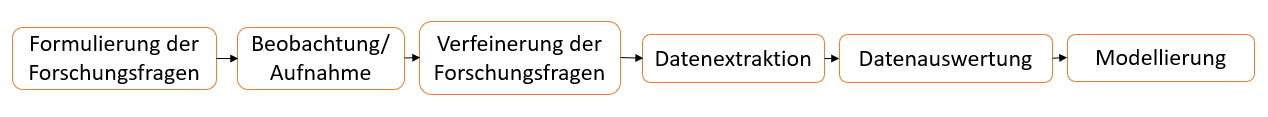
\includegraphics[width=1.0\textwidth]{pictures/introduction/strukture/strukture_work.png}
	\caption{Struktur des Vorgehens in bei der Modellfindung für diese Bachelorarbeit}
	\label{fig:Vorgehen}
\end{figure}
 
\section{Begriffe und Definitionen} \label{Begriffe und Definitionen}
Im Folgenden werden Begriffe definiert, die ich verwende, um den Fahrgastwechsel zu beschreiben. 
\begin{longtable}{ l p {10 cm}}
			 \textbf{Aussteiger}	& Personen die vom Inneren des Zuges auf den Bahnsteig gelangen wollen.\\
			 	& \\
			 \textbf{Einsteiger}	& Personen die vom Bahnsteig in das Innere des Zuges gelangen wollen.\\
				& \\
			 \textbf{Platzmacher}	& Personen, die aus dem Zug aussteigen, um anderen Personen im Zug die Möglichkeit zu geben, auszusteigen. Diese Personen wollen danach wieder in den Zug gelangen.\\
				& \\
			\textbf{Türbereich}	& Bereich zwischen den Türen des Zuges, der beim Ein- und Aussteigen betreten werden muss. Siehe \figurename \ref{fig:Doorarea}\\
				& \\
			\textbf{Fahrgastwechselzeit}	& Die Zeit, die es dauert, bis der Fahrgastwechsel beendet ist. Der Fahrgastwechsel beginnt, wenn der erste Aussteiger den ersten Fuß auf den Bahnsteig setzt. Ist kein Aussteiger vorhanden oder existiert eine Person die einsteigt, bevor der erste Aussteiger mit dem Aussteigen beginnt,  so beginnt der Fahrgastwechsel, wenn der erste Einsteiger einen Fuß in den Wagon setzt. Der Fahrgastwechsel ist beendet, wenn der letzte Einsteiger seinen zweiten Fuß in den Wagon setzt. Falls keine Einsteiger vorhanden ist, oder noch ein Aussteiger aus dem Zug tritt, wenn schon alle Einsteiger im Wagon sind, wird der Fahrgastwechsel beendet, wenn der letzte Aussteiger seinen zweiten Fuß auf den Bahnsteig setzt.\\
				& \\
			\textbf{Prozesstypen}	& Einsteiger, Aussteiger und Platzmacher bilden die verschieden Prozesstypen.\\
				& \\
			\textbf{Personen}	& Wird in dieser Bachelorarbeit in Bezug auf den Fahrgastwechsel das Wort "`Personen"' verwendet ist damit immer die Gesamtheit der Personen gemeint, die an dem Fahrgastwechsel beteiligt sind. Also die Summe aller Einsteiger, Aussteiger und Platzmacher dieses Wechsels.
\end{longtable}

 \begin{figure}[H]
	\centering
		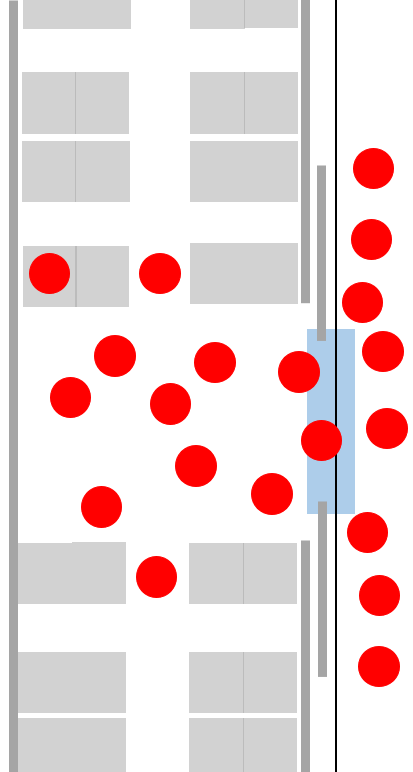
\includegraphics[angle=270, width=0.5\textwidth]{pictures/introduction/defenitions/example_doorarea.png}
	\caption{Skizze zur Erklärung des Begriffes "`Türbereichs"' aus der Vogelperspektive: U-Bahn "`Wände"' dargestellt durch graue Linien, Sitzplätze der U-Bahn durch graue Vierecke, Bahnsteigkante durch schwarze Linie, Fahrgäste durch rote Kreise. Der Türbereich ist durch ein blaues Rechteck gekennzeichnet.}
	\label{fig:Doorarea}
\end{figure} 
\todo{Überprüfen alle Begriffe definiert}
\section{Formatierung}
\begin{table}[H]
	\centering
		\begin{tabular}{ l p {12 cm}}
		\textsf{Sans Sherif}	& Die Schriftart "`Sans Sherif"' wird verwendet, um Software zu beschreiben. Sie wird eingesetzt, wenn der Name einer Software verwendet wird.\\
		\texttt{Typewriter}	& Die Schriftart "`Typewriter"' wird für Namen bei der Auswertung verwendeter Python Bibliotheken und Funktionen benutzt. \\
		\textsl{Slanted}	& Die Schriftart "`Slanted"' wird bei Verweisen auf Zusatzmaterial verwendet, Dateiname wird dabei mit dieser Schriftart geschrieben.
		\end{tabular}
\end{table}
\chapter{Beobachtung} \label{Beobachtung}
Um ein realistisches Modell erstellen zu können, führte ich empirische Beobachtungen an drei großen Haltestellen der Münchener U-Bahn durch. Für die spätere Auswertung habe ich hierbei Aufnahmen des Fahrgastwechsels angefertigt. Das dabei entstandene Bildmaterial, kann auf dem der Arbeit beigelegten Stick betrachtet werden. Die Anfertigung der Aufnahmen beschreibe ich im Folgenden. 
\section{Aufnahmen der Beobachtung} \label{Aufnahmedetails}
Zum Aufnehmen des Wechselprozesses nahm ich einen Platz auf den an U-Bahn-Stationen vorhandenen Wartebänken ein. Von diesem Platz aus konnte ich bei Einfahren des Zuges immer eine Tür frontal aufnehmen. Eine beispielhafte Skizze, für die Position, aus der ich beobachtete, kann in \figurename \ref{fig:skizzeBeobachtung} betrachtet werden. \\
\begin{figure}[H]
	\centering
		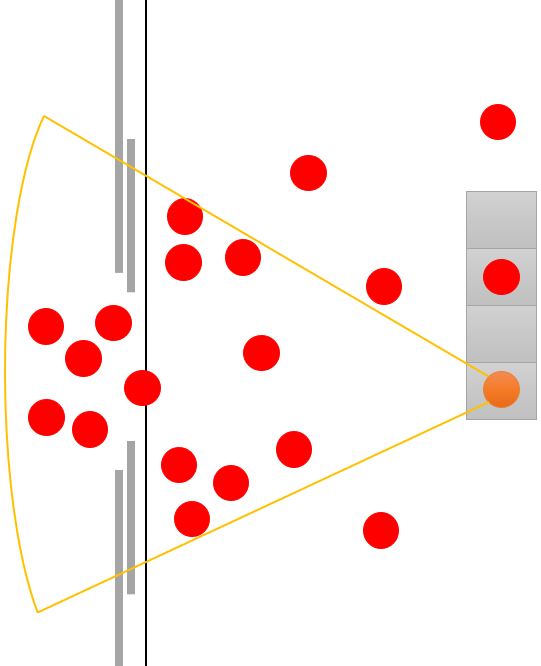
\includegraphics[angle=270, width=0.6\textwidth]{pictures/observation/recording/example_tapping.png}
	\caption{Skizze der Aufnahme an Bahnsteigen aus der Vogelperspektive. Die grauen Rechtecke stellen die Bänke des Bahnhofes dar. Hellgraue Linien zeigen die "`Wände"' des Zuges. Die schwarze Linie zeigt die Bahnsteigkante. Die roten Kreise repräsentieren Fahrgäste, während der orange Punkt die filmende Person darstellt. In Gelb ist der Bereich eingezeichnet, der von der Kamera eingefangen wurde.}
	\label{fig:skizzeBeobachtung}
\end{figure}
Zum Filmen der Türen verwendete ich die Kamera "'Canon EOS 650D"'. Für jeden einfahrenden Zug erstellte ich ein Video. Die Aufnahmen der U-Bahnen fanden zwischen dem 26. März und 25. Mai 2019 statt. Die Aufnahmen fertigte ich dabei zwischen 8:00 und 18:00 Uhr an. Im angegebenen Zeitraum wurden 67 Videos aufgenommen von denen 56 Videos für die Weiterverarbeitung geeignet waren. Auf den anderen Videos stehen Personen derart im Weg, dass eine Auswertung des Fahrgastwechsels nur sehr ungenau oder gar nicht möglich gewesen ist. Somit beobachtete ich 56 Türen, an denen ein Fahrgastwechsel stattfand. Dabei nahm ich 1173 Personen auf Video auf. Die Beobachtungen fanden an 3 großen Haltestellen der MVG statt: am Marienplatz München, am Odeonsplatz und am Hauptbahnhof. Während der Beobachtung nahm ich mit einer Kamera auf, wie der Fahrgastwechsel abläuft. Die gefilmten Fahrgäste wurden nicht darüber informiert, dass ich sie beobachtete und aufnahm, um ihr Verhalten nicht zu beeinflussen. Das ist zulässig, weil die Aufnahmen nicht veröffentlicht werden, sondern nur der Datenerhebung dienen. Videos oder Bilder, die der Veranschaulichung dienen, anonymisiere ich vor der Veröffentlichung komplett: auf dem Bildmaterial aufgenommene Personen werden unkenntlich gemacht. In dieser Arbeit verwendete ich zwei Methoden zur Verfälschung der Identitäten. Zum einem bearbeitete ich Bilder mit dem Bildbearbeitungsprogramm \textsf{GIMP}. Bei der Bearbeitung verpixele ich die Gesichter der Personen so, dass diese nicht mehr erkennbar sind. Zudem verwendete ich zur Bearbeitung von Bildern und Videos den Code eines Kommilitonen, Andre Heinrich. Dieser erstellte in einem vergangenen Semester einen Filter in \textsf{Jupyter Notebook} der ein Bild comicartig zu Strichzeichnungen vereinfacht.
Die \figurename \ref{fig:PersonenUberZeit} zeigt genauer, zu welchen Zeiten Videos aufgenommen wurden, und wie viele Personen zu diesen Zeiten durchschnittlich am Fahrgastwechsel beteiligt waren.
\begin{figure}[H]
	\centering
		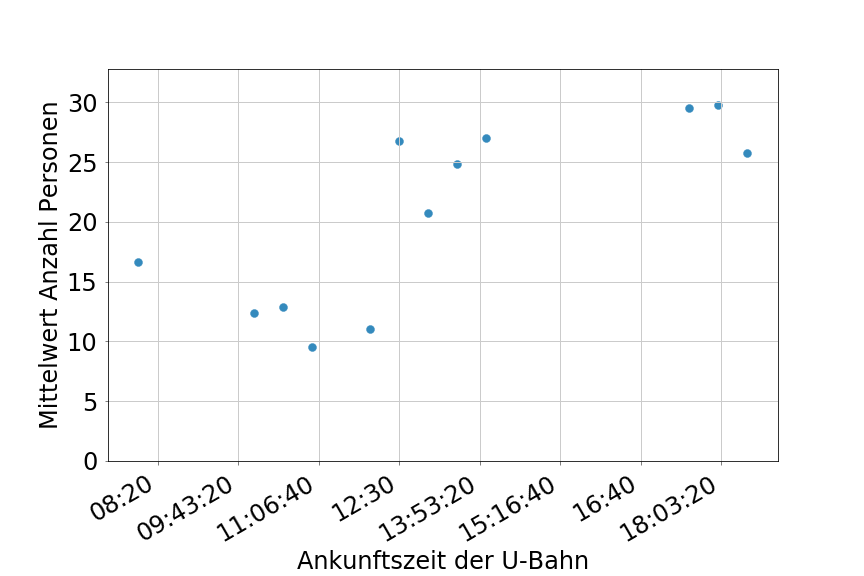
\includegraphics[width=1.0\textwidth]{pictures/observation/recording/peopleOverTime.png}
	\caption{Mittelwert der Anzahl der Beobachteten zu aufgenommenen Zeiten.}
	\label{fig:PersonenUberZeit}
\end{figure}
In diesem Plot kann erkannt werden, dass die höchsten Werte für die Anzahl an Personen zwischen 17:00 und 18:00 Uhr erreicht wurden. Dieses Ergebnis stimmt mit den Angaben der Deutschen Bahn überein, welche angibt, dass ihre Hauptverkehrszeiten zwischen 6:30 und 9:30 Uhr sowie 15:30 und 18:30 liegen (\cite{DeutscheBahnAG.2018}). Die hohen Werte zwischen 12:30 und 15:00 wurden am Wochenende aufgenommen. Die Angaben der Deutschen Bahn beziehen sich auf Hauptverkehrszeiten unter der Woche.
\section{Standardfall}
Im Standardfall der Beobachtungen ist ein einigermaßen ausgeglichenes Verhältnis an ein- und aussteigenden Personen gegeben. Wollen Personen in den einfahrenden Zug einsteigen, begeben sie sich in an die Türen der U-Bahn. Wollen auf dem Bahnsteig wartende Fahrgäste jedoch nicht in diesen Zug einsteigen, so verbleiben diese auf ihrer Position in gewissem Abstand von den Gleisen. Begeben sich die Einsteigenden an den Zug, positionieren diese sich im Normalfall rechts und links der Tür, um den Aussteigenden Platz zu gewähren. Dieser Fall kann in \figurename \ref{fig:normalerFahrgastwechsel} beobachtet werden.
\begin{figure}[H] 
	\centering
		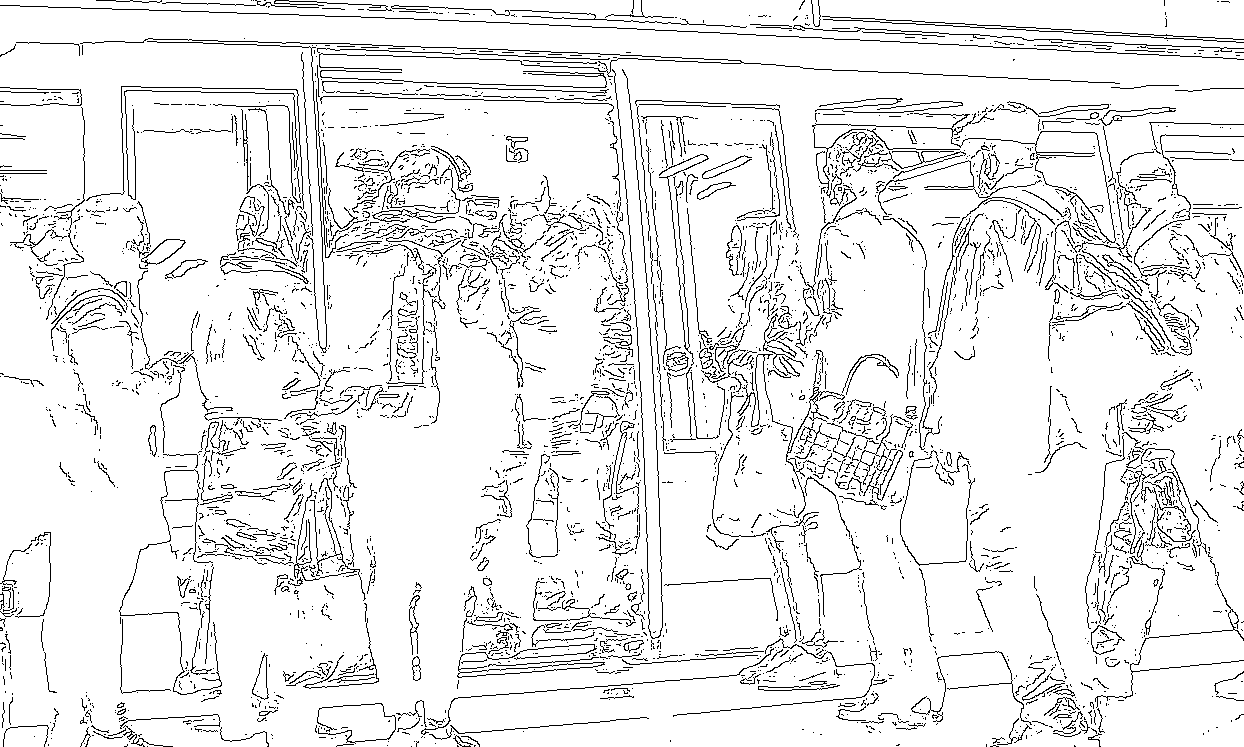
\includegraphics[width=0.8\textwidth]{pictures/observation/standard/exchange.png} 
	\caption{Fahrgastwechsel mit Einsteigern und Aussteigern im Standardfall.}
	\label{fig:normalerFahrgastwechsel}
\end{figure} 
Aussteigende beginnen sich aus dem Zug zu bewegen, wenn die Türen geöffnet werden und steigen normalerweise in Zweierreihen aus dem Zug aus. Im häufigsten Fall beginnen die Einsteiger dann mit dem Einsteigeprozess, wenn alle Aussteigenden aus der Tür ausgestiegen sind.
\section{Sonderfall: Beobachtungen vor einem Fußballspiel} \label{Fussballspiel}
Im Beobachtungszeitraum fand in München ein großes Fußballspiel statt. Einer der Münchner Fußballvereine, der FC Bayern München, spielte am 6. April 2019 gegen den Dortmunder Verein BVB (Ballspiel-Verein-Borussia). Da es mich interessierte, ob sich das Verhalten der Ein- und Aussteiger bei einer solchen Veranstaltung verändert, habe ich an diesem Tag den Fahrgastwechsel beobachtet. Die Beobachtungen fanden vor Beginn des Fußballspiels statt. Die observierten Personen befanden sich somit auf dem Weg zum Stadion. Einflüsse auf das Verhalten durch das Ergebnis des Spieles konnten somit nicht in die Daten eingehen. Die Unterschiede zu Beobachtungen an Tagen ohne Veranstaltungen werden im Folgenden kurz erläutert und mögliche Erklärungen für diese Unterschiede beschrieben. 
\subsection{Unterschiede}
Zunächst ist zu erwähnen, dass sich das Verhältnis von Einsteigern zu Aussteigern deutlich veränderte. An der beobachteten Station, dem Marienplatz München, stiegen in diesem Zeitraum, trotz vieler Personen im Zug, nur sehr wenige Personen aus.\\ 
Abgesehen vom Unterschied im Verhältnis der Prozesstypen konnte auch eine Veränderung im Verhalten beobachtet werden. Vor dem Fußballspiel positionierte sich ein Großteil der Personen nah am Bahnsteig. Somit standen diese Wartenden auch direkt am Zug, und damit auch an den Türen, wenn sie nicht in den Zug einsteigen wollten.\\
Ein weiterer Unterschied ließ sich darin erkennen, wie Fahrgäste sich an die Türen stellten. In dem beobachteten Zeitraum vor dem Fußballspiel konnte diese Verhaltensweise des rechts und links Stehens vor der Tür nicht erkannt werden. Bei dieser Beobachtung standen alle wartenden Personen direkt am Eingang des Wagons, wie in \figurename \ref{fig:fussballFahrgastwechsel} zu sehen ist. Aussteiger mussten sich einen Weg durch die Masse suchen und konnten nicht auf geradem Weg den Zug verlassen. Auch die zuvor beschriebenen Personen, welche nicht in den Zug gelangen wollten, versperrten einen Großteil des Weges für Aussteigende. \\
\begin{figure}[H]
	\centering
		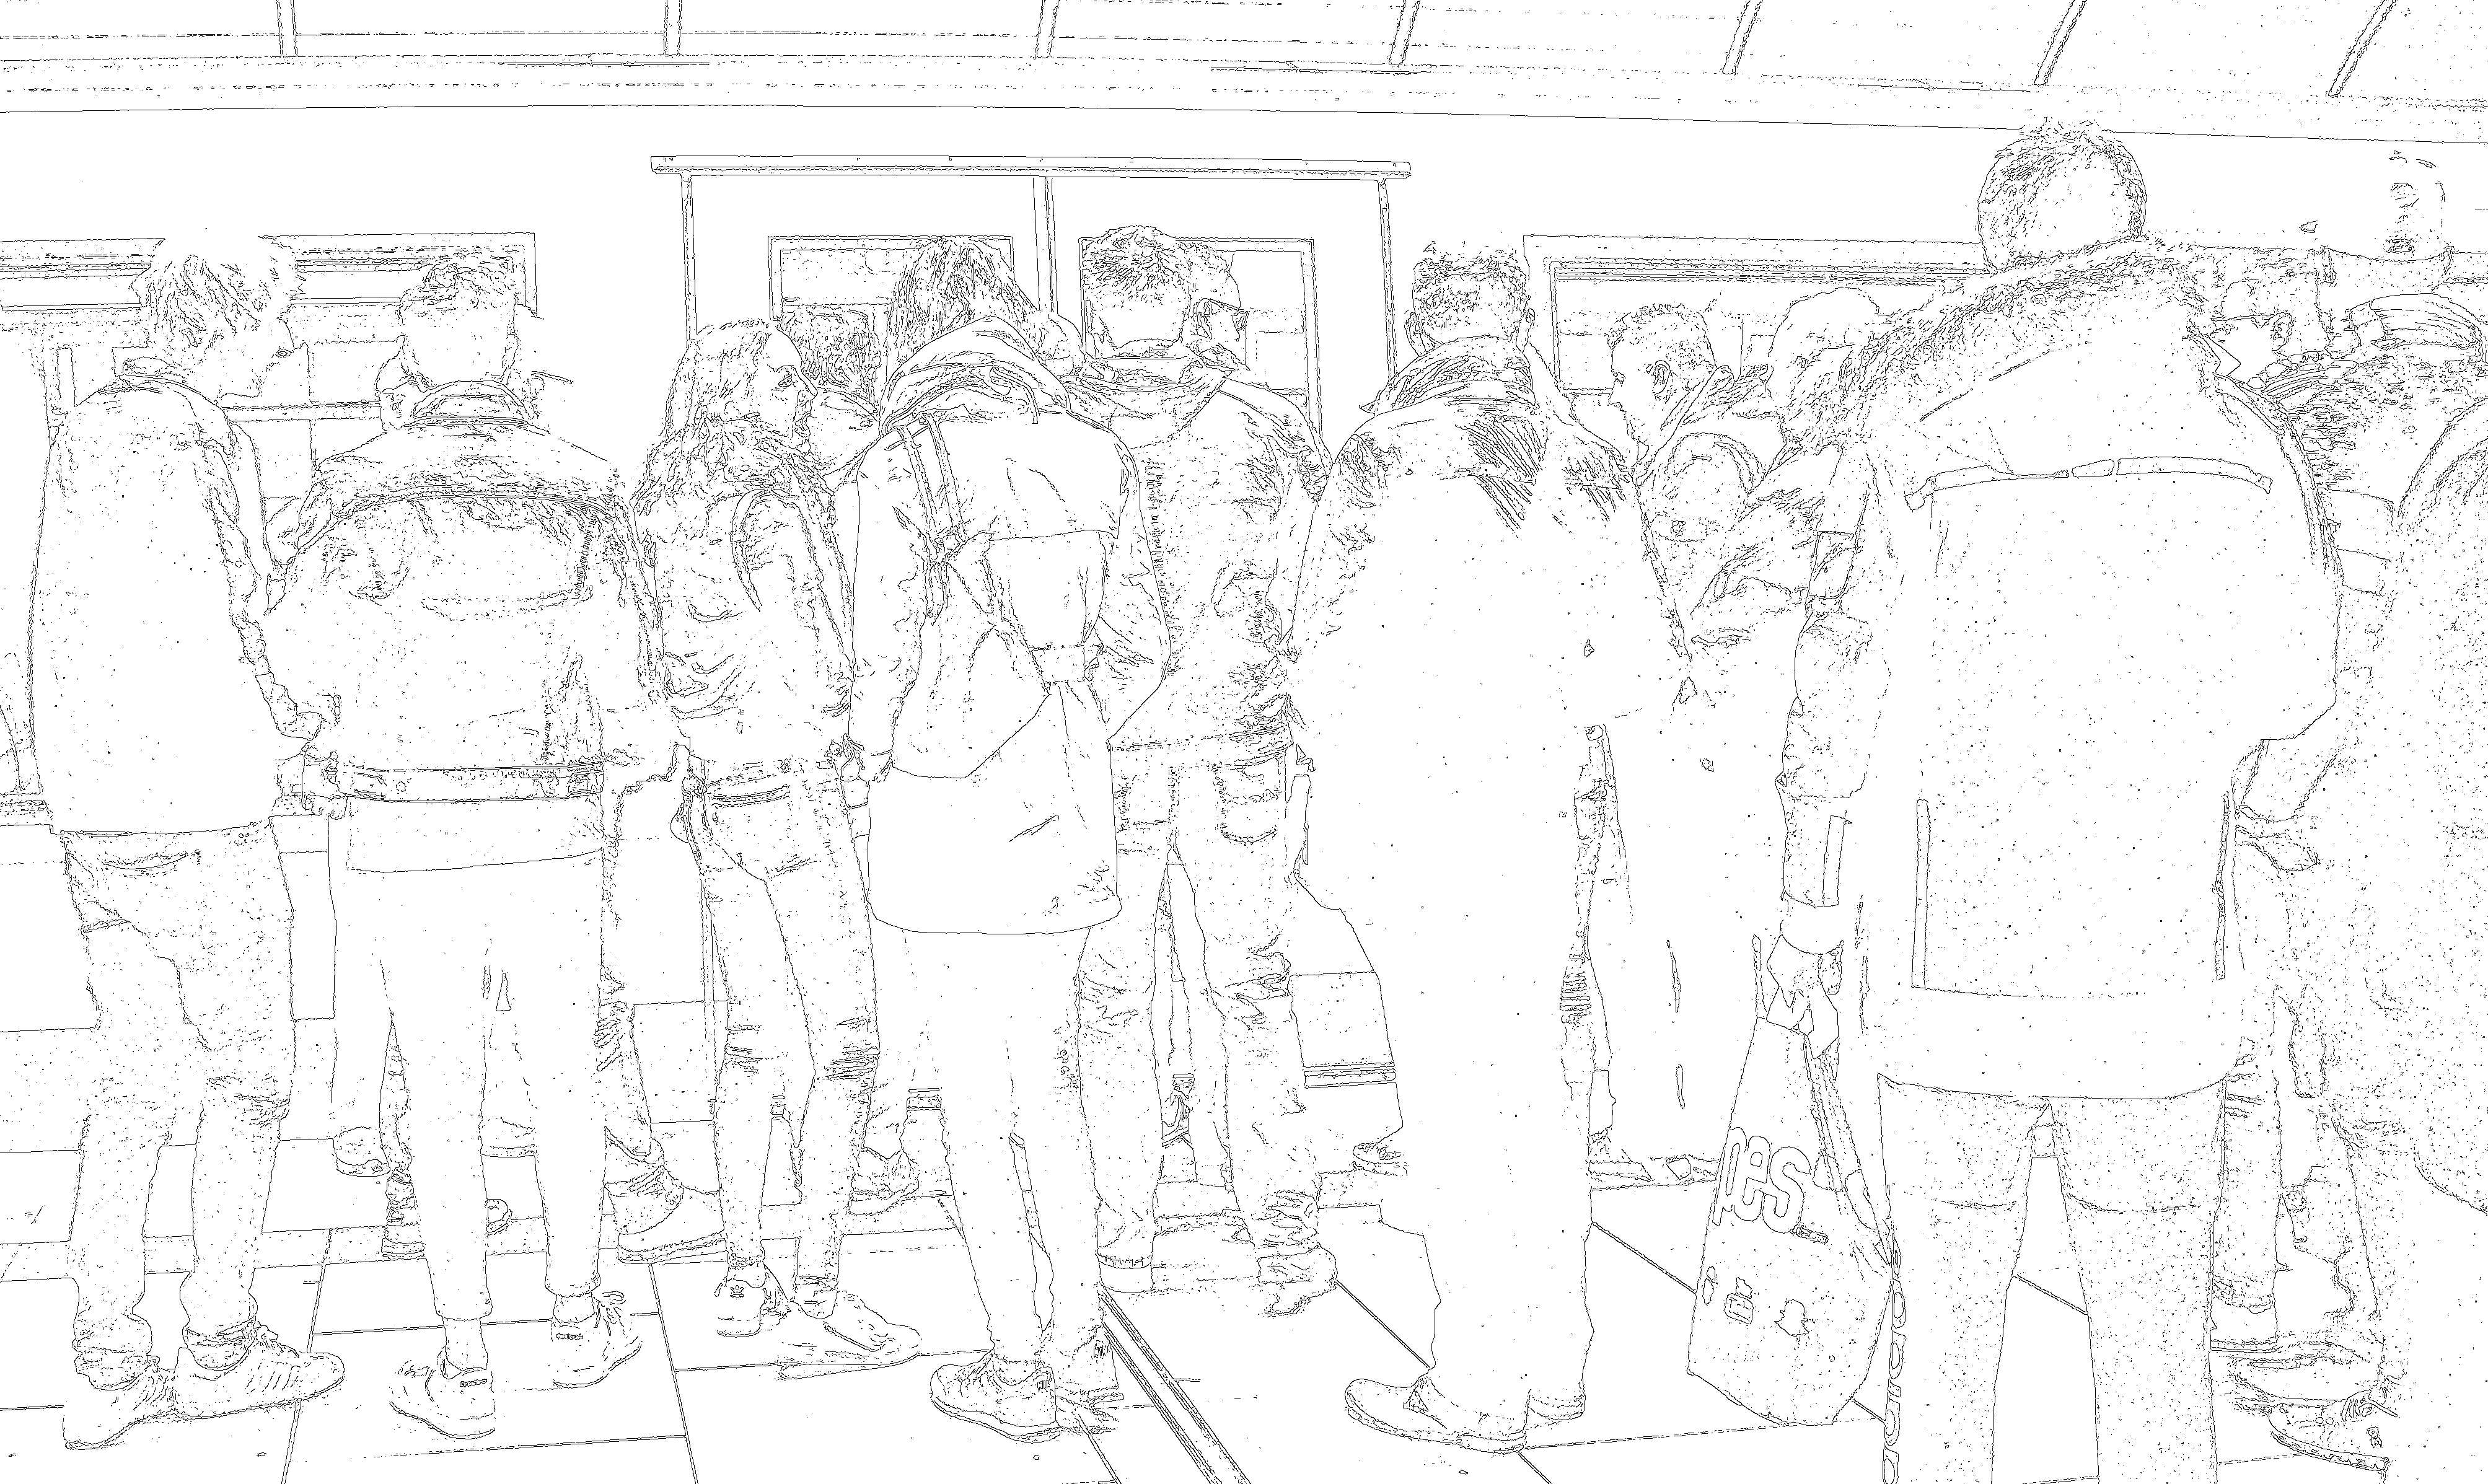
\includegraphics[width=0.8\textwidth]{pictures/observation/football/exchange_football.png}
	\caption{Fahrgastwechsel vor dem Fußballspiel, FC Bayern gegen BVB, mit wartenden Personen.}
	\label{fig:fussballFahrgastwechsel}
\end{figure}
\subsection{Einflussfaktoren}
Nachdem die Unterschiede festgestellt wurden, soll nun erklärt werden, welche Einflussfaktoren diese Veränderung hervorgerufen haben könnten.
Ein Einflussfaktor für das beobachtete Verhalten könnte die andere Verteilung an Ein- und Aussteigern sein. Da nur sehr wenige Personen aus dem Zug gelangen wollen, könnte die Hemmschwelle, diesen im Weg zu stehen, sinken. Dies kann jedoch nicht der einzige Grund für das veränderte Verhalten sein. Bei Zügen, die außerhalb des Fußballspieles beobachtet wurden und bei denen nur wenige Personen ausstiegen, wurde dieses Verhalten nicht beobachtet. Deshalb ist davon auszugehen, dass das Verhältnis nicht der einzige Grund für das im Weg stehen ist.\\
Um die Unterschiede erklären zu können, müssen also die beteiligten Personen genauer betrachtet werden. Einer der Unterschiede bei den Fahrgästen liegt im Alkoholkonsum. Im normalen Beobachtungszeitraum führte keiner der Fahrgäste Alkohol mit sich und keiner der Beobachteten wirkte alkoholisiert. Bei den Beobachtungen vor Beginn des Fußballspiels machten jedoch einige der Fahrgäste einen alkoholisierten Eindruck oder trugen alkoholische Getränke bei sich. Neben dem Alkoholkonsum fiel auf, dass sich auch die Stimmung bei diesen Beobachteten von der im Standardfall unterschied. Die meiste Zeit war die Stimmung gelöst, es wurde gesungen und U-Bahn-Wagons durch Auf- und Abspringen zum Schwanken gebracht. Diese andere Stimmung könnte ein weiterer Einflussfaktor dafür sein, dass sich das Verhalten der Passagiere verändert. \\
Die Beobachtungen zum Fußballspiel liefern interessante Ergebnisse. Da dies jedoch, in den Beobachtungen dieser Arbeit, ein absoluter Sonderfall ist, fließen sie nicht in das Modell mit ein. Eine genauere Untersuchung könnte jedoch zu einem Modell für einen solchen Spezialfall führen, welcher wiederum für eine Verbesserung der Planung der Abläufe im öffentlichen Nahverkehr führen könnte.
\chapter{Forschungsfragen} \label{Forschungsfragen}
Um eine Entscheidung darüber zu treffen, welche Daten des Fahrgastwechsels aus den Videos erhoben werden sollen, verfeinere ich Forschungsfragen aus Abschnitt \ref{Stand der Technik}. Im Folgenden wiederhole diese Fragen und nenne jeweiligen Verfeinerungen, falls vorhanden.
\begin{enumerate}
 \item "`Kann die Fahrgastwechselzeit aus der Anzahl der Aus-, Einsteiger und Platzmacher abgeschätzt werden?"' (Auswertung in Abschnitt \ref{Zeiten}) \label{item:Fahrgastwechselzeiten}
 \item "`Welche Verhaltensweisen und Merkmale von Fahrgästen beeinflussen die benötigte Zeit für den Fahrgastwechsel?"' \label{item:Verhalten}
 	\begin{enumerate}
 		\item "`Beeinflussen die Verhaltensweisen "`früher Einsteigen"' und "`Im Weg Stehen"' die Fahrgastwechselzeiten?"' (Beschreibung der Verhaltensweisen in \ref{Datenerhebung}, Auswertung in \ref{Verhalten}) \label{item:Verhalten,Verhalten}
 		\item "`Beeinflussen die Merkmale "`sperrig"', "`langsam"' und "`abgelenkt"' der Fahrgäste die Fahrgastwechselzeit?"' (Beschreibung der Merkmale in \ref{Datenerhebung}, Auswertung in \ref{Verhalten}) \label{item:Vehalten,Merkmale}
 	\end{enumerate}
 \item "`Welche Entscheidungen werden beim Prozess des Fahrgastwechsel getroffen?"' (Auswertung in Kapitel \ref{Modell}) \label{item:Entscheidungen}
\end{enumerate}
Zudem kamen noch folgende Forschungsfragen auf:
\begin{enumerate}
\setcounter{enumi}{3}
	\item "`Gibt einen Zusammenhang zwischen der Anzahl der Aussteiger und dem Vorkommen von Platzmachern?"' (Auswertung in \ref{Verhalten})  \label{item:Platzmacher}
	\item "`Kann aus dem Filmmaterial gewonnen werden, welche Gruppengrößen im Fahrgastwechsel auftreten und wie viel Prozent der Personen sich in einer Gruppe mit einer bestimmten Größe befinden?"' Die Größe einer Gruppe wird definiert durch die Anzahl ihrer Mitglieder. Mitglied einer Gruppe ist, wer zu mindestens einem anderen Mitglied der Gruppe Kontakt hat, \dahe er mit einem Mitglied der Gruppe redet oder auf ein Mitglied der Gruppe wartet. \label{item:Goupsize} 
	\item Auf den Videos wurden Verhaltensweisen, erkannt die als "`defensiv"' oder "`aggressiv"' bezeichnet werden können. Dazu gehören unter anderem Verhaltensweisen wie das in den Weg anderer Personen laufen oder mit dem Einsteigen warten bis alle aus dem Zug sind, auch wenn genug Platz zum Einsteigen wäre. Zeigte eine Person eine oder mehrere dieser Verhaltensweisen wurde sie als "`defensiv"' oder "`aggressiv"' bezeichnet. Zeigte sie keine dieser Verhaltensweisen galt die Person als "`normal"'. Wie die Personen in diese Typen (aggressiv, defensiv und normal) eingeteilt wurden wird in \ref{Tabelle der Typen} genauer erklärt. Um herauszufinden ob die Einteilung in Typen für das Modell interessant ist soll die Frage: "`Gibt es einen signifikanten Anteil an defensiven und aggressiven Personen?"' geklärt werden.(Auswertung in Abschnitt \ref{Typen}) \label{item:Typen,Typen}
	\begin{enumerate}
		\item Nachdem mir auffiel, dass die unterschiedlichen Typen von Aussteigern unterschiedlich lange warten, bis sie aussteigen, kam zudem die Frage auf: "`Liegen die Startzeiten der Aussteiger für die unterschiedlichen Typen in unterschiedlichen Intervallen?"' (Auswertung in Abschnitt \ref{Startzeiten}) \label{item:Typen,Startzeiten}
	\end{enumerate} 
\end{enumerate}
\chapter{Datenextraktion} \label{Datenerhebung}
Nachdem ich die Forschungsfragen verfeinert habe, erhebe ich Merkmale und Zahlen aus den Videos, die der Beantwortung dieser dienen. Ich betrachte die Videos qualitativ und fertige Tabellen an, die Anzahlen der Personen mit gewissen Merkmalen und Verhaltensweisen, sowie Wechselzeiten enthalten. In diesem Kapitel erkläre ich die Methoden der Datenerhebung aus den Videos. Zudem gehe ich darauf ein, wie ich die Merkmale und Verhaltensweisen der Personen definiere.
\section{Methode der Extraktion: Tracking}\label{Tracking}
Bei der ersten Sichtung des Bildmaterials fiel mir ein Problem bei den Aufnahmen auf. Das frontale Filmen der Türen führt dazu, dass Fahrgäste, die nicht am Fahrgastwechsel der gefilmten Tür beteiligt sind, die Sicht auf diese versperren. Beispielhaft für dieses Problem ist die Abbildung \ref{fig:Problem bei Videos}.
\begin{figure}[H]
	\centering
		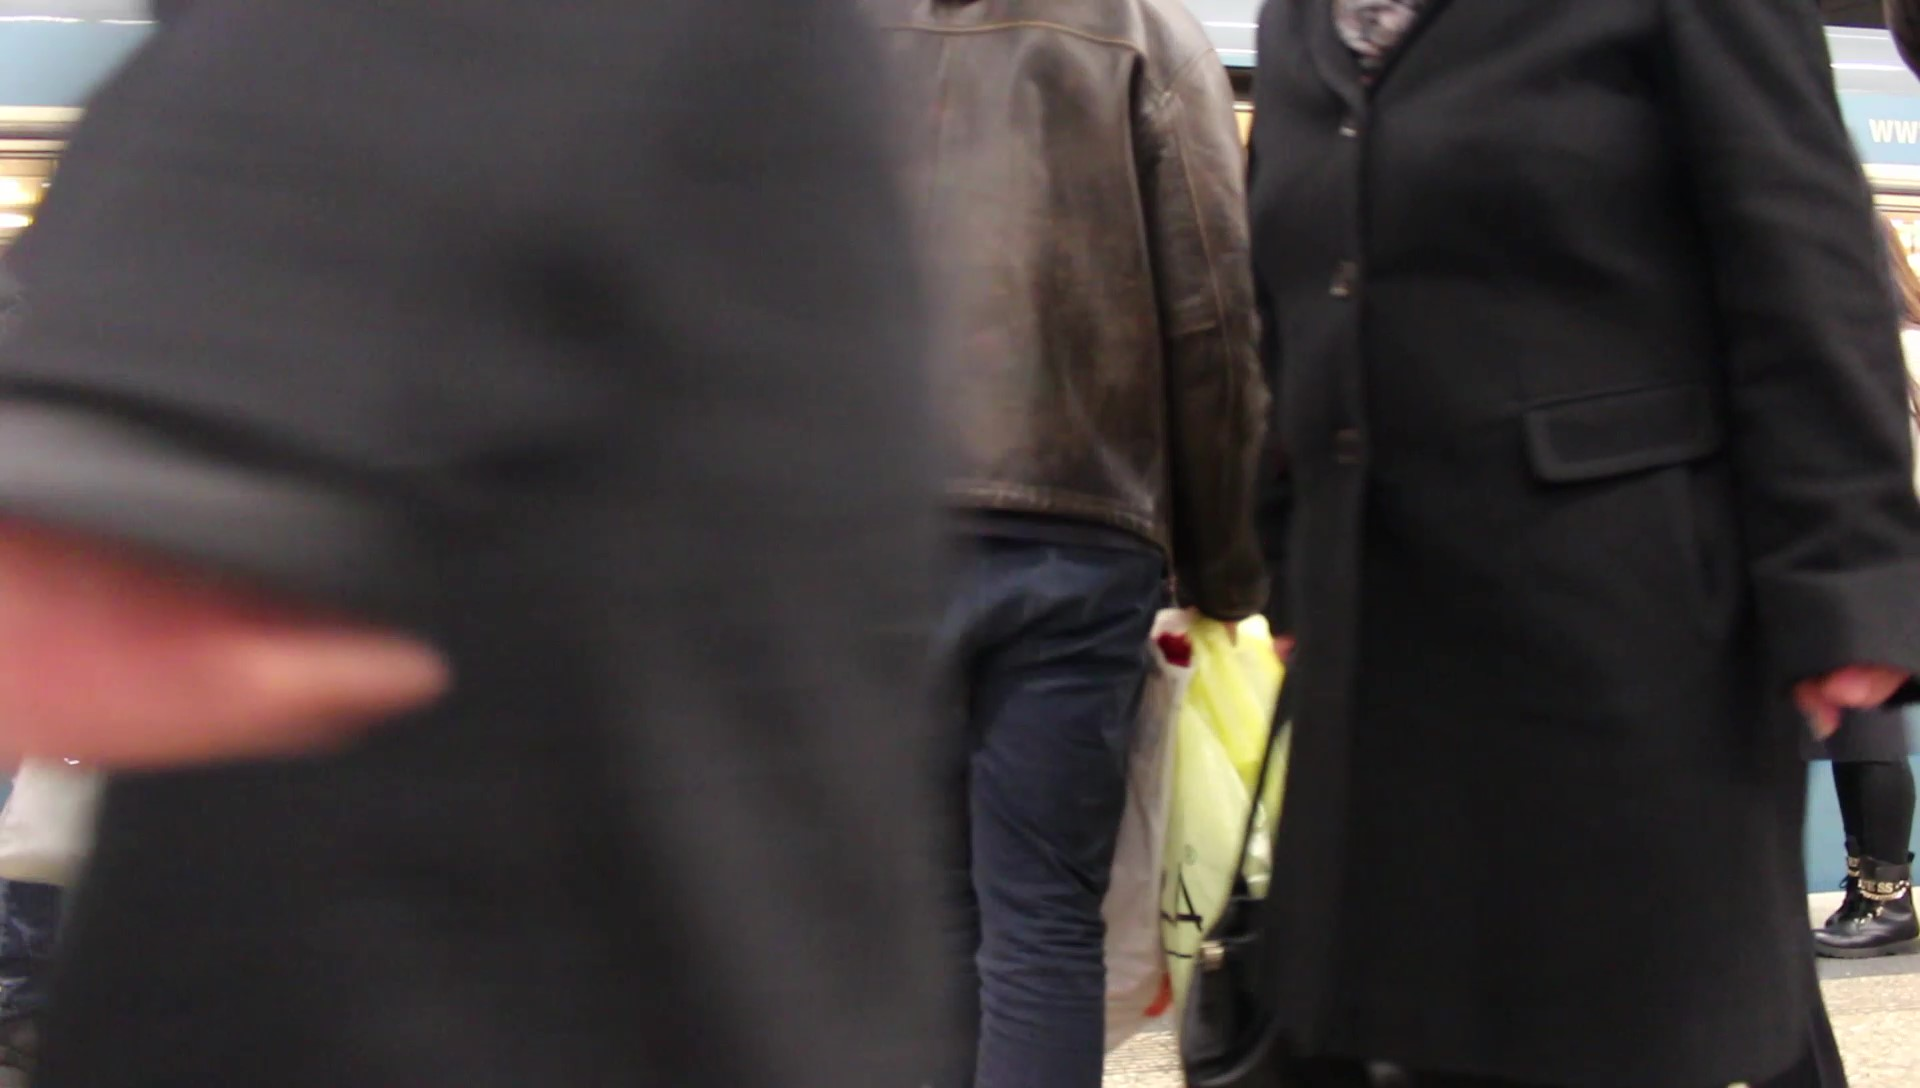
\includegraphics[width=0.65\textwidth]{pictures/data_extraction/tracking/problem.jpg}
	\caption{Beispiel für Probleme mit der Aufnahme: Personen, die durch das Bild laufen, versperren die Sicht auf den Fahrgastwechsel in der Tür. Quelle: Eigene Darstellung.}
	\label{fig:Problem bei Videos}
\end{figure} 
Auf diesem Bild ist zu erkennen, dass die Sicht auf den Fahrgastwechsel in der gefilmten Tür versperrt ist.\\
Um eine genaue Zählung trotz dieses Problems zu ermöglichen, benutze ich die mir aus einem früheren Semester bekannte Software \textsf{Tracker}. Die Tracking-Dateien können auf dem beigelegten Stick gefunden werden. Mit dieser Software kann ich die Videos Einzelbild für Einzelbild (eng.: "`Frame"') betrachten. Dadurch kann ich die Personen genauer zählen. Die Ansicht jedes Bildes ermöglicht mir zudem ein genaueres Messen der Fahrgastwechselzeiten. Die Einzelbilder, in denen der Fahrgastwechsel beginnt und endet kann ich so eindeutig identifizieren, wenn die Sicht auf die Tür frei ist. Die zugehörige Sekunde des Einzelbildes wird in der Software auf 3 Stellen genau angezeigt. Mit diesen genauen Zahlen kann ich dann genauer die Zeit messen, welche die Personen für den Wechsel benötigt haben. Jedoch nahm ich auch Filme auf, bei denen eine Person durch das Bild ging, wenn gerade die letzte Person einstieg. Dadurch kann ich auf diesen Videos das genaue Einzelbild des Fahrgastwechselendes nicht identifizieren. Für Filme, in denen dies geschah, schätzte ich den Moment, in dem das zweite Bein in den Wagen gesetzt wird. Im schlimmsten Falle wurde die Sicht auf den letzten Einsteiger 21 Frames lang versperrt. Ich schätzte jedoch, dass der Moment, in dem der zweite Fuß in den Wagon gesetzt wurde innerhalb von 10 der 21 Frames geschehen musste. Bevor die Person in das Bild gelaufen ist, war der Einsteiger noch etwas von der Tür entfernt und als die Person wieder aus dem Bild gegangen war, war die Person schon ein paar Schritte in den Zug gegangen. Deshalb konnten 6 Frames, nachdem die Person ins Bild gelaufen ist und 5 Frames bevor die Person wieder aus dem Bild ging, mit Sicherheit als nicht mögliche Zeitpunkte für das Fahrgastwechselende eliminiert werden. Ich schätze den Messfehler also auf \ca 10 Frames und damit, da ein Frame 0.033 Sekunden darstellt, auf 0.33 Sekunden. Deshalb wird ab nun die Fahrgastwechselzeit auf eine Stelle nach dem Komma gerundet.\\
Neben der Einzelbildansicht gibt es in diesem Tool die Möglichkeit, jeder Person eine sogenannte Punktmasse zuzuordnen und diese zu tracken. Dadurch wird verhindert, dass ein Fahrgast doppelt gezählt wird. Zudem kann ich dadurch das Verhalten und die Merkmale einer einzelnen Person über den gesamten Prozess besser beobachten. Der \textsf{Tracker} bietet zwei Möglichkeiten des Trackens. Zum einen kann eine Masse per Auto-Track verfolgt werden, zum anderen können die Personen per Hand in jedem Bild getrackt werden. Durch das Problem der versperrten Sicht war es nicht möglich das Auto-Tracking zu verwenden. Jede Person wurde von mir per Hand getrackt. In \figurename \ref{fig:tracking} kann das Tracking auf einem Bild eines der Videos betrachtet werden. Um den Vorgang des manuellen Trackings zu vereinfachen, tracke ich Aussteigende in unterschiedlichen Rottönen, Einsteigende in unterschiedlichen Blautönen. Platzmacher - auf diesem Bild nicht vorhanden - markierte ich in Grüntönen. \\
\begin{figure}[H]
	\centering
		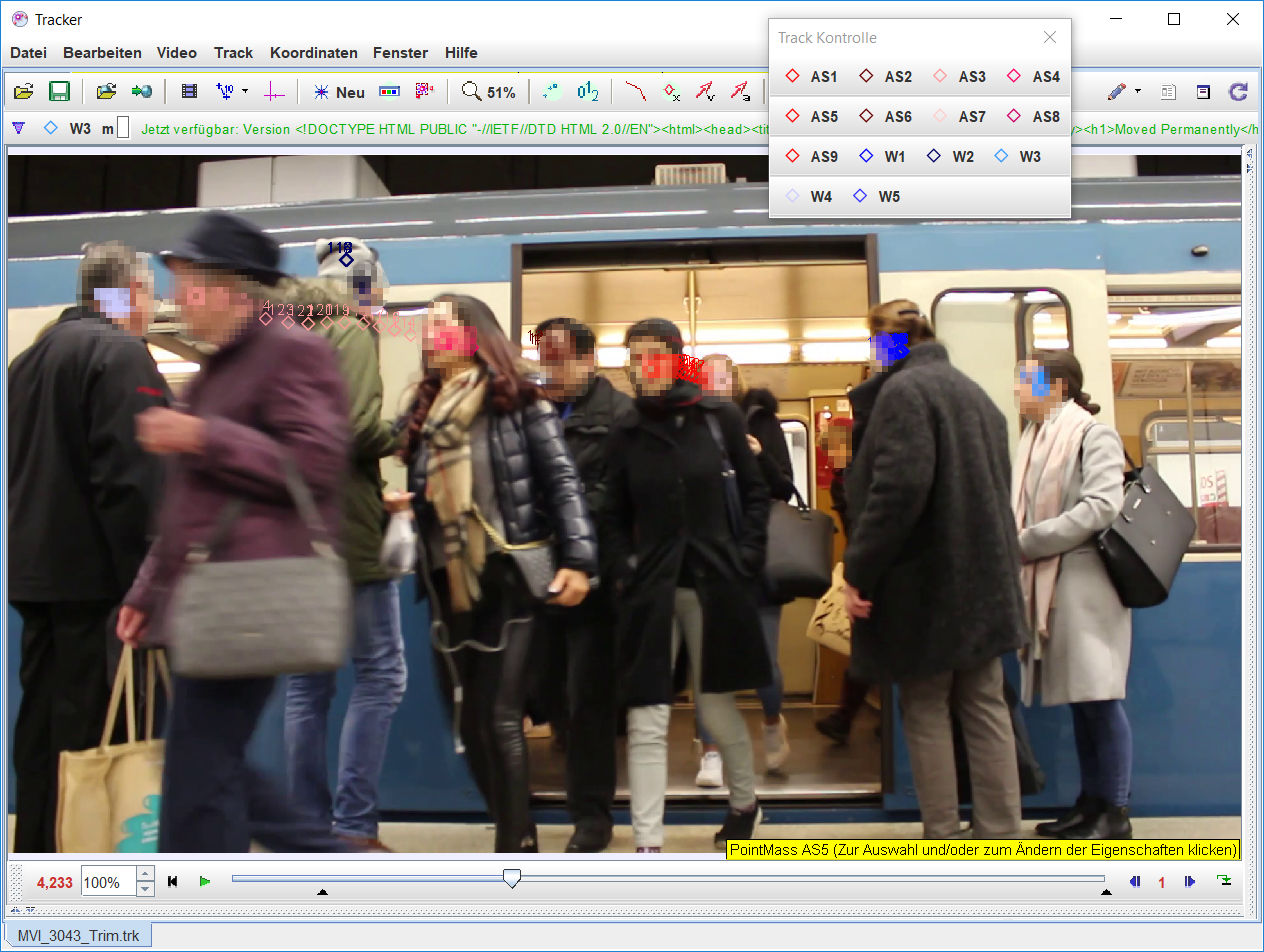
\includegraphics[width=0.7\textwidth]{pictures/data_extraction/tracking/trackExample.png}
	\caption{Screenshot der Software \textsf{Tracker}, mit Video und getrackten Personen. Aussteiger sind mit Rot, Einsteiger mit Blau gekennzeichnet. Quelle: Eigene Darstellung.}
	\label{fig:tracking}
\end{figure}
\section{Tabellen} \label{Tabellen}
Für die unterschiedlichen Forschungsfragen erstellte ich Excel-Dateien, welche die Anzahlen von Personen und Zeiten enthalten, die ich mit dem Tracking-Tool aus den Videos gewonnen habe. Bei der Datenerhebung erstellte ich sieben CSV-Dateien in Excel. Die Tabellen sind auf auf GitHub frei zugänglich: \url{https://github.com/AlexandraMayer/Bachelorarbeit-Fahrgastwechsel---Alexandra-Mayer-26.08.2019/tree/master/Tabellen_Notebooks/Tabels}. Dabei enthalten die einzelnen Dateien jeweils  Verhaltensweisen, Merkmale, Typen von Personen, Startzeiten der Aussteiger, Fahrgastwechselzeiten, sowie die erkannten Gruppen. Die Kopfzeilen der Tabellen sind in Englisch verfasst, um Probleme mit Umlauten bei der Weiterverarbeitung zu verhindern. \\
Jede Zeile der Tabellen enthält die jeweilige Anzahl der Merkmale und Verhaltensweisen und Zeiten für ein einzelnes Video. Diese trug ich nach der Sichtung des jeweiligen Videos in die entsprechenden Spalten ein. Zudem enthält die erste Spalte der Tabellen immer die Zahl des jeweiligen Videos (wie im Videonamen angegeben) um eine Zuordnung zu dem entsprechenden Film zu gewährleisten.
\subsection{Tabelle der Fahrgastwechselzeiten} \label{Zeiten Tabelle}
In der Tabelle der Fahrgastwechselzeiten hielt ich die Anzahlen der Kern-Einsteiger und Später-Einsteiger, sowie der Kern-Aussteiger und Später-Aussteiger fest. Daneben enthält die Datei die Anzahl der Platzmacher, die Kernwechselzeiten und die Fahrgastwechselzeiten.
Zudem diente mir diese Datei dazu, die Ankunftszeit der U-Bahnen und die Haltestelle, an der dieser Film gedreht wurde, festzuhalten. Im Anhang ist ein Ausschnitt der Tabelle, in \tablename \ref{tab:times}, eingefügt. \\
Die Verhaltensweisen später ein- oder aussteigen und die Begriffe Kern-Ein-, Kern-Aussteiger und Kernzeit sind wie folgt definiert:
\begin{longtable}{l p{10.5 cm}}
	\centering
			\textbf{Später-Einsteiger} & Als Später-Einsteiger werden Personen bezeichnet, die erst am Zug ankommen, wenn der Ausstiegsprozess beendet ist, und die ersten Wartenden schon mit dem Einsteigeprozess begonnen haben. Es werden jedoch nicht solche Personen beachtet, die erst einsteigen, wenn der Prozess schon einige Sekunden beendet war.\\
			 & \\
			\textbf{Kern-Einsteiger} & Anzahl der Personen die in den Zug einsteigen, ohne Zählung der Später-Einsteiger. (Anzahl Einsteiger - Anzahl Später-Einsteiger) \\
			 & \\
			 \textbf{Später-Aussteiger} & Als Später-Aussteiger werden Personen bezeichnet, die mit zeitlichem Abstand nach der Beendigung des Ausstiegsprozesses der übrigen Personen noch aus dem Zug aussteigen.\\
			 & \\
			\textbf{Kern-Aussteiger} & Anzahl der Personen die aus dem Zug aussteigen, ohne Zählung der Später-Aussteiger. (Anzahl Aussteiger - Anzahl Später-Aussteiger)\\
			 & \\
			 \textbf{Kernwechselzeit} & Die Kernwechselzeit beschreibt die Zeit, die Personen für den Fahrgastwechsel benötigen. Im Gegensatz zur Fahrgastwechselzeit werden hier keinerlei Ausreißer, in Form von Später-Ein- und Später-Aussteigern beachtet. Mit der Fahrgastwechselzeit kann also beschrieben werden, wie lange eine U-Bahn halten muss, während die Kernwechselzeit beschreibt wie lange eine gewisse Anzahl an Personen benötigt, um ein- und auszusteigen. \\
			 & \\
			 \textbf{Fahrgastwechselzeit} & Siehe \ref{Begriffe und Definitionen}.
\end{longtable}
Die Fahrgastwechselzeiten und Kernzeiten wurden dabei so mit Hilfe der im Tracking-Tool angegebenen Sekundenzahl gemessen. Dabei wird die Sekundenzahl des Einzelbildes in dem der erste Aussteiger einen Fuß auf den Bahnsteig setzt von der Sekundenzahl abgezogen, in der die letzte Person, die beachtet wurde, ihren zweiten Fuß in den Wagon setzt.

\subsection{Tabellen der Gruppen}
Für die Erfassung der Gruppengrößen erstellte ich drei separate Tabellen für die Prozesstypen Einsteiger, Aussteiger und Platzmacher. Diese enthalten in den Spalten jeweils die Anzahl der Gruppen mit der entsprechenden Gruppengröße für jedes Video. Ausschnitte der Tabellen können im Anhang in \tablename \ref{tab:groupsAS}, \tablename \ref{tab:groupsES} und \tablename \ref{tab:groupsPM} betrachtet werde. Gruppen wurden dabei durch das Verhalten ihrer Gruppenmitglieder identifiziert. Ich zähle Personen zu einer Gruppe, wenn sie mit anderen Personen reden oder auf andere Personen warten. Es ist möglich, dass so nicht jede Gruppe erkannt wird.

\subsection{Tabelle der Verhaltensweisen und Merkmale}
Die Tabelle der Verhaltensweisen und Merkmale enthält die jeweilige Anzahl der Personen, die bestimmte Verhaltensweisen und Merkmale in einem Video zeigen. Die Verhaltensweisen "`früher Einsteigen"' und "`im Weg Stehen"' werden in diese Tabelle eingetragen. Bei den Merkmalen handelt es sich um "`sperrig"', "`langsam"' und "`abgelenkt"'. Zudem enthält die Tabelle die Anzahl Einsteiger und Aussteiger sowie die Anzahl der Platzmacher. Auch die Fahrgastwechselzeit ist in dieser Tabelle enthalten. Die Ein- \bzw Aussteiger setzen sich aus der Summe der Kern-Ein- oder Kern-Aussteiger und der jeweiligen Später-Ein- oder Später-Aussteigern zusammen. Die genannten Merkmale und Verhaltensweisen werden wie folgt definiert:

\begin{longtable}{l p{10.5 cm}}
	\centering
			 \textbf{Im Weg Stehen} & Personen, die im Weg stehen, positionieren sich so vor der Tür, dass andere Personen, die ein- oder aussteigen einen Bogen um diese machen müssen.\\
			 & \\
			 \textbf{Früher Einsteigen}	& Einsteiger, die mit dem Prozess des Einsteigens beginnen, bevor die letzte Person den Zug verlassen hat. Diese Personen werden als Früher-Einsteiger bezeichnet.\\
			 & \\
			 \textbf{Sperrig} & Eine Person gilt als sperrig, wenn sie mehr Platz einnimmt als andere Personen. Es handelt sich um Personen, die ein großes  Gepäckstück mit sich tragen, einen Rollstuhl fahren oder schieben, einen Kinderwagen schieben oder einen Hund mit sich führen. \\
			 &\\
			 \textbf{Langsam} & Eine Person gilt als langsam, wenn die Beobachtende Person subjektiv den Eindruck hat, dass diese Person sich deutlich langsamer bewegt als andere.\\
			 &\\	
			 \textbf{Abgelenkt} & Abgelenkte Personen beschäftigen sich mit Gegenständen in ihrer Hand, die sie vom Prozess des Fahrgastwechsels ablenken. Auf den Videos gibt es Personen, die ihr Handy in der Hand halten und darauf schauen, sowie Personen die beim Aus- \bzw Einsteigen Zeitung lesen.\\
\end{longtable} 
\subsection{Tabelle der Typen} \label{Tabelle der Typen}
Auf den Filmen fallen mir folgende Typen von Verhaltensweisen auf: aggressiv, defensiv und normal. Die Tabelle der Typen für verschiedene Prozesstypen enthält in ihren Spalten für jeden der Prozesstypen die Anzahl, der Personen, die aggressives, defensives oder normales Verhalten zeigen. Zum genaueren Verständnis kann auch ein Ausschnitt der Tabelle in \tablename \ref{tab:Types} betrachtet werden.
\begin{longtable}{ l p {12 cm}}
	\centering
			 \textbf{Normal} 	& Normale Personen zeigen keine auffälligen Verhaltensweisen. Das heißt sie steigen aus oder ein, wenn genug Platz im Türbereich vorhanden ist. Es wird geschätzt, dass genügend Platz im Türbereich vorhanden ist, wenn im Türbereich das 1.2 Fache der Körperbreite der normalen Person frei ist. Diese Zahl wurde gewählt, da Normale den Türbereich betreten, wenn sie ohne Kontakt mit anderen Personen oder Hindernissen durch die Tür gehen können.\\ 
			 					& \\
			 \textbf{Defensiv} 	& Defensive Personen gehen eher langsamer. Sie gehen nur durch die Tür, wenn keine andere Person im Türbereich ist.\\
			 					& \\
			 \textbf{Aggressiv} & Aggressive Personen drängeln sich vor andere Personen und gehen dabei auch in deren Weg. Sie gehen bereits durch die Tür, wenn nur etwas Platz im Türbereich vorhanden ist. Es wurde geschätzt, dass aggressive Typen durch die Tür gehen, wenn das 0.8 Fache ihrer Körperbreite Platz in der Tür hat. Diese Zahl wurde gewählt, da Aggressive sich leicht seitlich drehen, wenn sie dadurch durch die Tür kommen. Sie gehen eher schneller als die anderen Typen oder laufen sogar.
\end{longtable}
Neben den allgemeinen Merkmalen für defensive, aggressive und normale Typen gibt es zudem noch Merkmale für die unterschiedlichen Prozesstypen, die nun definiert werden:
\begin{table}[H]
	\centering
		\begin{tabular}{ l p {3.5 cm} p {3.5 cm} p {3.5 cm} }
			\textbf{Prozesstyp}																	&\textbf{Normal} 																	&\textbf{Defensiv} 																	&\textbf{Aggressiv} \\
			\hline
			\textbf{Aussteiger}
			& Normale Aussteiger, die als erste aus dem Zug aussteigen, warten bis die Türen genügend weit geöffnet sind.
			& Defensive Aussteiger, die als erste aussteigen, warten bis die Türen des Zuges komplett geöffnet sind.
			& Aggressive Aussteiger, die als erste aussteigen, beginnen mit dem 				  Aussteigen, sobald die Türen etwas geöffnet sind.\\
			& & & \\
			\textbf{Einsteiger}
			& Normale Einsteiger beginnen mit dem Einsteigen, sobald genügend Platz im Türbereich vorhanden ist.
			& Defensive Einsteiger beginnen erst mit dem Einsteigen, nachdem die letzte Person den Zug verlassen hat, auch wenn genügend Platz zum Einsteigen vorhanden ist.
			& Aggressive Einsteiger beginnen mit dem Einsteigen sobald etwas Platz zum Einsteigen vorhanden ist. \\
			& & & \\
			\textbf{Platzmacher}
			& Normale Platzmacher stellen sich nach dem Aussteigen so weit nach vorne wie möglich, ohne im Weg zu stehen.
			& Defensive Platzmacher stellen sich nach dem Aussteigen hinter wartende Personen, auch wenn vorne Platz zum Hinstellen wäre.
			& Aggressive Platzmacher stellen sich vor die Wartenden, auch wenn sie dadurch im Weg stehen. \\
		\end{tabular}
\end{table}
Da es schwierig ist zu definieren, ab wann eine Tür etwas, genügend oder ganz geöffnet ist, nehme ich zudem die Startzeiten der Aussteiger in eine Tabelle, welche im Folgenden beschrieben wird.
\subsection{Tabelle der Startzeiten der Aussteiger}
Die Tabelle der Startzeiten der Aussteiger enthält den jeweiligen Typen des ersten Aussteigers (-1=defensiv, 0=normal, 1=aggressiv), die Sekunde im Video in der sich die Tür öffnet, die Sekunde in der  der Aussteiger den ersten Schritt macht, sowie die Zeit, die zwischen der Türöffnung und dem ersten Schritt des Aussteigers verstreicht. Auch für diese Tabelle wurde im Anhang, in \tablename \ref{tab:Startingtime}, ein Ausschnitt dieser eingefügt.
\chapter{Datenauswertung} \label{Datenauswertung}
Die Daten aus Tabellen werte ich nun statistisch aus. Zur Auswertung habe ich \textsf{Jupyter Notebooks} basierend auf Python 3 programmiert. \textsf{Jupyter Notebook} ist eine Open Source Webapplikation. Für das Laden der Daten und zur Auswertung von Lagemaßen wird die Python-Bibliothek \texttt{pandas} verwendet. Für die grafische Darstellung wird die Bibliothek \texttt{matplotlib.pyplot} und für die statistische Auswertung die Bibliothek \texttt{statsmodels} verwendet.

\section{Datenvorverarbeitung}  \label{Datenvorverarbeitung}
Bevor die Daten, in den \textsf{Jupyter Notebooks} ausgewertet werden können, müssen diese zunächst geladen werden. Mit der \texttt{pandas} Bibliothek können die Daten von CSV-Dateien in einen \texttt{Dataframe}, eine zweidimensionale Datenstruktur, geladen werden. Die in Abschnitt \ref{Tabellen} beschriebenen Tabellen lade ich in einzelne \textsf{Notebooks}. Ausnahme bilden nur die Tabellen der Gruppengrößen, die ich alle in ein \textsf{Notebook} lade. Zudem erstelle ich ein zusätzliches \textsf{Notebook}, welches die Tabelle der Fahrgastwechselzeiten lädt, jedoch nur die Beschreibung der Daten enthält. Beim Laden der Dateien wurde ging ich immer auf dieselbe Weise vor:

\begin{lstlisting}[language=Python]
import pandas as pd
file_suffix = ".csv"
 
def load_data(path):
    return pd.DataFrame(pd.read_csv(path+file_suffix, sep=";"))

\end{lstlisting}
Der Parameter \texttt{path} der Funktion \texttt{load\_data} ist dann immer der Pfad zur entsprechenden CSV-Tabelle ohne Dateiendung.

\section{Beschreibung der Daten} \label{Beschreibung der Daten}
In diesem Kapitel beschreibe ich die gesammelten Daten.\\
Die Anteile an aussteigenden, einsteigenden und Platz machenden Personen kann in \figurename \ref{fig:AnteileProzesstypen} betrachtet werden. In den gesammelten Daten beobachtete ich am meisten Aussteiger, mit einem Anteil von 58.99\%. Einen weiteren großen Anteil bilden Einsteiger, die einen Anteil von 39.98\% besitzen. Als letzte Gruppe sind die Platzmacher zu nennen. Auch wenn in den Beobachtungen nur ein Anteil von 1.02 \% zu erkennen ist, werden diese Personen modelliert. Sie stellen einen wichtigen Teil des Prozesses des Fahrgastwechsels dar, da sie einen großen Einfluss auf die Fahrgastwechselzeit haben. Sie müssen zunächst aus- und daraufhin wieder einsteigen, können somit sowohl als Aus- als auch Einsteiger gezählt werden. Wird im Folgenden von Personen, im Bezug auf deren Wechselzeiten, gesprochen, so werden Platzmacher mit dem Faktor 2 gezählt. Das Verhalten Platz machen wurde an 16.07 \% der Türen beobachtet. In 16.07 Prozent der Fälle gibt es also einen Platzmacher.
\begin{figure}[H]
	\centering
		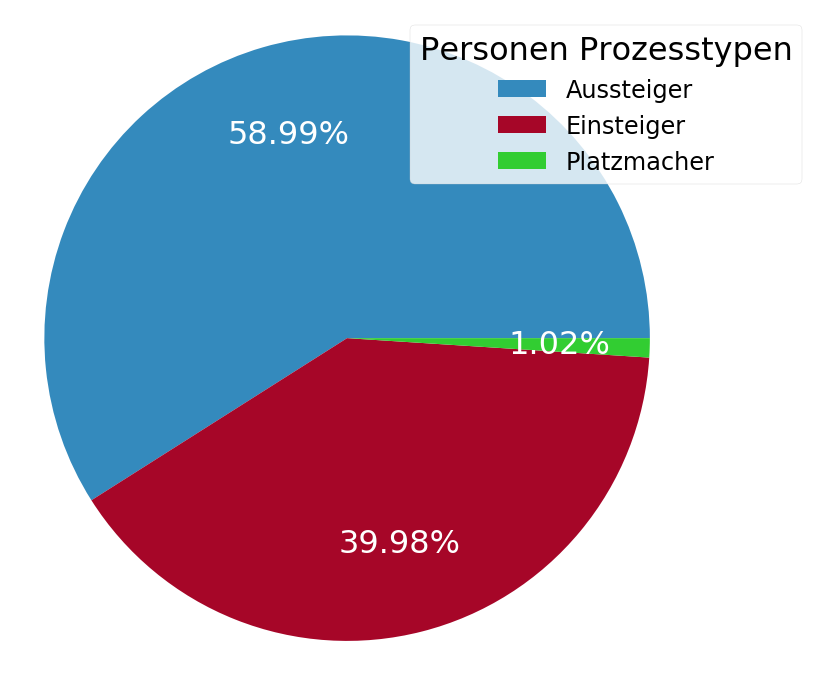
\includegraphics[width=0.6\textwidth]{pictures/data_evaluation/data_description/process_types.png}
	\caption{Anteil der Prozesstypen Aussteiger, Einsteiger und Platzmacher in den gesammelten Daten.}
	\label{fig:AnteileProzesstypen}
\end{figure}
Das Histogramm in \figurename\ref{fig:histAllePersonen} zeigt die Verteilung aller am Fahrgastwechsel teilnehmenden Personen. Hierbei geht es um die Anzahl der Einsteiger, Aussteiger und Platzmacher an jeder Tür.
\begin{figure}[H]
	\centering
		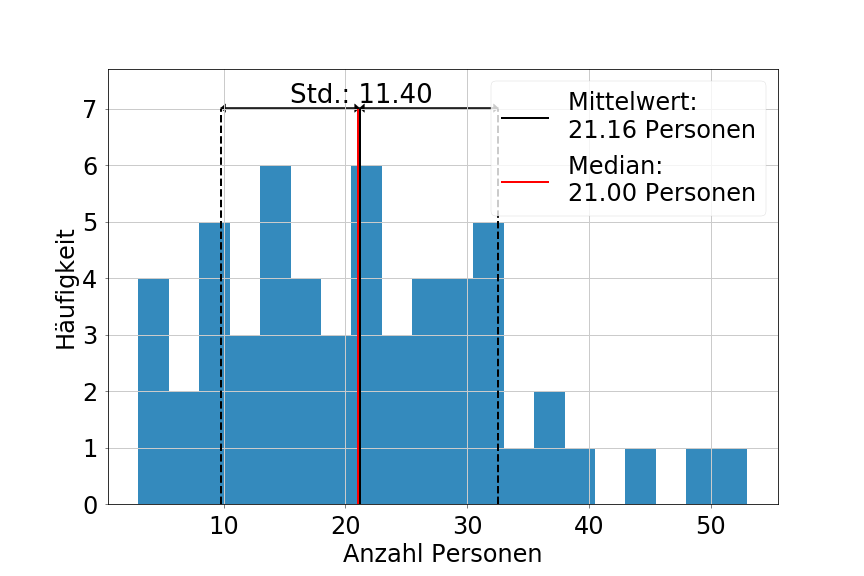
\includegraphics[width=0.7\textwidth]{pictures/data_evaluation/data_description/hist_persons.png}
	\caption{Histogramm der am Fahrgastwechsel beteiligten Personen, mit Später-Ein- und Später-Aussteigern, pro Tür mit einem Mittelwert von 21.16 Personen, einer Standardabweichung von 11.40 Personen und einem Median von 21.00 Personen.}
	\label{fig:histAllePersonen}
\end{figure}
Im Mittel sind es also \ca 21 Personen, die an einer Tür des Zuges ein-, aussteigen oder Platz machen. Auch der Median liegt bei 21 Personen und es besteht eine Standardabweichung von ungefähr 11 Personen.
\section{Fahrgastwechselzeiten} \label{Zeiten}
Mit Hilfe der Tabelle der Fahrgastwechselzeit (Ausschnitt \tablename \ref{tab:times}) beantworte ich nun die Forschungsfrage \ref{item:Fahrgastwechselzeiten} "`Kann die Fahrgastwechselzeit aus der Anzahl der Aus-, Einsteiger und Platzmacher abgeschätzt werden?"'. Um dies zu erreichen, führe ich eine lineare Regression mit der Methode der kleinsten Quadrate durch. Die erklärende Variable $x$ ist die Anzahl der am Prozess beteiligten Personen, und die Zielvariable $y$ ist die Fahrgastwechselzeit in Sekunden. Bevor ich die Regression durchführe, gebe ich zunächst ein Überblick über die Variablen. \cite{Fahrmeir.2009} nennen dies als ersten Schritt der Regressionsanalyse. \\
Für die Wechselzeiten untersuche ich nicht nur die Fahrgastwechselzeit, sondern auch die Kernwechselzeit (siehe \ref{Zeiten Tabelle}). Somit untersuche ich nicht nur den Zusammenhang der Anzahl der Fahrgäste und der Fahrgastwechselzeit, sondern auch der Zusammenhang zwischen der Anzahl der Kern-Personen (ohne Später-Ein- und Später-Aussteiger) und der Kernwechselzeit. Möchte man wissen, wie lange eine gewisse Anzahl an Personen für einen Fahrgastwechsel benötigen, so ist der Zusammenhang zwischen Kernwechselzeit und der Anzahl der Kern-Ein-, Kern-Aussteiger und Platzmacher interessant. Hier fällt der Störfaktor, dass Personen mit gewissem zeitlichem Abstand noch ein- oder aussteigen weg. Die Gesamtheit der Kern-Einsteiger, Kern-Aussteiger und Platzmacher werden im Nachfolgenden mit Kern-Personen bezeichnet, wobei Platzmacher doppelt gezählt werden. Möchte man jedoch betrachten, wie lange ein Zug durchschnittlich im Bahnhof verweilen muss, bis der Fahrgastwechsel beendet ist, ist der Zusammenhang zwischen Fahrgastwechselzeit und Anzahl der am Prozess beteiligten Personen interessanter. Im Nachfolgendem ist zu beachten, dass Platzmacher immer mit Faktor zwei gezählt werden, wenn es um die Wechselzeiten geht, da diese Personen sowohl aus- als auch einsteigen.\\ 
Für den ersten Überblick der Variablen bestimme ich die Lagemaße Mittelwert, Median und Standardabweichung und stelle die Verteilung mit Histogrammen grafisch dar (\cite{Fahrmeir.2009}). Für die Regressionsanalyse zeige ich das Histogramm der Kern-Personen (ohne Später-Ein- und Aussteiger) des Fahrgastwechsels, in \figurename \ref{fig:histPersonen}.
\begin{figure}[H]
	\centering
		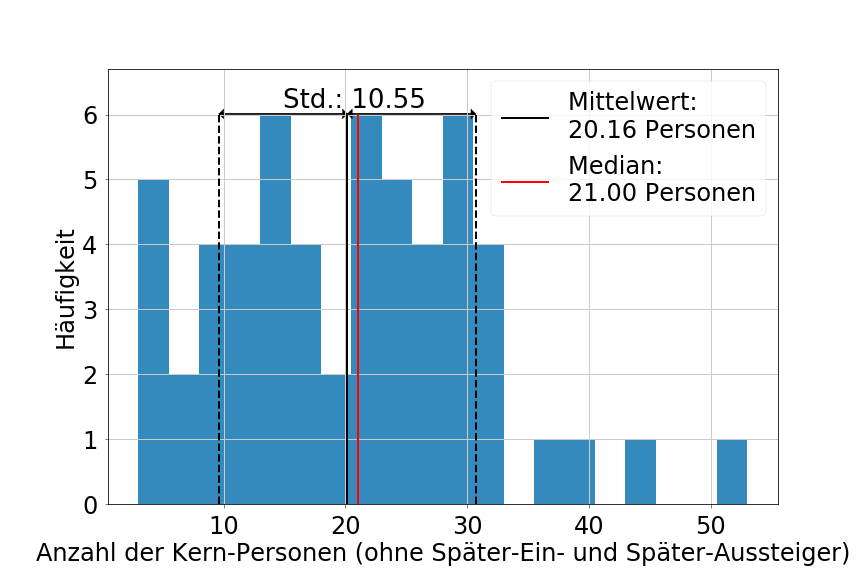
\includegraphics[width=0.7\textwidth]{pictures/data_evaluation/transferTime/hist_core_persons.png}
	\caption{Histogramm der am Fahrgastwechsel beteiligten Kern-Personen (ohne Später-Ein- und Später-Aussteiger) pro Tür mit einem Mittelwert von 20.16 Personen, einer Standardabweichung von 10.55 Personen und einem Median von 21 Personen.}
	\label{fig:histPersonen}
\end{figure}
Die Anzahl der gefilmten am Prozess beteiligten Kern-Personen schwankt zwischen 3 und 53 Personen, wobei die Anzahl der Kern-Personen in den meisten Videos zwischen 9 und 31 Personen liegt. Durchschnittlich sind es \ca 20 (20.16) Personen, die an einer Tür ein-, aussteigen oder Platz machen. Mehr als 32 Kern-Personen kommen in den Daten nur vereinzelt vor, weshalb für eine große Anzahl von Kern-Personen nur eine sehr ungenaue Aussage getroffen werden kann (\cite{Fahrmeir.2009}). Der Median des Datensatzes liegt bei 21 Kern-Personen pro Fahrgastwechsel. Zudem ist anzumerken, dass es sich um eine unsymmetrisch linksseitige Verteilung handelt.

Nicht nur die Kern-Personen der Beobachtungen werden hier betrachtet. Die Kernwechselzeit stelle ich ebenfalls in einem Histogramm dar (siehe \figurename \ref{fig:histTimes}). Hier ist zu erkennen, dass die Kernwechselzeit einen Mittelwert von 18.2 Sekunden besitzen. Der Median liegt hierbei bei 18.0 Sekunden und die Standardabweichung beträgt 8.3 Sekunden. 
\begin{figure}[H]
	\centering
		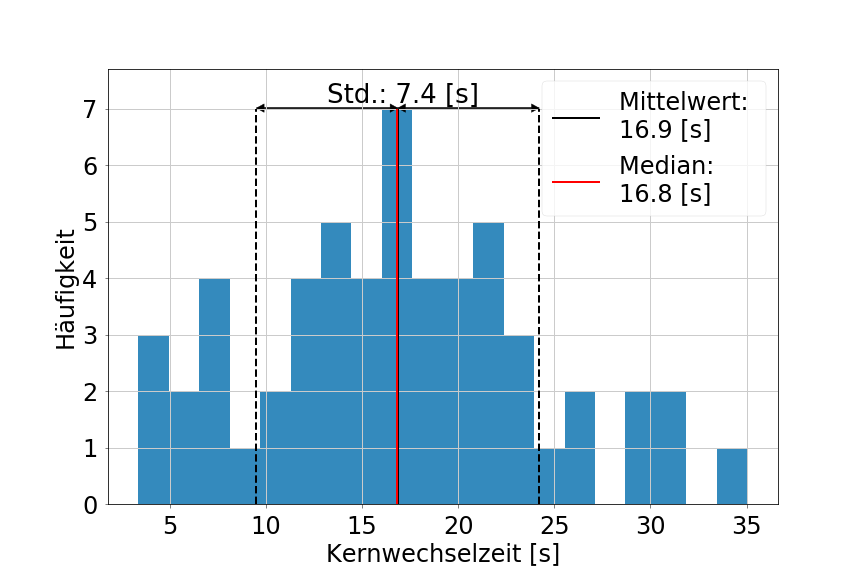
\includegraphics[width=0.7\textwidth]{pictures/data_evaluation/transferTime/hist_core_transfer_time.png}
	\caption{Histogramm der Kernwechselzeit, ohne Später-Ein- und Aussteiger, pro Tür mit einem Mittelwert von 18.2 Sekunden einem Median von 18.0 Sekunden und einer Standardabweichung von 8.3 Sekunden.}
	\label{fig:histTimes}
\end{figure}
Der Wert der benötigten Sekunden liegt zwischen 3.4 und 35.0 Sekunden. Die Verteilung ist hierbei symmetrischer als die der Kern-Personen, kann jedoch auch als eher linksseitig beschrieben werden.

Nachdem nun die Daten für die Kernwechselzeiten und Kern-Personen betrachtet wurden, stelle ich als nächstes die Histogramme für die Fahrgastwechselzeiten und Personen (mit Später-Ein- und Später-Aussteiger) vor. Das Diagramm der Personen ist in \figurename \ref{fig:histAllePersonen} zu sehen. \\
Die Anzahl der am Prozess teilhabenden Personen schwankt, wie bei den Anzahlen bei denen Später-Ein- und Später-Aussteigende nicht beachtet wurden, zwischen 3 und 53 Personen. Der Mittelwert der am Prozess beteiligten Personen erhöht sich durch das Einbeziehen späterer Fahrgäste jedoch von 20 auf \ca 21 (21.16) Personen. In den Daten der Personen liegt die überwiegende Mehrzahl der Anzahl an Fahrgästen zwischen 9 und 32 Personen. Auch hier gibt es wenige Prozesse, bei denen mehr als 32 Personen gezählt wurden. Genaue Aussagen können für diese Anzahlen nicht getroffen werden. Die Verteilung der Personen ist hierbei etwas weniger linksseitig als bei der Verteilung der Kern-Personen, sie ist jedoch auch unsymmetrisch links verteilt.

Nun wird zuletzt die Verteilung der Fahrgastwechselzeit betrachtet. Auch hierfür erstellte ich ein Histogramm, das in \figurename \ref{fig:histAllTimes} betrachtet werden kann.
\begin{figure}[H]
	\centering
	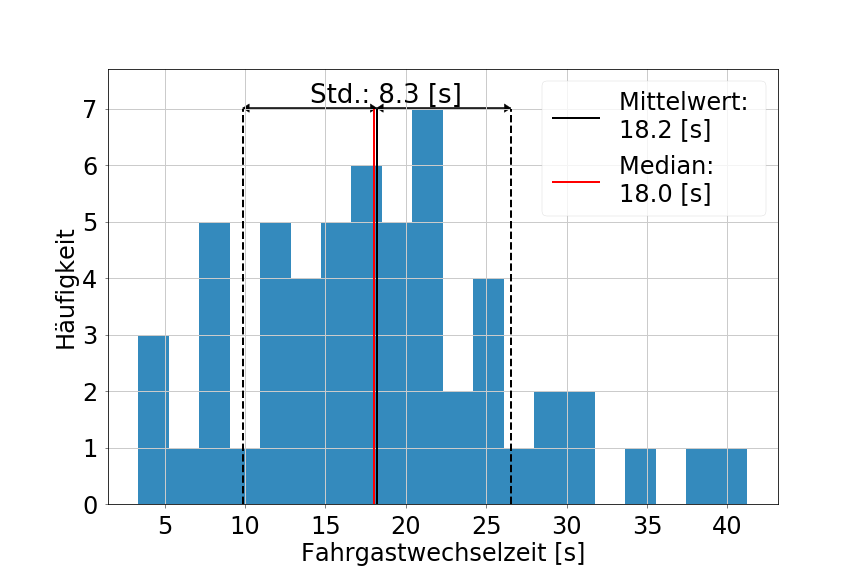
\includegraphics[width=0.7\textwidth]{pictures/data_evaluation/transferTime/hist_transfer_times.png}
	\caption{Histogramm der Fahrgastwechselzeiten pro Tür mit einem Mittelwert von 18.2 Sekunden einem Median von 18.00 Sekunden und einer Standardabweichung von 8.3 Sekunden.}
	\label{fig:histAllTimes}
\end{figure}
Die Werte für die Fahrgastwechselzeiten liegen zwischen 3.4 und 41.2 Sekunden. Für mehr als 32 Sekunden sind hierbei ebenfalls nicht sehr viele Daten gegeben, was auch hier zu Ungenauigkeiten in der Auswertung führen könnte. Die Verteilung ist ebenfalls leicht linksseitig.

Im nächsten Schritt untersuche ich nun der grafische Zusammenhang zwischen der Zielgröße und erklärenden Variable. Dadurch kann "`ein erster Überblick über die Art [...] und Stärke des Zusammenhangs gewonnen werden" (\cite{Fahrmeir.2009}: 13). \\
Zunächst betrachte ich die Kernwechselzeit in Abhängigkeit der Kern-Personenzahl. Wie auf \figurename \ref{fig:zusammenhangsAnalyse} zu erkennen ist, besteht ein annähernd linearer und monoton steigender Zusammenhang zwischen Anzahl der Kern-Personen und Kernwechselzeit. Ebenfalls zu erkennen ist, dass die Streubreite für größere Anzahlen an Kern-Personen sich erhöht.
\begin{figure}[H]
	\centering
		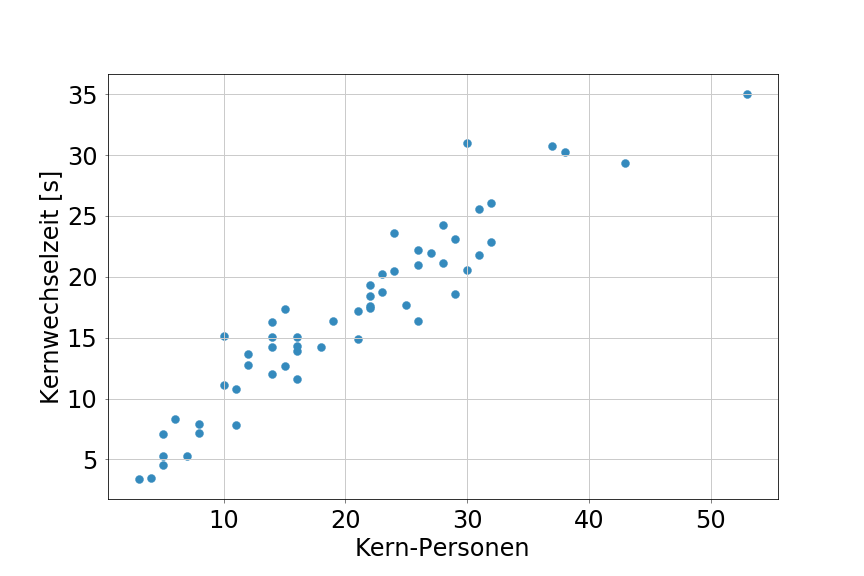
\includegraphics[width=0.7\textwidth]{pictures/data_evaluation/transferTime/core_coherence_analysis.png}
	\caption{Streudiagramm zwischen Anzahl der Kern-Personen (ohne Später-Ein- und Später-Aussteiger), und der Kernwechselzeit in Sekunden. Annähernd linearer und monoton steigender Zusammenhang.}
	\label{fig:zusammenhangsAnalyse}
\end{figure}
Nun stelle ich ebenfalls das Streudiagramm der Fahrgastwechselzeit in Abhängigkeit der Anzahl der Personen dar.
\begin{figure}[H]
	\centering
		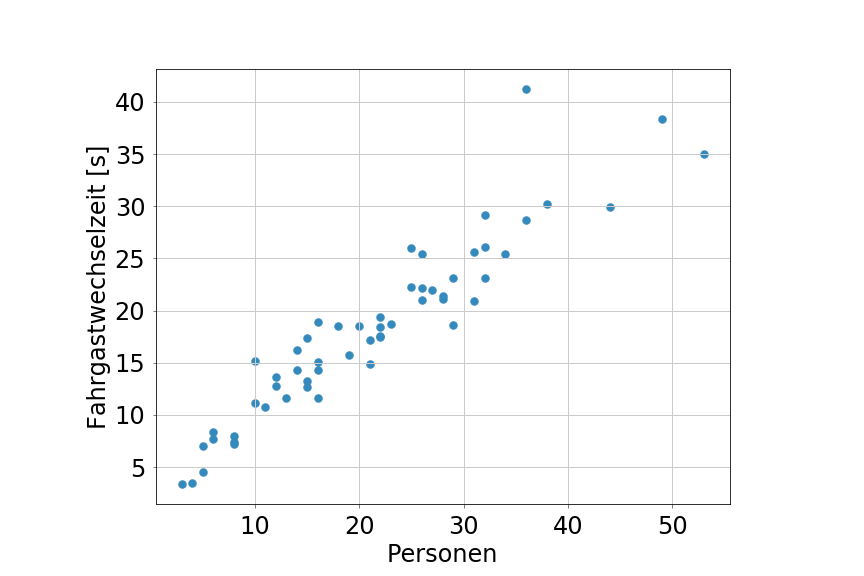
\includegraphics[width=0.7\textwidth]{pictures/data_evaluation/transferTime/coherence_analysis.png}
	\caption{Streudiagramm zwischen Anzahl der Personen, die am Fahrgastwechsel beteiligt sind inklusive Später-Ein- und Später-Aussteiger, und der Fahrgastwechselzeit in Sekunden. Annähernd linearer und monoton steigender Zusammenhang.}
	\label{fig:zusammenhangsAnalyseAlle}
\end{figure}
Auch in diesem Streudiagramm in \figurename \ref{fig:zusammenhangsAnalyseAlle} ist ein annähernd linearer monoton steigender Zusammenhang zu erkennen. Die Streubreite für große Anzahl der Personen ist hier noch höher als bei der Kernwechselzeit ohne Später-Ein- und Später-Aussteiger. 

Sowohl bei der Kernwechselzeit in Abhängigkeit der Kern-Personen als auch bei der Fahrgastwechselzeit in Abhängigkeit der Personen, ist ein linearer Zusammenhang erkennbar. Deshalb führe ich für beide Zusammenhänge jeweils eine lineare Regression durch. Wie schon erwähnt, ist die Zielvariable jeweils die entsprechende Zeit (Fahrgastwechselzeit und Kernwechselzeit) und die Kovariable die entsprechende Anzahl an Personen (mit und ohne Spätere). \\
In Anhang \ref{append:LinReg} wird das Vorgehen zur linearen Regression erläutern.

Um die lineare Regression mit \texttt{Python} durchführen zu können, wird die Bibliothek \texttt{statsmodels.formula.api} verwendet. Mit der \texttt{ols} Methode dieser Bibliothek kann ein Modell erstellt werden, welches dieser mit einem R-Style Formular übergeben wird. Dabei verwendet \texttt{statsmodel} das \texttt{patsy} Packet, welches das Formulare und Daten, in Matrizen umwandelt, die der Modellanpassung dienen. Wendet man auf das Ergebnis der \texttt{ols} Methode dann die \texttt{fit} Methode an, so wird das Modell angepasst und  man erhält man ein \texttt{RegressionResultWrapper} Objekt. In diesem Objekt sind die Ergebnisse der Regression zusammengefasst. \\
Für die lineare Einfachregression wird die Regression folgendermaßen aufgerufen:
\begin{lstlisting}[language=Python]
import statsmodels.formula.api as smf

res_lin = smf.ols(formula="time ~ persons", data=data_time).fit()
\end{lstlisting}
Die Variable \texttt{time} und \texttt{persons} die durch das R-Style Formular übergeben werden sind \texttt{Arrays}. \texttt{Time} enthält die gemessenen Fahrgastwechselzeiten und \texttt{persons} die Anzahlen der Personen, die am Fahrgastwechsel beteiligt sind. Die Variable \texttt{data\_time} ist der \texttt{Dataframe} der Tabelle der Fahrgastwechselzeiten. Das Ergebnis \texttt{res\_lin} ist ein \texttt{RegressionResultWrapper}, der unter anderem die Schätzwerte enthält.

Bei der Zusammenhangsanalyse habe ich festgestellt, dass die Daten, sowohl die mit als auch die ohne Spätere, einen annähernd linearen Zusammenhang besitzen. Deshalb führe ich für die Daten ohne Später-Ein- und Später-Aussteiger nun eine lineare Einfachregression durch.\\
Das Modell für die Zielvariable $Kernwechselzeit$ in Abhängigkeit der Kovariable $Kern\text{-}Personen$ (Einsteiger, Aussteiger und Platzmacher ohne Spätere) ist für die lineare Einfachregression also:
\begin{equation}
Kernwechselzeit_i = \beta_0 + \beta_1 \cdot Kern\text{-}Personen_i + \varepsilon_i
\label{eq:LinFahrgastwechselzeit}
\end{equation} 
Die Methode \texttt{fit()} von \texttt{Python} gibt, unter anderem, für die Funktion \ref{eq:LinFahrgastwechselzeit} die Schätzparameter $\hat{\beta_0}$ und $\hat{\beta_1}$ zurück. In diesem Fall ergibt sich für die lineare Regression: $\hat{f}(Kern\text{-}Personen) = \hat{\beta_0} + \hat{\beta_1} \cdot Kern\text{-}Personen$. Diese kann zur Prognose der $Kernwechselzeit$ verwendet werden.
Die von \texttt{Python} zurückgebenden Schätzwerte sind: $\hat{\beta_0}=3.55$ und $\hat{\beta_1}=0.66$. Das Streudiagramm mit der Schätzfunktion $\hat{f}$ und dem Konfidenzintervall der Funktion kann in \figurename \ref{fig:LinReg} betrachtet werden.
\begin{figure}[H]
	\centering
		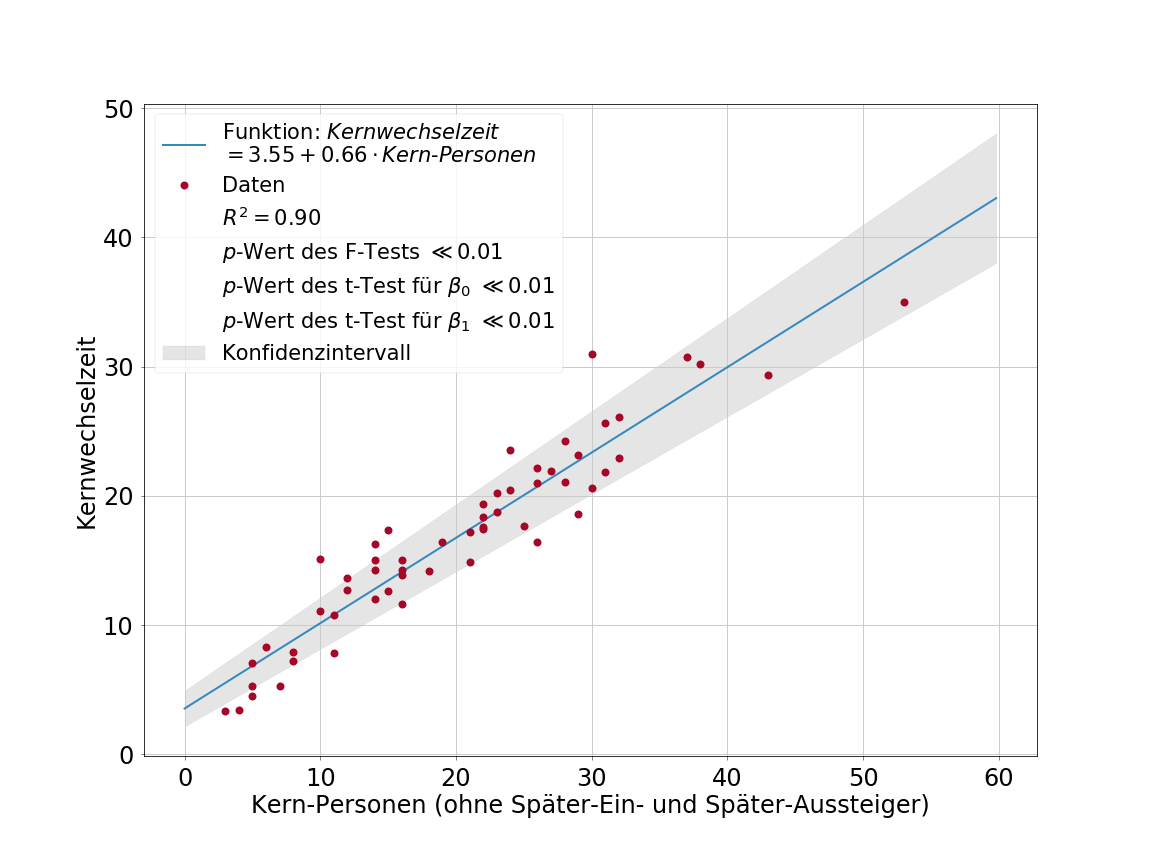
\includegraphics[width=0.7\textwidth]{pictures/data_evaluation/transferTime/lin_core_transfer_time.png}
	\caption{Streudiagramm und lineare Regression der Anzahl der Kern-Personen ($x$) und Kernwechselzeit in Sekunden ($y$) und der geschätzten Funktion: $y = 3.55 + 0.66 \cdot x$, mit dem 95\% Konfidenzintervall.}
	\label{fig:LinReg}
\end{figure}
Nach der Anwendung der linearen Einfachregression überprüfe ich nun, wie gut die Schätzfunktion für die Daten geeignet ist. Dabei ziehe ich das Bestimmtheitsmaß, welches mit $R^2$ bezeichnet wird, heran. Das Bestimmtheitsmaß misst die Güte der Anpassung an die Daten. Auch die Erklärung des Bestimmtheitsmaßes kann im Anhang in \ref{append:rsquared} nachgelesen werden. \\
Die \texttt{fit} Methode gibt das Bestimmtheitsmaß in ihrem Ergebnis zurück. Für die lineare Einfachregression ergibt sich $R^2=0.9$. Dieser Wert liegt somit nah an der 1. Es ist also zu vermuten, dass die Anpassung an die Daten sehr gut ist. 

Es ist jedoch für die Beurteilung des Modells nicht nur wichtig, die Anpassung an die Daten zu betrachten. Zudem führe ich noch statistische Tests durch, um die Regressionsparameter zu überprüfen. "`Voraussetzung für die Konstruktion von (exakten) Tests [...] ist die Gültigkeit der Normalverteilungsannahme der Störgrößen. [Wir setzen] also zunächst unabhängige und identisch verteilte Störgrößen $\varepsilon_i \sim N(0,\sigma^2)$ voraus."'(\cite{Fahrmeir.2009}:111) Die Tests sind jedoch relativ robust gegenüber geringfügigen Abweichungen von der Normalverteilung, weshalb ich im Folgenden annehme, dass die Störgrößen normalverteilt sind (\cite{Fahrmeir.2009}).\\
Im folgenden Abschnitt führe ich nun ein Test auf die Signifikanz der Einflussvariablen durch. Die statistischen Hypothesen für diesen Test lauten:
$$ H_0 : \beta_j = 0 \ \ \text{gegen} \ \ H_1: \beta_j \neq 0. $$
Das betrachtet Testprobleme kann, wenn die Variablen einzeln betrachtet werden, als Spezialfälle des Tests allgemeiner linearer Hypothesen
$$H_0: \boldsymbol{C}\boldsymbol{\beta} = \boldsymbol{d} \ \ \text{gegen} \ \ H_1: \boldsymbol{C}\boldsymbol{\beta} \neq \boldsymbol{d}$$
aufgefasst werden. Wobei $\boldsymbol{C}$ ein $r \times p$ Matrix ist (\cite{Fahrmeir.2009}). Dieser Test wird als F-Test bezeichnet und zeigt die Signifikanz der gesamten Regression an. Die Nullhypothese wäre hier also der Fall, dass alle Schätzparameter, abgesehen von der Konstante, gleich null sind. Die Nullhypothese wird abgelehnt, falls die Teststatistik größer ist als das $(1-\alpha)$-Quantil der entsprechenden F-Verteilung, wobei $\alpha$ das Signifikanzniveau bezeichnet (\cite{Fahrmeir.2009}). Die Definition des Signifikanzniveaus kann im Anhang in \ref{append:Signifikanzniveau} nachgelesen werden. \\
Neben der eben genannten Vorgehensweise, mit dem Vergleich dem kritischen Wert aus der F-Verteilung, gibt es jedoch auch die Möglichkeit, statistische Tests über die sogenannten $p$-Werte durchzuführen. Anstatt die Prüfgröße mit einem bestimmten kritischen Wert zu vergleichen, um über die Ablehnung der Nullhypothese zu entscheiden, vergleicht man den $p$-Wert direkt mit dem vorgegebenen Signifikanzniveau $\alpha$. Der $p$-Wert gibt nämlich gerade die Wahrscheinlichkeit an, unter $H_0$ den beobachteten Prüfgrößenwert zu erhalten. Die Nullhypothese ist also dann zu verwerfen, falls der $p$-Wert kleiner ist als $\alpha$ (\cite{Fahrmeir.2011}).

Das Ergebnis der Regression von \texttt{statsmodel} gibt eben diesen $p$-Wert für die F-Statistik an. Um also zu Testen ob die Schätzgrößen zusammenwirkend Signifikant sind, betrachte ich eben diesen Wert. Zunächst lege ein Signifikanzniveau von $\alpha = 0.01$ fest. Der berechnetet $p$-Wert des F-Test für das Modell der lineare Einfachregression ist $ \ll 0.01$. Die Nullhypothese wird deshalb abgelehnt. Es ist also davon auszugehen, dass die Schätzparameter zusammenwirkend signifikant sind.

Neben der Signifikanz der Regression, teste ich nun auch die Signifikanz der einzelnen Einflussvariablen. Diese Tests werden als t-Tests bezeichnet und besitzen die Hypothesen:
$$ H_0:\beta_j = 0 \ \ \text{gegen} \ \ H_1: \beta_j \neq 0 \ \ j = 0, ..., p$$
Beim einem t-Test ist der kritische Wert für den Ablehnungsbereich der Nullhypothese durch das $(1-\alpha/2)$-Quantil der $t$-Verteilung gegeben.

Auch auf die $p$-Werte der t-Tests kann im Ergebnis von \texttt{Python} zugegriffen werden. Hierbei verwende ich ebenfalls ein Signifikanzniveau von $\alpha = 0.01$. Der $p$-Wert des t-Tests der Konstante ist $\ll 0.01$. Die Nullhypothese kann damit abgelehnt werden, und es kann gesagt werden das der Schätzparameter $\beta_0$ einen signifikanten Einfluss besitzt. Da der F-Test für die lineare Einfachregression dem t-Test des Parameters $\beta_1$ entspricht, und diese für den F-Test schon abgelehnt wurde, kann auch hier gesagt werden, dass die Nullhypothese abgelehnt wird, und der Schätzparameter einen Einfluss auf die Regression besitzt.

Durch die durchgeführten Tests und die Betrachtung des Bestimmtheitsmaß kann angenommen werden, dass das Modell der linearen Einfachregression die Daten sehr gut beschreibt. Da der geschätzte Wert der Kernwechselzeit für 0 Personen jedoch schon bei 3.55 Sekunden liegt, was unplausibel ist, und die Daten mit wenigen Kern-Personen unter der Kurve verbleiben, kam mir die Idee ein Modell anzuwenden, welches sowohl einen logistischen als auch eine linearen Teil enthält.

Dazu führe ich ebenfalls eine lineare Regression mit \texttt{statsmodel} durch. Jedoch ist hier das Modell:
\begin{equation}
Kernwechselzeit = \beta_0 + \beta_1 \cdot \log(Kern\text{-}Personen) + \beta_2 \cdot Kern\text{-}Personen
\end{equation}
Sieht man sich nur das Bestimmtheitsmaß der Regression an, so scheint diese Funktion auch zu den Daten zu passen. Der $R^2$-Wert hat sich für das Modell mit logarithmischem Anteil mit einem Wert von $0.9$ nicht verschlechtert. Auch der $p$-Wert bleibt bei der F-Statistik unverändert $\ll 0.01$. Das Zusammenspiel der Schätzwerte hat also einen Einfluss. Betrachtet man jedoch die $p$-Werte der t-Statistik für die einzelnen Schätzwerte, so wird deutlich, dass die lineare Einfachregression besser für die gegeben Daten geeignet ist, da die $p$-Wert von $\beta_1$ mit $0.02$ und $\beta_0$ mit $0.41$ das Signifikanzniveau überschreiten. Deshalb wird Nullhypothesen für $\beta_1$ und $\beta_0$ angenommen, die Parameter haben höchst wahrscheinlich keinen Einfluss auf die Regression.

Die Fahrgastwechselzeit kann also mit der Funktion 
\begin{equation}
f(Kern\text{-}Personen) = 3.55 + 0.66 \cdot Kern\text{-}Personen
\end{equation}  
durch die Anzahl der am Fahrgastwechsel beteiligten Personen abgeschätzt werden. Damit ist zu sagen das die Kernwechselzeit sich pro Kern-Person um etwa $0.66$ Sekunden erhöht.

Nachdem nun ich die Kernwechselzeit für die beteiligten Kern-Personen ohne Später-Ein- oder Später-Aussteiger mit der linearen Einfachregression geschätzt habe, führe ich nun auch eine lineare Einfachregression für die Fahrgastwechselzeit durch. Hierbei untersuche ich den Zusammenhang zwischen den am Fahrgastwechsel beteiligten Personen, mit Später-Ein- und Später-Aussteigern, als erklärende Variable $x$, und der Fahrgastwechselzeit als Zielvariable $y$. Die Zielvariable gibt dann die Zeit an, welche ein Zug voraussichtlich am Bahnhof verbringen muss, wenn eine bestimmte Anzahl an Personen den Zug verlassen und betreten wollen. Diese Schätzung dient eher der Fahrplan-Planung als die Vorangegangene, welche nur besagte wie lange Personen für einen Fahrgastwechsel benötigen, ohne dabei zu berücksichtigen, dass manche Personen erst später an den Zug gelangen oder aus ihm aussteigen. Das "`später Einsteigen"' und "`später Aussteigen"' Verhalten wird an 35.71 \% der Türen gezeigt.

Auch hier habe ich bei der Zusammenhangsanalyse festgestellt, dass der Zusammenhang annähernd linear ist. Somit führe ich auch hier eine lineare Einfachregression, diesmal mit dem Modell
\begin{equation}
Fahrgastwechselzeit = \beta_0 + \beta_1 \cdot Personen
\end{equation}
durch. Die Variable $Fahrgastwechselzeit$ stellt hierbei die Fahrgastwechselzeit für alle Personen und die Variable $Personen$ die Anzahl der Personen inklusive Späterer dar.
\begin{figure}[H]
	\centering
		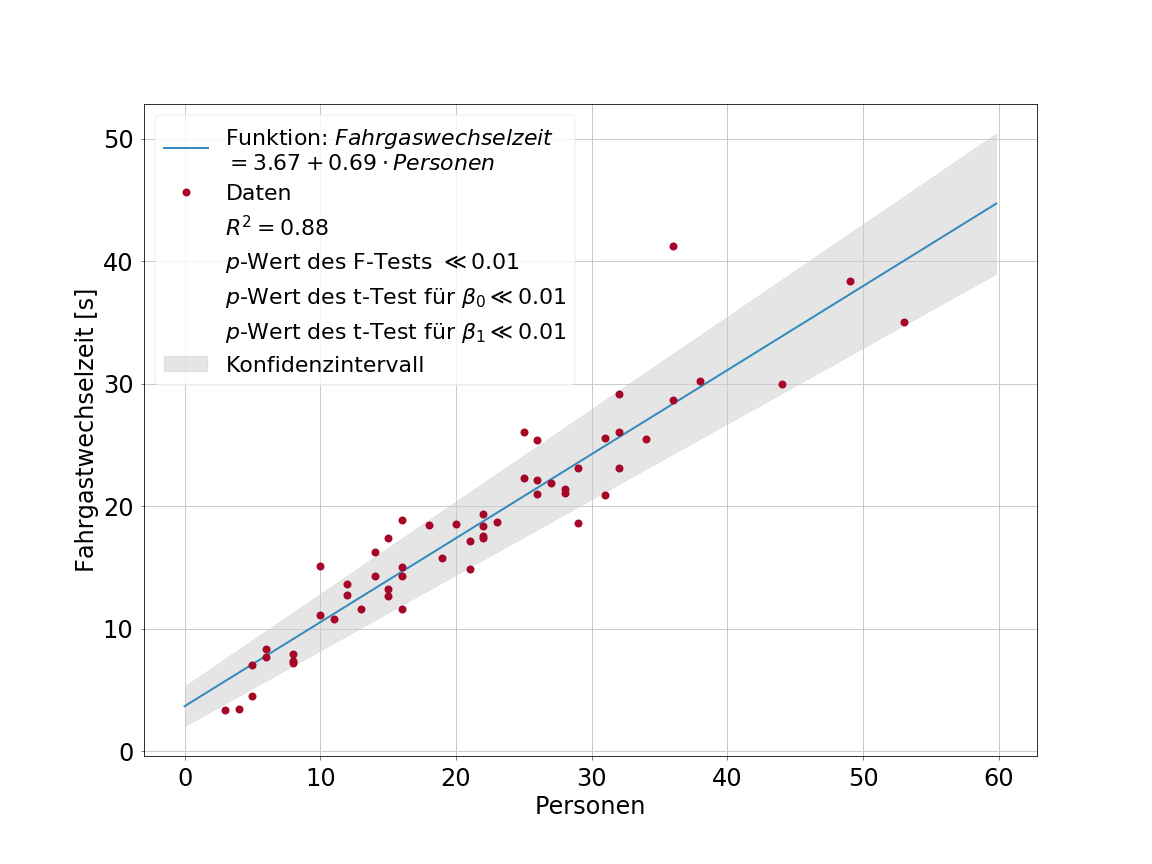
\includegraphics[width=0.7\textwidth]{pictures/data_evaluation/transferTime/lin_transfer_time.png}
	\caption{Lineare Regression zwischen Anzahl der Personen die am Fahrgastwechsel beteiligt sind ($x$) und der Fahrgastwechselzeit in Sekunden ($y$) und der geschätzten Funktion, $y= 3.67 + 0.69 \cdot x$, sowie dem 95\% Konfidenzintervall.}
	\label{fig:LinRegAlle}
\end{figure}
Die von \texttt{Python} zurückgebenden Schätzwerte sind hier: $\hat{\beta_0}=3.67$ und $\hat{\beta_1}=0.69$. Das Streudiagramm mit der Schätzfunktion und dem Konfidenzintervall der Funktion kann in \figurename \ref{fig:LinRegAlle} betrachtet werden.
Die Schätzparameter haben sich hierbei, im Gegensatz zu denen im Modell ohne spätere Personen, also nur etwas erhöht. Die Steigung der Kurve erhöht sich hier von $0.66$ auf $0.69$ und die Konstante der Gerade von $3.55$ auf $3.67$. \\
Das Bestimmtheitsmaß verringerte sich durch die Beachtung der Späteren jedoch auf $0.889$ dieser Wert gibt immer noch eine gute Angepasstheit an die Daten an, zeigt jedoch auch, dass die Schätzung für die Zielgröße wahrscheinlich etwas ungenauer ist als bei der Aussparung der Personen die erst später zum Fahrgastwechsel hinzustoßen. Wie bei der vorangegangenen Untersuchung stimmen auch bei dieser linearen Einfachregression die $p$-Werte für die F-Statistik und die t-Statistik des $\beta_1$ überein, weshalb hier nur die t-Tests durchgeführt werden. Das Signifikanzniveau $\alpha$ besitzt weiterhin den Wert 0.01. Für die Konstante $\beta_0$ ergibt sich für den t-Test ein $p$-Wert der $\ll 0.01$ ist. Die Nullhypothese wird abgelehnt und es kann somit angenommen werden, dass diese Konstante Einfluss besitzt. Auch der $p$-Wert der $\beta_1$ Schätzung ist für den t-Test $\ll 0.01$. Auch hier kann ein Einfluss des Schätzparameters angenommen werden, da die Nullhypothese abgelehnt wurde.

Auch für diesen Zusammenhang versuche ich noch einmal ein Modell mit logarithmischem Anteil anzuwenden. Weil die $p$-Werte der t-Statistik jedoch über dem Signifikanzniveau liegen, wurde auch für die Fahrgastwechselzeit das Modell mit der Geraden angenommen.

Die Funktion 
\begin{equation}
f(Personen) = 3.67 + 0.69 \cdot Personen 
\end{equation}  
kann die Fahrgastwechselzeit also gut abschätzen. Damit ist anzumerken, dass sich die Fahrgastwechselzeit für eine Person mehr um ungefähr 0.69 Sekunden erhöht, und damit nur um 0.03 Sekunden mehr als bei der Kernwechselzeit.

Mit diesen Funktionen können die Wechselzeiten (Kernwechselzeit oder Fahrgastwechselzeit) im Normalfall abgeschätzt werden. Somit kann die Forschungsfrage \ref{item:Fahrgastwechselzeiten} mit Ja beantwortet werden. Mit den Funktionen kann sowohl die wahrscheinliche Zeit für den Fahrgastwechsel als auch die benötigte Haltezeit der U-Bahn, im Standardfall, abgeschätzt werden. Dies Abschätzungen könnten in die Planung von U-Bahn-Stationen und Fahrplänen einfließen. Ein weiterer Verwendungszweck könnte das Einsetzen dieser Funktion bei der Modellvalidierung sein. Wird ein Modell basierend auf dem Entscheidungsprozess erstellt und simuliert, könnten die durch Simulationen erhobenen Fahrgastwechselzeiten mit diesen Funktionen verglichen, und so eine Aussage über die Plausibilität des Modells gemacht werden. Die Ergebnisse können zudem für die Kalibrierung des Modells verwendet werden. 

Die Auswertungen der Fahrgastwechselzeiten mit \textsf{Jupyter Notebook} können im Zusatzmaterial in der Datei \texttt{TransferTime.ipynb} betrachtet werden.
\section{Gruppen} \label{Gruppen}
Im Simulationsprogramm der Firma accu:rate existiert bereits ein Modell für Gruppenverhalten. Da das Verhalten von Gruppen eine Simulation beeinflusst, beschreibe ich in diesem Abschnitt die Auswertung der Gruppentabellen (\tablename \ref{tab:groupsAS}, \tablename \ref{tab:groupsES} und \tablename \ref{tab:groupsPM}). Durch die Auswertung dieser Tabellen beantworte ich die Forschungsfrage \ref{item:Goupsize} "`Kann aus dem Filmmaterial gewonnen werden, welche Gruppengrößen im Fahrgastwechsel auftreten und wie viel Prozent der Personen sich in einer Gruppe mit einer bestimmten Größe befinden?"'.

In der Software von accu:rate werden in einer Tabelle, die in einer Simulation vorkommenden Gruppengrößen, mit dem zugehörigen prozentualen Anteil der Agenten, welche in einer Gruppe dieser Größe sind, angegeben. Deshalb stelle die beobachteten Anteile von Personen in den Gruppen durch ein Kuchendiagramm (\figurename \ref{fig:AnteileGruppen}) dar.
\begin{figure}[H]
	\centering
		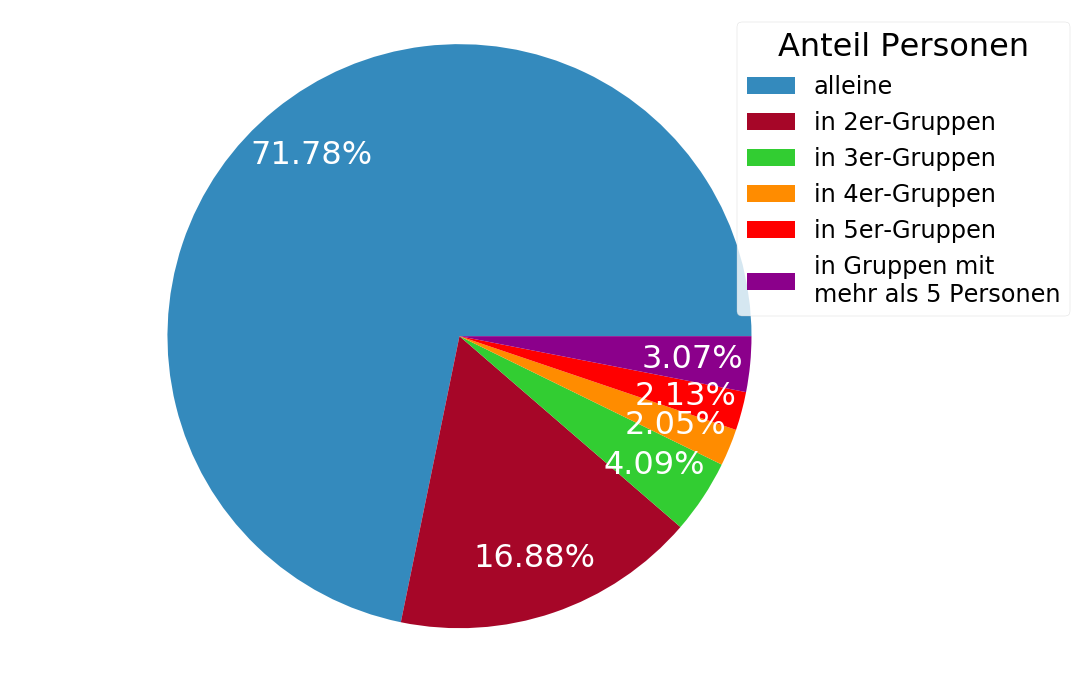
\includegraphics[width=0.7\textwidth]{pictures/data_evaluation/groups/groups.png}
	\caption{Kuchendiagramm der Anteile der Personen, die in einer Gruppe mit einer gewissen Gruppengröße beobachtet wurden.}
	\label{fig:AnteileGruppen}
\end{figure}
Gruppen erkenne ich durch Verhaltensweisen, wie das Sprechen mit oder warten auf andere Mitglieder der Gruppe. Bei den prozentualen Anteilen unterscheide ich nicht zwischen den Prozesstypen Einsteigern, Aussteigern und Platzmachern, da der Prozesstyp keine Auswirkung darauf hat, welcher Gruppengröße eine Person angehört. Da in den Tabellen nur die Anzahl der Gruppe mit einer gewissen Größe in einem Video angegeben ist und nicht die Anzahl der Personen in dieser Gruppe, wurde für die Auswertung die Gruppenstärke mit der Anzahl der vorkommenden Gruppen multipliziert. 

Die meisten beobachteten Fahrgäste sind alleine unterwegs. In dieser Art von "`Gruppe"' ist ein Anteil 71.78\%. Der nächstgrößere Anteil an Fahrgästen befindet sich, mit einem Anteil von 16.88\%, in Gruppen von zwei Personen. Gruppen mit drei Personen machen einen Anteil von 4.09\% aus. 4-er und 5-er Gruppen besitzen nur noch einen Anteil von \ca 2\% (2.05\% für 4-er-, 2.13\% für 5-er-Gruppen).Der letzte in der Grafik aufgeführte Anteil, ist der Anteil der Personen die in Gruppen mit einer Gruppenstärke von mehr als 5 Personen sind. Diese Bezeichnung führte ich ein, da im Filmmaterial zwar Gruppen mit mehr als 5 Personen erkennbar sind, es jedoch schwierig ist, eine allgemein geltende Behauptung zu deren Gruppengrößen und Anteilen anzustellen. So filmte ich \zB eine Gruppe von 11 Personen, es gibt für diese Größe jedoch nur eine einzige Gruppe, die von mir entdeckt wurde. Zudem beobachtete ich keine 10-er, 9-er oder 8-er Gruppen. Es ist jedoch zu vermuten, dass im realen Leben auch Gruppen mit einer Größe von 8, 9, 10 oder mehr als 11 Personen vorkommen. Deshalb wähle ich den Ausdruck von mehr als 5 Personen, da bei einem größeren Datensatz hier wahrscheinlich noch andere Gruppenstärken auftreten. Diese Art der "`Gruppe"' besitzt einen Anteil von 3.07\%.

Die gesammelten Daten geben einen groben Überblick über die unterschiedlichen Gruppenstärken. Die Forschungsfrage, "`Kann aus dem Filmmaterial gewonnen werden, welche Gruppengrößen im Fahrgastwechsel auftreten und wie viel Prozent der Personen sich in einer Gruppe mit einer bestimmten Größe befinden?"', würde ich jedoch nicht mit Ja beantworten. Wie ich beschrieben habe, ist nicht klar, ob mit den gesammelten Daten alle Gruppengrößen des realen Lebens beobachtet wurden. Zudem können die Daten so nicht in das Modell von accu:rate eingefügt werden. Das Modell von accu:rate möchte alle auftretenden Gruppengrößen und deren genauen Prozentualen Anteil. Für einzelne Personen, sowie 2-er und 3-er Gruppen können die Aussagen noch getroffen werden. Bei Personen, die in einer Gruppe von mehr als 5 Personen sind, kann dies jedoch nicht mehr gewährleistet werden. Wenn die Auswertung meiner Beobachtungen in das Modell mit einfließen sollen, müsste dieses angepasst werden. Es müsste die Möglichkeit geben eine Gruppenstärke anzugeben, die beschreibt, dass es sich um eine Gruppe handelt, die aus mehr als 5 Personen bestehen. Die Gruppenstärke könnte dann zufällig gewählt werden. Ein weiteres Problem mit diesen Daten ist, dass argumentiert werden könnte, dass nicht alle Gruppen erkannt wurden. Ich stimme diesem Argument zu. Ich behaupte jedoch, dass alle relevanten Gruppen erkannt wurden. Relevante Gruppen sind für mich Gruppen, die Gruppenverhalten zeigen.

Die Auswertung der Gruppen mit \textsf{Jupyter Notebook} kann im Zusatzmaterial in der Datei \textsl{GroupSize.ipynb} gefunden werden.
\section{Verhaltensweisen und Merkmale} \label{Verhalten}
Nach den Gruppengrößen und Wechselzeiten untersuche ich nun auch die Verhaltensweisen und Merkmale der beobachteten Personen. Dabei werte ich die bereits beschriebene Tabelle der Verhaltensweisen und Merkmale, \tablename \ref{tab:Vehalten}, aus. Durch dieses Vorgehen beantworte ich die Forschungsfragen \ref{item:Verhalten,Verhalten} "`Beeinflussen die Verhaltensweisen "`früher Einsteigen"' und "`Im Weg Stehen"' die Fahrgastwechselzeiten?"' und \ref{item:Vehalten,Merkmale} "`Beeinflussen die Merkmale "`sperrig"', "`langsam"' und "`abgelenkt"' der Fahrgäste die Fahrgastwechselzeit?"'. Bevor ich darauf eingehe, ob und wie sich diese Merkmale und Verhaltensweisen auf die Fahrgastwechselzeit auswirken, betrachte ich zunächst, wie oft diese beobachtet wurden. Ich gehe so vor, um einschätzen zu können, ob die Verhaltensweisen und Merkmale überhaupt relevant sind. Beobachte ich diese nur in sehr wenigen Fällen, so sind sie für die Modellierung uninteressant. Zu diesem Zweck erstelle ich ein Balkendiagramm, welches in \figurename \ref{fig:BalkenVerhalten} zu sehen ist. Die Balken stellen hierbei den prozentualen Anteil der Türen da, an denen das entsprechende Verhalten oder Merkmal gezeigt wurde.
\begin{figure}[H]
	\centering
		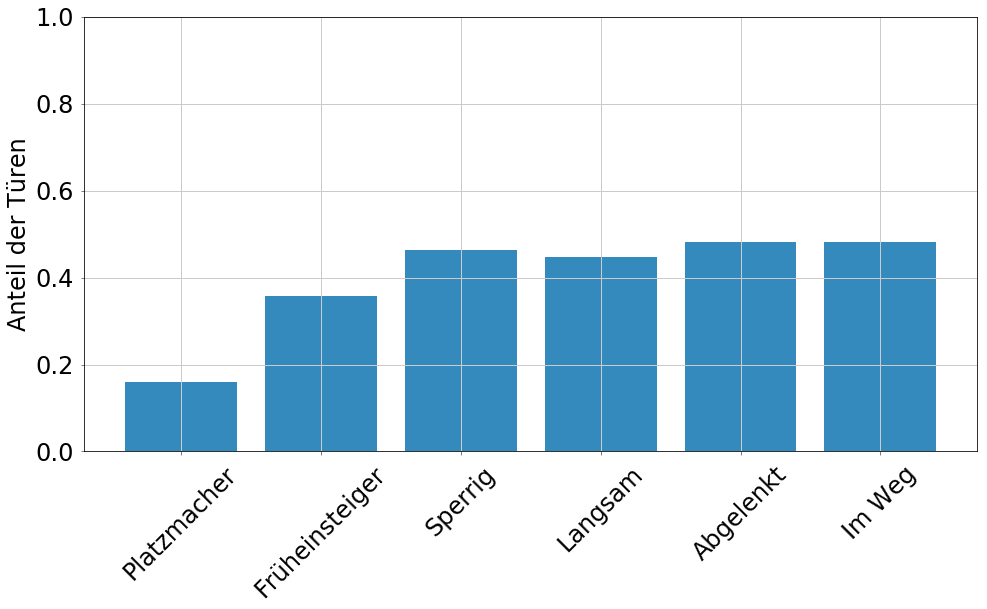
\includegraphics[width=0.8\textwidth]{pictures/data_evaluation/behavior/counts_behavoirs.png}
	\caption{Balkendiagramm der prozentualen Anteile von Verhaltensweisen und Merkmalen. Der prozentuale Anteil bezieht sich hierbei auf den Anteil der gefilmten Türen, an denen das entsprechende Verhalten oder Merkmal beobachtet wurde.}
	\label{fig:BalkenVerhalten}
\end{figure}
Zu erkennen ist, dass alle Verhaltensweisen und Merkmale in weniger als 50 \% der Videos gezeigt wurden. Abgesehen vom Verhalten "`Platz machen"' liegen diese jedoch alle knapp unter oder über 40 \%. Ein Verhalten, welches an \ca 40 \% der Türen gezeigt wird, ist meinem Empfinden nach relevant und sollte, falls es ebenfalls einen Einfluss auf die Fahrgastwechselzeit besitzt, modelliert werden. Um eine Entscheidung, darüber zu treffen ob die Verhaltensweisen "`früher Einsteigen"' und "`im Weg Stehen"', sowie die Merkmale "`sperrig"', "`langsam"' und "`abgelenkt"' für das Modell relevant sind, wird ihr Einfluss auf die Zeit untersucht. Zunächst soll jedoch noch auf die Verhaltensweise "`Platz machen"' eingegangen werden. Platzmacher treten nur an 16.07 \% der Türen auf und liegen damit deutlich unter 40 \%. Wie jedoch schon erwähnt stellen sie einen wichtigen Teil des Fahrgastwechsels dar, da sie sowohl ein- als auch aussteigen müssen, um Platz zu machen. Dass diese Verhaltensweise nur selten auftritt, ist zudem damit zu erklären, dass Platzmacher erst notwendig werden, wenn viele Personen im Wagon sind \bzw am Fahrgastwechsel beteiligt sind. Sind nur wenige Personen im Wagon und somit nur wenig Aussteiger vorhanden, können Fahrgäste ungehindert aussteigen und Platzmacher werden nicht benötigt. Ob es einen Zusammenhang zwischen der Anzahl der Aussteiger und dem Auftreten von Platzmachern gibt, untersuche ich nach der Untersuchung des zeitlichen Einflusses der andere Verhaltensweisen und Merkmale.

Um die Unterschiede der Fahrgastwechselzeit für die genannten Verhaltensweisen und Merkmale zu überprüfen, verwende ich die Fahrgastwechselzeit pro Person. Durch die Verwendung der Fahrgastwechselzeit pro Person wird verhindert, dass die Zeit des Fahrgastwechsels für eine großen Anzahl von Fahrgästen mit der für eine kleinen Anzahl von Personen verglichen wird. Um die Fahrgastwechselzeit pro Person zu gewinnen, erhob ich jedoch nicht die Zeit für jede Person in einem Video. Diese Zeit berechne ich, indem ich die Fahrgastwechselzeit durch die Anzahl der am Fahrgastwechsel beteiligten Personen (mit doppelt gezählten Platzmachern) teile. \\
Durch die Verwendung der Fahrgastwechselzeit pro Person kann das Runden der Zeit auf eine Nachkommastelle jedoch nicht mehr gewährleistet werden. Da eine einzelne Person für den Fahrgastwechsel meist weniger als eine Sekunde benötigt, würde das Runden bei der Fahrgastwechselzeit für eine Person dazu führen, dass ein Vergleich der Zeiten kaum noch möglich ist. Beim Vergleich würde eine Veränderung der Wechselzeit pro Person nicht mehr auffallen, weil die Zahlen durch die Rundung gleich erscheinen. Deshalb runde ich im Nachfolgenden auf 3 Stellen nach dem Komma. Das ist zulässig, da ich die Zahlen nicht weiterverwende, sondern diese nur dem Vergleich der Zeiten dienen. Es muss jedoch vorsichtig mit den Ergebnissen umgegangen werden, weshalb eine zeitliche Veränderung nur dann als relevant angesehen wird, wenn diese Veränderung so erwartet wurde. \\
Um den Vergleich noch etwas besser zu gestalten, habe ich zudem betrachtet, für welche Anzahlen an Personen ich das Verhalten und die Merkmale am häufigsten beobachtet habe. Die Fahrgastwechselzeiten vergleiche ich dann nur in diesem Bereich. Dieses Vorgehen verhindert zum einen, dass ich viele Daten, in denen das Verhalten nicht gezeigt wird, mit wenigen Daten vergleiche, in das Verhalten gezeigt wird. Zum anderen haben habe ich bei der Prognose der Fahrgastwechselzeiten, in Abschnitt \ref{Zeiten}, festgestellt, dass sich die Fahrgastwechselzeit für eine Person mehr nicht um den Faktor 1, sondern 0.66 erhöht. Durch den Vergleich eines gewissen Bereichs wird also auch verhindert, dass die Fahrgastwechselzeit pro Person mit wenig Beteiligte mit der, mit vielen Beteiligten verglichen wird. 

Um den zeitlichen Einfluss der Verhaltensweisen und Merkmale zu untersuchen habe ich Box-Plots verwendet. In einem Box-Plot erstreckt sich die Box immer vom unteren bis zum oberen Quartil der Daten. Der Median wird durch eine Linie in der Box markiert. Die Äußeren Linien (eng.: "`whiskers"') erstrecken sich über den Bereich der Daten, während die äußeren Punkte Ausreißer kennzeichnen. Das untere Quartil bezeichnet das 25\%-Quantil der Daten, während das obere Quartil das 75\%-Quantil darstellt. Als $p$-Quantil wird jeder Wert $x_p$ bezeichnet, für den mindestens ein Anteil $p$ der Daten kleiner oder gleich $x_p$ und mindestens ein Anteil $1-p$ größer oder gleich $x_p$ ist. Somit liegen 75\% der Werte über dem unteren Quartil und 75\% der Werte unter dem oberen Quartil. Der Median ist zudem das 50\%-Quantil der Daten. Abgesehen von der grafischen Betrachtung vergleiche ich zudem die Quantile für die Zeiten. In folgenden Grafiken vergleiche ich immer zwei Box-Plots miteinander. Einer der Box-Plots in den Grafiken entsteht immer aus den Fahrgastwechselzeit von Filmen in denen das Verhalten \bzw das Merkmal nicht gezeigt wurde, der andere die Fahrgastwechselzeit für Türen, bei denen das zu untersuchende Verhalten oder Merkmal vorkam.

Zunächst untersuche ich den Einfluss von Personen, welche das Merkmal "`langsam"' tragen. Hierfür untersuchte ich die Fahrgastwechselzeiten pro Person für Videos mit einer Anzahl von 10 bis 16 Personen.
\begin{figure}[H]
	\centering
		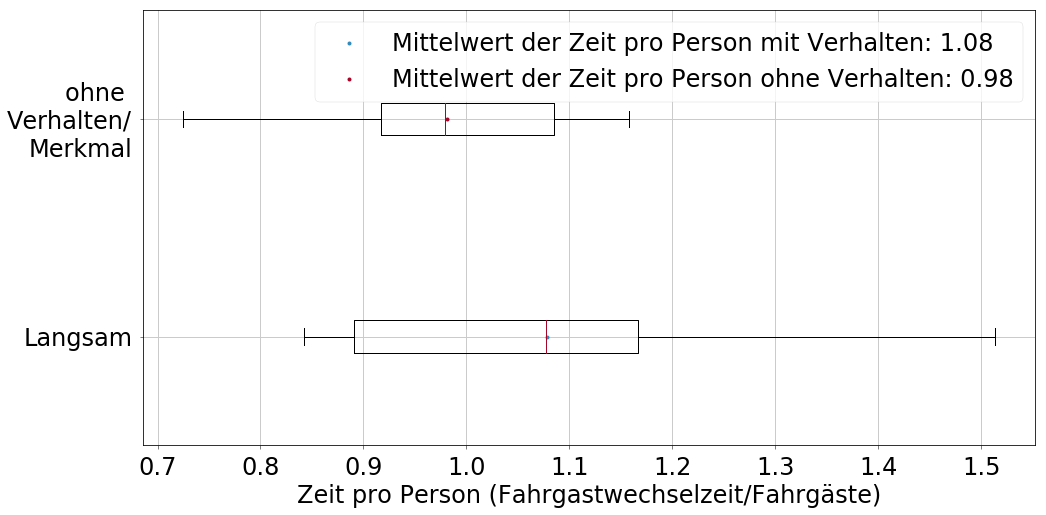
\includegraphics[width=0.8\textwidth]{pictures/data_evaluation/behavior/comp_Langsam.png}
	\caption{Box-Plot für den Vergleich der Zeiten pro Person für Personen die langsam sind und für Personen ohne das Merkmal "`langsam"'.}
	\label{fig:BoxPlotLangsam}
\end{figure}
Wie auf \figurename \ref{fig:BoxPlotLangsam} zu sehen ist hat sich die Fahrgastwechselzeit pro Personen durch langsame Personen im Fahrgastwechsel erhöht. Zu erkennen ist dies durch die Rechtsverschiebung des Box-Plots und dem erhöhten Mittelwert. Ob diese Erhöhung der Zeit signifikant ist, und das Merkmal damit in das Modell aufgenommen werden soll, wird durch den Vergleich von Quantilen entschieden. Zu diesem Zweck verglich ich den Median der Zeit pro Person, mit diesem Merkmal, mit dem oberen Quartil der Zeit pro Person, ohne das Merkmal. Dadurch wird gewährleistet, dass (weniger als) 25\% der Fahrgastwechselzeiten pro Person langsamer waren als das 50\% Quantil der Fahrgäste mit diesem Merkmal. Ist dies gegeben gehe ich davon aus, dass die Auswirkung des Merkmales auf die Zeit signifikant ist und dieses modelliert werden sollte.\\
Der Median der Zeit pro Person für die Fahrgastwechsel in denen "`langsame"' Personen vorkamen liegt bei 1.078 Sekunden. Das obere Quartil für Fahrgastwechsel ohne langsame Personen liegt jedoch bei 1.086 Sekunden. Auch wenn das Quartil der Daten ohne "`Langsame"' nur leicht den Median der Zeiten mit diesen überschreitet, scheint das Merkmal "`langsam"' keinen signifikanten Einfluss auf die gesamten Fahrgastwechselzeiten zu besitzen. Das Merkmal "`langsam"' einer Person wird somit nicht in das Modell mit aufgenommen.

Als nächstes untersuche ich die Auswirkung des Merkmals "`sperrig"'. Hierbei betrachtete ich die Fahrgastwechselzeiten von Videos, in denen zwischen 20 und 27 Personen gefilmt wurden. Auch hierbei ist auf dem Box-Plot, \figurename \ref{fig:BoxPlotSperrig}, zu erkennen das sich die Fahrgastwechselzeit pro Person durch das Merkmal erhöht hat. Während der Mittelwert der Zeiten ohne Sperrige noch bei 0.812 Sekunden lag, liegt er bei den Daten die Personen mit diesem Merkmal bei 0.871 Sekunden.
\begin{figure}[H]
	\centering
		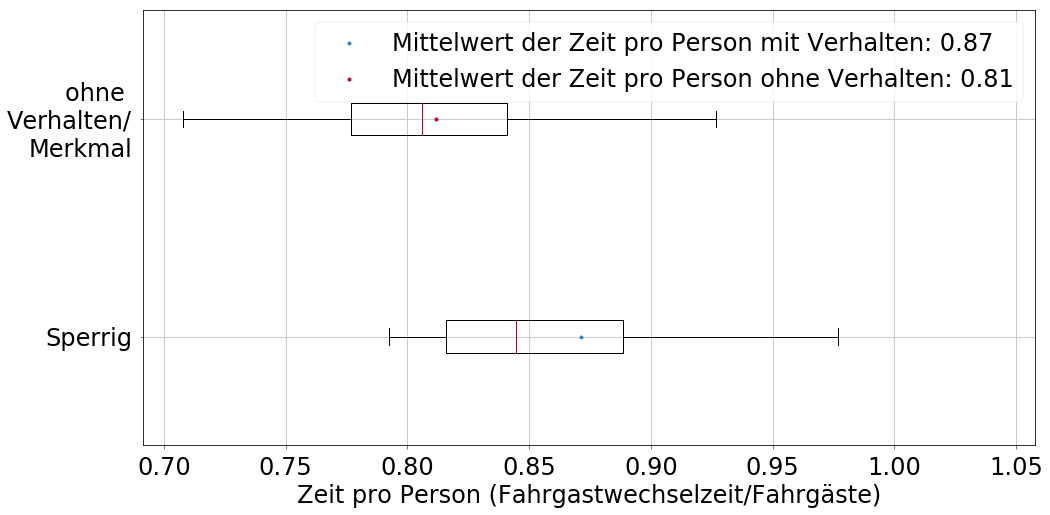
\includegraphics[width=0.8\textwidth]{pictures/data_evaluation/behavior/comp_Sperrig.png}
	\caption{Box-Plot für den Vergleich der Zeiten pro Person für Fahrgastwechsel in denen Personen sperrig sind mit Fahrgastwechsel ohne diese Personen.}
	\label{fig:BoxPlotSperrig}
\end{figure}
Bei diesem Merkmal liegt das obere Quartil der Zeit pro Person, für Personen ohne das Merkmal, bei 0.841 Sekunden, während der Median der Daten mit sperrigen Personen bei 0.844 Sekunden liegt. Da der Median für Personen mit dem Merkmal über dem oberen Quartil der Zeiten ohne dieses liegt, kann gesagt werden, dass der Unterschied signifikant ist. Zudem vermutete ich vor dem genaueren Betrachten, dass das Merkmal "`sperrig"' den Fahrgastwechsel verlangsamen könnte. Durch sperrige Personen kann es passieren, dass nicht mehr, wie im Normalfall, zwei Personen gleichzeitig durch die Tür gehen können, sondern nacheinander Aussteigen müssen, was zu einer Verlangsamung des Prozesses führen könnte. Da der zeitliche Einfluss des Merkmals erklärt werden kann und die Bedingung für die Quantile der Daten erfüllt ist, wird angenommen, dass das Merkmal "`sperrig"' signifikant ist und in das Modell aufgenommen werden sollte.

Als letztes Merkmal untersuche ich nun noch das Merkmal "`abgelenkt"'. Beim Vergleich handelt verwende ich die Fahrgastwechselzeiten für eine Anzahl von 13 bis 21 Personen. Auch für abgelenkte Personen hat sich die Fahrgastwechselzeit pro Person scheinbar erhöht. Es ist jedoch schon deutlich auf dem Bild, \figurename \ref{fig:BoxPlotAbgelenkt}, zu erkennen, dass das 75\%-Quantil der Zeiten für Personen ohne Abgelenkte nicht mehr unter dem Median der Zeiten für Fahrgastwechsel mit diesen liegt.
\begin{figure}[H]
	\centering
		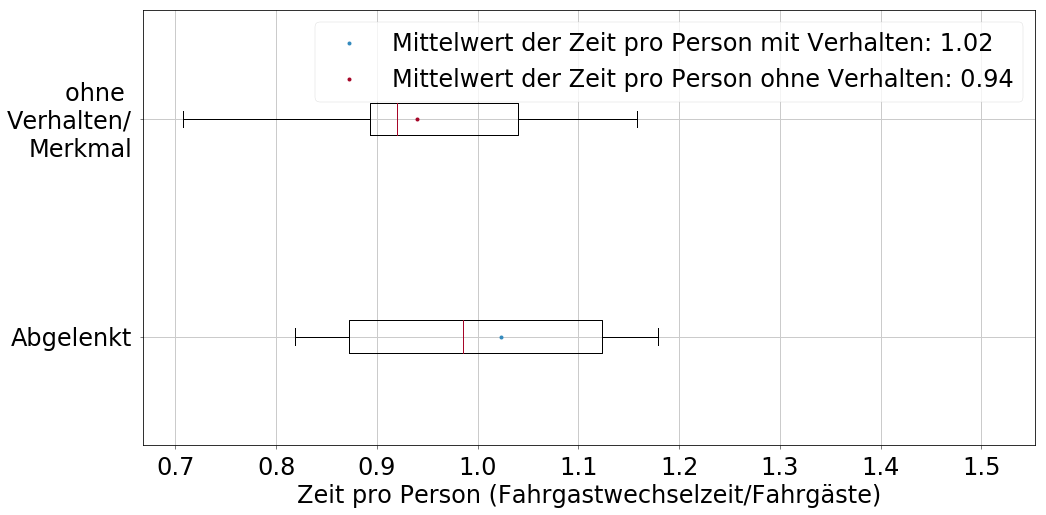
\includegraphics[width=0.8\textwidth]{pictures/data_evaluation/behavior/comp_Abgelenkt.png}
	\caption{Box-Plot für den Vergleich der Zeiten pro Person für Fahrgastwechsel in denen Personen vorkommen, die durch Gegenstände in ihrer Hand abgelenkt sind mit Fahrgastwechseln ohne abgelenkte Personen.}
	\label{fig:BoxPlotAbgelenkt}
\end{figure}
Die Signifikanz des Unterschieds ist somit deutlich geringer als vermutet. Dies ist wohl damit zu erklären, dass Personen, die durch Gegenstände in ihrer Hand vom Wechsel abgelenkt sind, sich nicht permanent mit diesem Gegenstand (\zB Handy oder Zeitung) beschäftigen. Sie sehen immer wieder auf, um zu wissen in welche Richtung sie gehen und Kollisionen sowie ein langsames Gehen zu vermeiden .

Abschließend zur Untersuchung der Merkmale, beantworte ich nun die Forschungsfrage \ref{item:Vehalten,Merkmale} "`Beeinflussen die Merkmale "`sperrig"', "`langsam"' und "`abgelenkt"' der Fahrgäste die Fahrgastwechselzeit? "'. Das Merkmal "`sperrig"' hat einen Einfluss auf die Fahrgastwechselzeit pro Person. Die Merkmale "`langsam"' und "`abgelenkt"' scheinen jedoch keinen signifikanten Einfluss auf die Zeiten des Fahrgastwechsels zu besitzen. Deshalb setze ich im Modell nur das Merkmal "`sperrig"' um. Die Merkmale "`abgelenkt"' und "`langsam"' berücksichtige ich für das Modell nicht. 

Als nächstes untersuche ich noch die Verhaltensweisen "`früher Einsteigen"' und "`im Weg Stehen"' auf ihren Einfluss auf die Zeit.\\
Bei der Verhaltensweise "`früher Einsteigen"' vermute ich, dass dieses Verhalten zu einer schnelleren Fahrgastwechselzeit pro Person führt. Diese wird nämlich, abgesehen von wenigen Ausnahmen, dann gezeigt, wenn Aussteigenden nur noch auf einer Seite der Tür in einer Reihe ausstiegen. Deshalb vermutete ich, dass die Fahrgastwechselzeit durch das frühzeitige Einsteigen sich im Gegensatz zum Warten verringert wird, oder zumindest gleichbleibt. Die Vermutung überprüfe ich durch den Vergleich der Fahrgastwechselzeiten von 12 bis 20 Personen. Auf dem Box-Plot, \figurename \ref{fig:BoxPlotFrueherEinsteigen}, ist jedoch zu sehen, dass sich die Zeit pro Person nicht verringert, sondern scheinbar sogar erhöht hat. Da diese Erhöhung jedoch nicht signifikant ist, erkennbar durch die Boxen, und ich die Veränderung so nicht erwartet habe, kann davon ausgegangen werden, dass diese Verhaltensweise keinen signifikanten zeitlichen Einfluss besitzt. Im Modell stelle ich sie jedoch trotzdem dar, um den Fahrgastwechsel besser simulieren zu können, ihr Einfluss auf die Zeit sollte bei Simulationen jedoch nicht beachtet werden.
\begin{figure}[H]
	\centering
		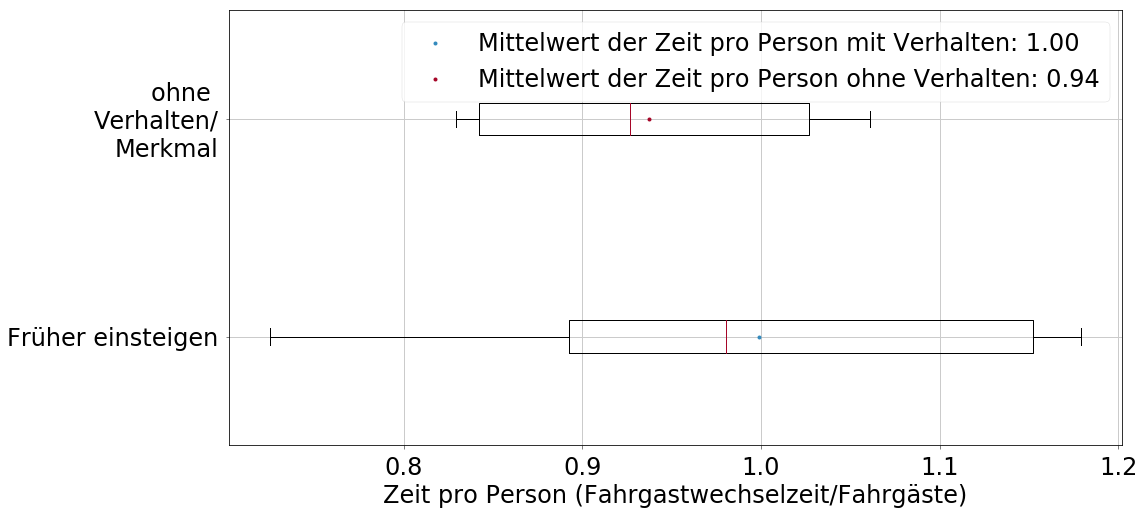
\includegraphics[width=0.8\textwidth]{pictures/data_evaluation/behavior/comp_Fruehereinsteigen.png}
	\caption{Box-Plot für den Vergleich der Zeiten pro Person für Fahrgastwechsel bei denen Personen vor Beendigung des Ausstiegsprozess Einsteigen mit, der Zeit pro Person für Fahrgastwechsel ohne Früher-Einsteiger.}
	\label{fig:BoxPlotFrueherEinsteigen}
\end{figure}
Bei der Verhaltensweise "`im Weg Stehen"' zeigt sich wie erwartet, auch eine Veränderung nach rechts, wenn die Fahrgastwechselzeiten für 19 bis 27 Personen verglichen werden. Diese Veränderung kann auf \figurename \ref{fig:BoxPlotImWeg} betrachtet werden.
\begin{figure}[H]
	\centering
		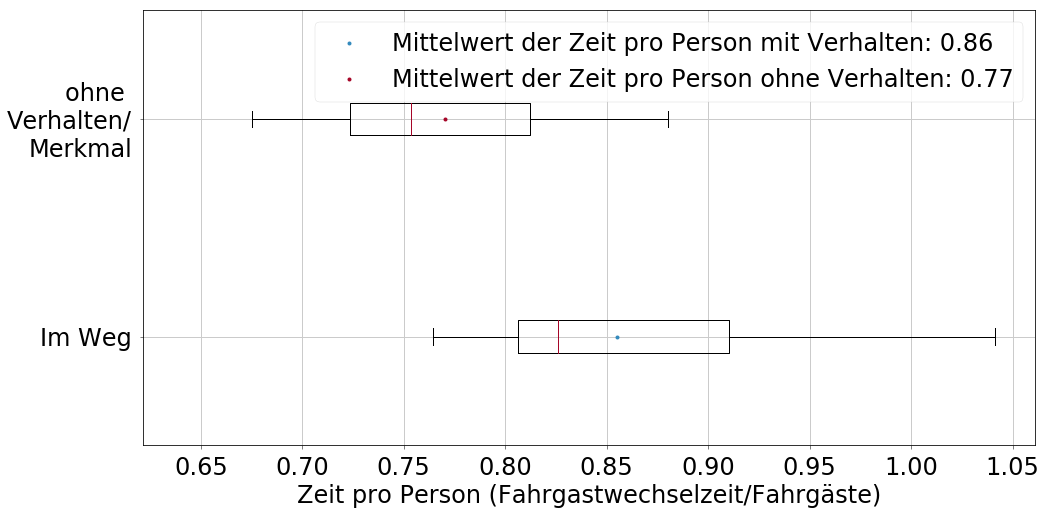
\includegraphics[width=0.8\textwidth]{pictures/data_evaluation/behavior/comp_ImWeg.png}
	\caption{Boxplot für den Vergleich der Zeiten pro Person für Personen die im Weg stehen und für andere Personen.}
	\label{fig:BoxPlotImWeg}
\end{figure}
Der Mittelwert für Fahrgastwechselzeiten pro Person mit im Weg stehenden Personen liegt mit 0.876 Sekunden über dem Wert der Zeit pro Person ohne dieses Verhalten der bei 0.806 Sekunden liegt. Zudem liegt auch das obere Quartil der Zeit mit 0.836 Sekunden pro Person unter dem Median der Fahrgastwechselzeit pro Person mit Videos bei denen Personen die "`im Weg Stehen"'. Dieser Median beträgt 0.841 Sekunden. Somit ist davon auszugehen, dass diese Verhaltensweise signifikant ist und wird deshalb in das Modell mit aufgenommen. Zudem könnte nach der Simulation gemessen werden, ob sich die Zeit der Fahrgastwechsel erhöht, wenn in einer Simulation Personen vorkamen, die im Weg standen. Der Einfluss könnte also zur Validierung des Modelles beitragen.

Auch nach der Auswertung der Verhaltensweise beantworte ich die zugehörige Forschungsfrage, \ref{item:Verhalten,Verhalten} "`Beeinflussen die Verhaltensweisen "`früher Einsteigen"' und "`Im Weg Stehen"' die Fahrgastwechselzeiten?"'. Die Verhaltensweise "`früher Einsteigen"' scheint keinen Einfluss auf die Zeit zu besitzen, während das Verhalten "`im Weg Stehen"' genau diesen zu besitzen scheint. Ich bilde jedoch beide Verhaltensweisen im Modell ab, da das Modell auf dem Verhalten der Fahrgäste und ihrem Entscheidungsprozess beruht. Deshalb ist deshalb wichtig die auffälligen Verhaltensweisen zu modellieren, um ein gutes Modell zu erhalten.

Nachdem ich den zeitlichen Einfluss der genannten Merkmale und Verhaltensweisen untersucht habe, überprüfe ich nun noch, ob es möglich ist einen Zusammenhang zwischen der Anzahl von Aussteigern und dem Auftreten von Platzmachern herzustellen.

Um den Zusammenhang, zwischen der Anzahl an Aussteigern und dem Vorkommen von Platzmachern, zu untersuchen führe ich eine logistische Regression durch. Die logistische Regression wird im Anhang in \ref{append:LogReg} noch einmal erklärt. Für den Zusammenhang in diesem Fall ist die Zielvariable das Vorkommen der Platzmacher und kodiert durch:
$$Platzmacher_i = 
	\begin{cases}
		1 & \text{falls ein Platzmacher in Fahrgastwechsel} \ i \ \text{vorkommt,} \\
		0 & \text{sonst.}
	\end{cases}$$
Um die logistische Regression zur Abschätzung des Auftretens von Platzmachern durchzuführen verwende ich das Logit-Modell:
\begin{equation}
P(Platzmacher=1) = \frac{\exp(\beta_0 + \beta_1 \cdot Anzahl \ Aussteiger)}{1+\exp(\beta_0 + \beta_1 \cdot Anzahl \ Aussteiger)}
\end{equation}
In der Bibliothek \texttt{statsmodels.discrete.discrete\_model} gibt es die Funktion \texttt{Logit}, mit der logistische Regressionen durchgeführt werden können. Diese Funktion wurde in \textsf{Jupyter Notebook} folgendermaßen aufgerufen:
\begin{lstlisting}[language=Python]
from statsmodels.discrete.discrete_model import Logit
from statsmodels.tools import add_constant

constant = add_constant(alight)
log_reg_spacemaker = Logit(cod_spacemaker, constant).fit()
\end{lstlisting}
Die Variable \texttt{alight} beschreibt die Anzahl der Aussteiger für die gefilmten Fahrgastwechsel. Die Methode \texttt{add\_constant} fügt an das \texttt{Array} der Anzahlen der Aussteiger eine Spalte mit Einsen ein. Wie ihr Name schon sagt, sorgt diese Methode dafür, dass auch eine Konstante (hier $\beta_0$) im Modell vorhanden ist. Die Variable \texttt{cod\_spacemaker} ist ein \texttt{Array}, dass die Kodierung für das Vorkommen von Platzmachern an einem Fahrgastwechsel enthält. Das Ergebnis der \texttt{fit} Methode ist ein \texttt{LogitResult} und enthält unter anderem die Schätzparameter und $p$-Werte von Hypothesentests.

Die Grafik mit der zurückgegebenen Schätzfunktion $$P(Platzmacher=1) = \frac{\exp(-2.96+0.09 \cdot Anzahl \ Aussteiger)}{1+\exp(-2.96+0.09 \cdot Anzahl \ Aussteiger)},$$
den Datenpunkten und dem Konfidenzintervall kann in \figurename \ref{fig:LogRegPM} betrachtet werden.
\begin{figure}[H]
	\centering
		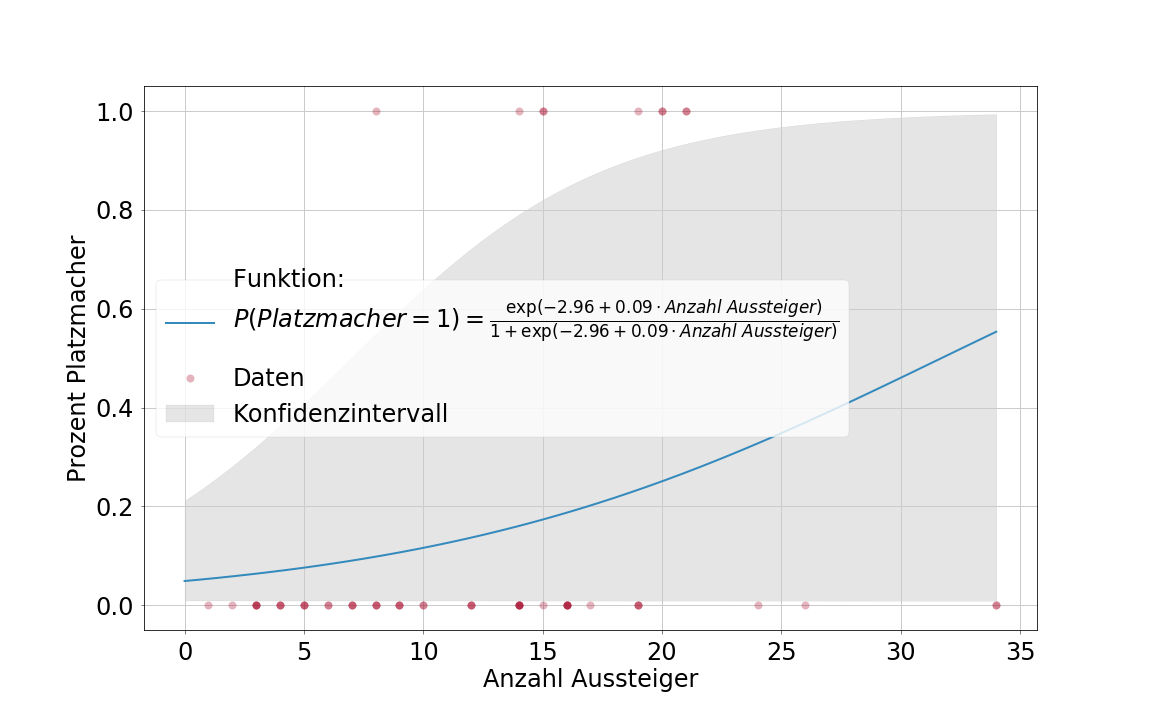
\includegraphics[width=0.8\textwidth]{pictures/data_evaluation/behavior/log_reg_spacemaker.png}
	\caption{Schätzfunktion der logistischen Regression mit der Zielvariable Platzmacher ($y$) und Kovariable Anzahl Aussteiger ($x$) mit Datenpunkten und Konfidenzintervall. Schätzfunktion: $P(y=1) = \frac{e^{-2.96+0.9 \cdot y}}{1 + e^{-2.96 + 0.9 \cdot y}}$}
	\label{fig:LogRegPM}
\end{figure}
Wie auf dem Bild zu erkennen sind die Konfidenzintervalle sehr groß und auch der $p$-Wert der t-Statistik für $\beta_1$ liegt mit $0.05$ über dem Signifikanzniveau von $0.01$. Mit meinen Daten kann also nicht modelliert werden, wann Platzmacher auftreten. Deshalb muss die Forschungsfrage \ref{item:Platzmacher} "`Gibt einen Zusammenhang zwischen der Anzahl der Aussteiger und dem Vorkommen von Platzmachern?"', mit, wohl eher nicht, beantwortet werden. \\
Es ist möglich, dass die Anzahl der Aussteiger einen gewissen Einfluss auf das Auftreten von Platzmachern hat. Mit der Anzahl der Aussteiger alleine kann jedoch nicht bestimmt werden, ob bei diesem Fahrgastwechsel ein Platzmacher auftreten wird. Ich schätze, dass der Zusammenhang weniger mit der Anzahl der Aussteiger zu tun hat, sondern eher damit, wie viele Personen sich im Wagon befinden in Kombination mit der Anzahl an Personen, die aussteigen wollen und der Position eines potenziellen Platzmacher. Eine weitere Untersuchung, die diese These überprüft, wäre mit Sicherheit interessant für das Modell.

Die Auswertungen der Verhaltensweisen und Merkmale sowie die logistische Regression des Zusammenhangs von Platzmachern und Aussteigern wurde in der Datei \textsl{Behavior.ipynb} durchgeführt die im Zusatzmaterial zu finden ist.

\section{Typen von Personen} \label{Typen}
In letzten Auswertungen beschäftige ich mich mit den Forschungsfragen \ref{item:Typen,Typen} "`Gibt es einen signifikanten Anteil an defensiven und aggressiven Personen?"' und \ref{item:Typen,Startzeiten} "`Liegen die Startzeiten der Aussteiger für die unterschiedlichen Typen in unterschiedlichen Intervallen?"'. Für die Untersuchung der Anteile von Typen werte ich die Tabelle der Typen, \tablename \ref{tab:Types} aus. Um die Forschungsfrage bezüglich der Startzeiten zu beantworten verwende ich dann die Tabelle der Startzeiten der Aussteiger \tablename \ref{tab:Startingtime}.

Im Folgenden werden die Anteile der Typen für die unterschiedlichen Prozesstypen (Einsteiger, Aussteiger und Platzmacher) in Kuchendiagrammen gezeigt. Für diese Aufteilung entscheide ich mich, da ich vermute, dass sich die Typen gegenseitig beeinflussen und durch die Art des Prozesses in der sich eine Person gerade befindet bedingt werden. Ich entschied mich dafür, dass ein Anteil signifikant ist, wenn er von mehr als 10 Prozent der Personen gezeigt wird.

Zunächst betrachte ich Anteile der Typen für Einsteiger. 
\begin{figure}[H]
	\centering
		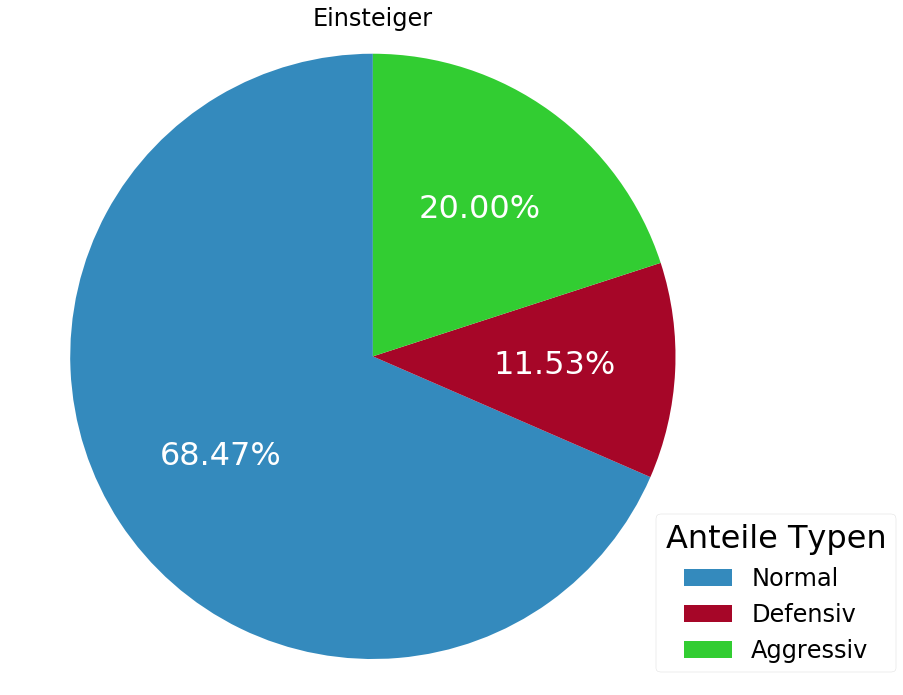
\includegraphics[width=0.6\textwidth]{pictures/data_evaluation/types/proportions_Einsteiger.png}
	\caption{Kuchendiagramm der Anteile der Typen aggressiv, defensiv und normal für den Prozesstypen Einsteiger (siehe \ref{Tabelle der Typen}).}
	\label{fig:AnteileTypenEinsteiger}
\end{figure}
Wie in \figurename \ref{fig:AnteileTypenEinsteiger} zu sehen ist, beobachtete ich am meisten normale Einsteiger, was an dem Anteil von \ca 68 \% zu erkennen ist. Mit einem Anteil von 20\% für aggressive und \ca 12\% für defensive Typen scheinen diese Typen jedoch auch signifikant zu sein. Es ist also davon auszugehen, dass ihre Modellierung zu einem besseren Modell führen würde. Die Forschungsfrage \ref{item:Typen,Typen} kann also zumindest für Einsteigende so beantwortet werden, dass ihr Anteil signifikant ist. 

In \figurename \ref{fig:AnteileTypenAussteiger} können die Anteile der Typen für Aussteiger betrachtet werden. 
\begin{figure}[H]
	\centering
		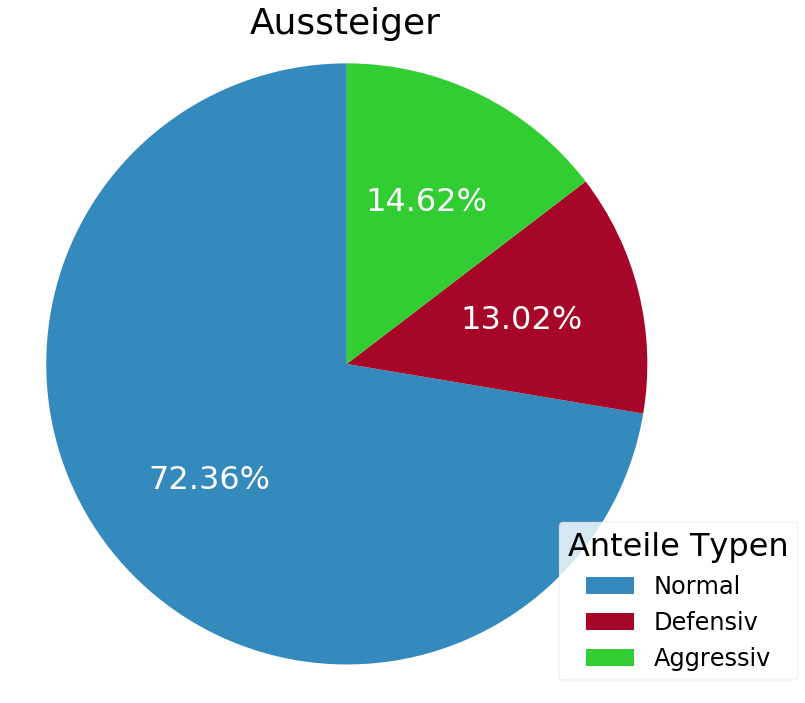
\includegraphics[width=0.6\textwidth]{pictures/data_evaluation/types/proportions_Aussteiger.png}
	\caption{Kuchendiagramm der Typen aggressiv, defensiv und normal für den Prozesstypen Aussteiger (siehe \ref{Tabelle der Typen}).}
	\label{fig:AnteileTypenAussteiger}
\end{figure}
In dem Kuchendiagramm ist zu erkennen, dass der größte Anteil an beobachteten Typen wieder der normale Typ ist. Diese Typen besitzen einen Anteil von \ca 72 \%. Jedoch gibt es auch einen signifikanten Anteil an defensiven und aggressiven Typen, wobei defensive einen Anteil von 13 \% und aggressive einen Anteil von \ca 15 \% ausmachen. Für Aussteiger ist die Frage \ref{item:Typen,Typen} also auch mit ja zu beantworten. Da es hier signifikante Anteile für die Typen defensiv und aggressiv gibt, wäre es gut auch die Aussteiger im Modell in aggressive, defensive und normale Typen zu unterteilen.

Als nächstes werte ich nun noch die Anteile der Platzmacher aus.
\begin{figure}[H]
	\centering
		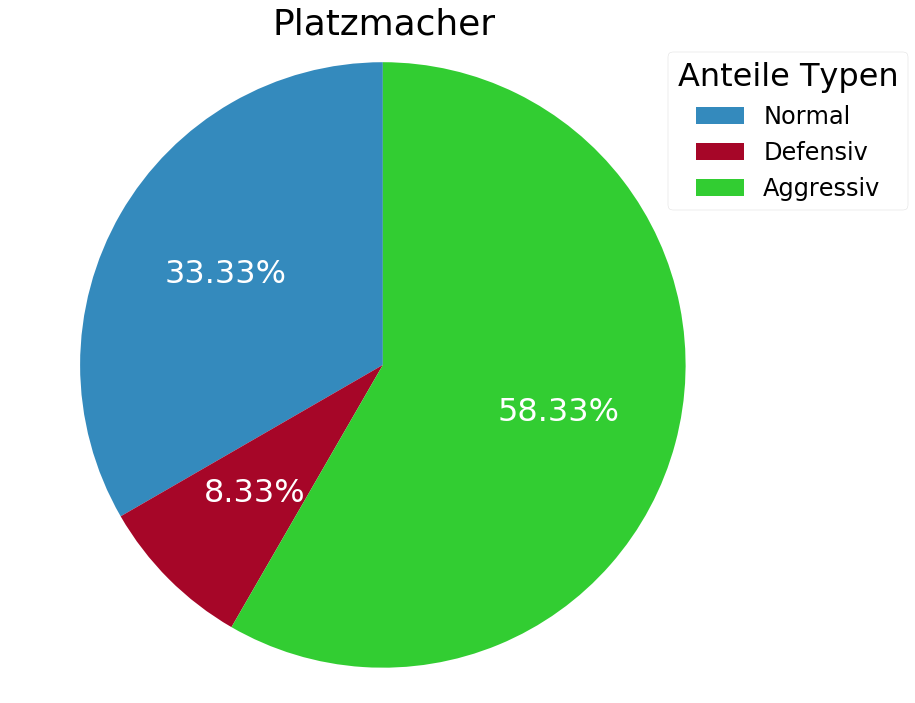
\includegraphics[width=0.7\textwidth]{pictures/data_evaluation/types/proportions_Platzmacher.png}
	\caption{Kuchendiagramm der Typen aggressiv, defensiv und normal für den Prozesstypen Platzmacher (siehe \ref{Tabelle der Typen}).}
	\label{fig:AnteileTypenPlatzmacher}
\end{figure}
In \figurename \ref{fig:AnteileTypenPlatzmacher} ist nun zuletzt das Kuchendiagramm der Anteile von Typen der Platzmacher zu sehen. Bei den Platzmachern überwiegen, im Gegensatz zu den anderen Prozesstypen, die aggressiven Typen mit über 50\% (53.85\%). Der Anteil der normalen Typen macht mit \ca 38\%  auch einen großen Anteil aus. Es gibt jedoch auch einen Anteil an defensiven Platzmacher. Mit 7.69\% scheinen diese jedoch nicht signifikant zu sein. Da der defensive Typ für Aussteiger und Einsteiger jedoch in das Modell mit aufgenommen werden soll, soll dieser auch für Platzmacher definiert werden, um das Modell konsistent zu halten. Es ist jedoch auch anzumerken, dass der Anteil von 7.69\% wahrscheinlich nur durch die geringe Anzahl an aufgenommenen Platzmachern zustande gekommen ist. Im Material wurde nur ein einziger defensiver Platzmacher gesehen, da ich jedoch nur sehr wenige Platzmacher beobachtet habe, ist nicht festzustellen, ob der Anteil sich verringern würde, wenn mehr Platzmacher beobachtet werden. Da die Platzmacher sowohl ein- als auch aussteigen, wird die Forschungsfrage auch für diesen Prozesstypen mit Ja beantwortet. 

Im Modell wird der Entscheidungsprozess der Personen dargestellt, hierbei passe ich die Ein- und Aussteiger sowie Platzmacher zudem für defensive, aggressive und normale an, da sich der Entscheidungsprozess für diese Typen unterscheidet. Dies kann am Beispiel der ersten Person, die aus dem Wagon aussteigt, erkannt werden. Während aggressive schon kurz nach der Türöffnung aussteigen, warten defensive bis diese komplett geöffnet ist und normale Personen bis die Tür etwas weiter geöffnet ist. Es ist jedoch schwierig in einer Simulation zu beschreiben, wie weit eine Tür geöffnet ist. Deshalb untersuchte ich, ob für die Typen aggressiv, defensiv und normal unterschiedliche Intervalle für die Startzeiten gefunden werden können. Mit den Intervallen wird dann modelliert, wann Aussteiger mit dem Aussteigen beginnen. Diese Untersuchung führe ich im nächsten Abschnitt, Abschnitt \ref{Startzeiten} durch.

Die Kuchendiagramme der Anteile von Typen für die unterschiedlichen Prozesstypen wurden in der Datei \textsl{TypesOfPeople.ipynb} mit \texttt{Python} erstellt.

\subsection{Startzeiten der Aussteiger für die Typen} \label{Startzeiten}
Nachdem ich im Vorangegangen erklärt habe, warum es interessant ist Aussteiger in unterschiedlichen Typen einzuteilen um modellieren zu können wann diese mit dem aussteigen beginnen, beantworte ich nun die aufgekommene Frage: "`Liegen die Startzeiten der Aussteiger für die unterschiedlichen Typen in unterschiedlichen Intervallen?"'\\
Zu diesem Zweck trug ich in der Tabelle der Startzeiten, \tablename \ref{tab:Startingtime}, die Zeiten aus den Videos ein, die verstreicht bevor die erste Person aus dem Zug aussteigt. Hier gab ich zudem in einer weiteren Spalte der Tabelle an, welchem Typ der erste Aussteiger in diesem Video zuzuordnen ist. 

Mit den Daten aus der Tabelle erstellte ich Box-Plots für die Startzeiten der Typen, die in \figurename \ref{fig:BoxPlotStartingTime} betrachtet werden können.
\begin{figure}[H]
	\centering
		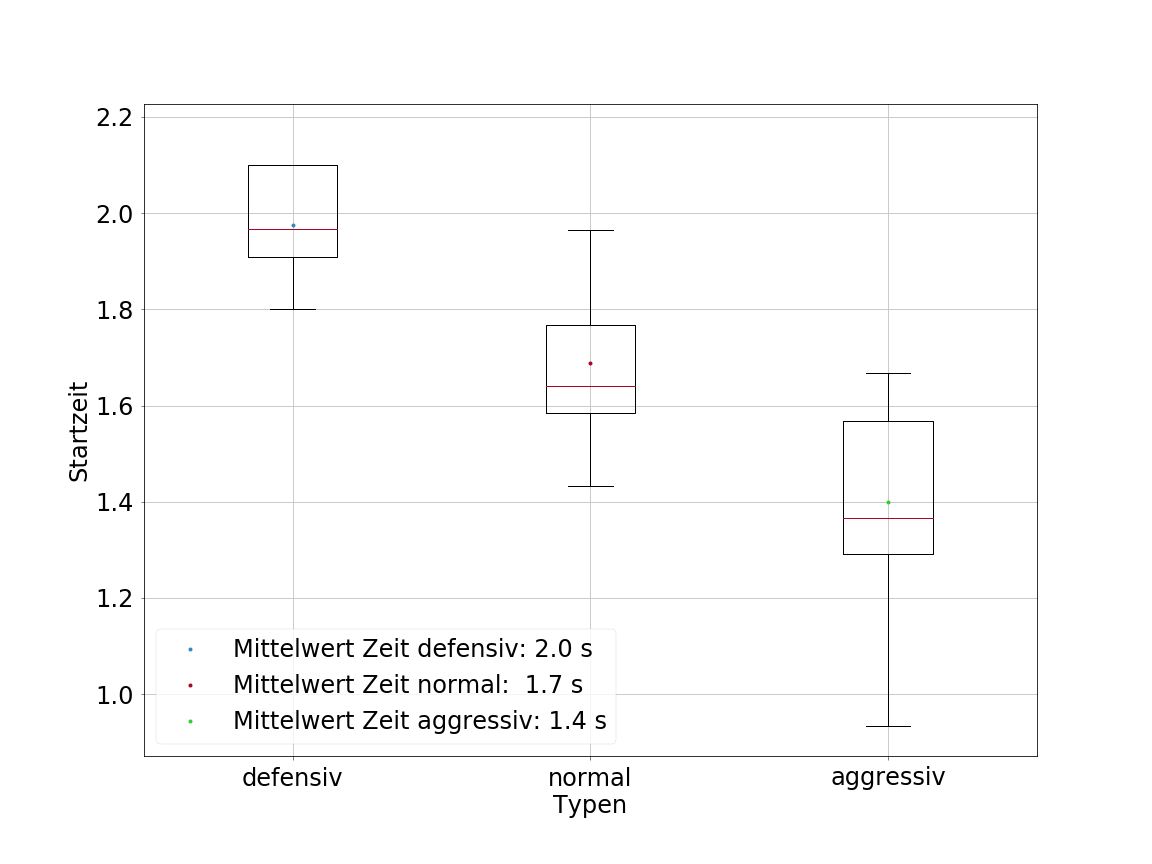
\includegraphics[width=1.0\textwidth]{pictures/data_evaluation/types/starting_time/starting_times.png}
	\caption{Box-Plots der Startzeiten für die unterschiedlichen Typen aggressiv, defensiv und normal von Aussteigern.}
	\label{fig:BoxPlotStartingTime}
\end{figure}
Auf diesem Plot ist zu erkennen, dass sich die Startzeiten der Aussteiger für die unterschiedlichen Typen defensiv, aggressiv und normale unterscheidet, wie ich bei der Beobachtung vermutet habe. Während die defensiven mit 2.0 Sekunden im Mittel am längsten warten, ergeben die Mittelwerte für normale und aggressive Typen das diese im Mittel 1.7 \bzw 1.4 Sekunden warten, bevor sie mit dem Aussteigen anfangen. Für die Startzeit soll jedoch kein fester Wert verwendet werden, sondern jeweils ein Zeitraum für defensive, aggressive und normale gewählt werden. Hierfür untersuchte ich die Histogramme der Startzeiten für die Typen. Da jedoch nur sehr wenige Daten vorhanden sind, konnten diese nicht auf ihre Verteilung untersucht werden. Deshalb entschied ich, dass der Zeitraum durch die Quartile festgelegt wird. Für die untere Schranke des Startzeitraums wählte ich jeweils das 25\%-Quantil, für die obere das 75\%-Quantil, der Startzeiten für den entsprechenden Typ. \\ 
Damit ergibt sich für die Intervalle: \\
Startzeiten Intervall für den Typ "`normal"' $= [1.6, 1.8]$ Sekunden. \\
Startzeiten Intervall für den Typ "`aggressiv"' $= [1.3, 1.6]$ Sekunden. \\
Startzeiten Intervall für den Typ "`defensiv"'$= [1.9, 2.1]$ Sekunden. 

Es kann also gesagt werden, dass ein Zeitraum für die Startzeiten für verschiedene Typen von Aussteigern festgelegt werden konnte. Damit ist auch die Forschungsfrage \ref{item:Typen,Startzeiten} beantwortet worden. Die definierten Intervalle sollen später im Modell für den Entscheidungsprozess der Aussteiger verwendet werden.

\chapter{Modell} \label{Modell}
In diesem Kapitel erstelle ich ein Modell für den Fahrgastwechsel, und erkläre wie durch dieses die Ergebnisse der Datenauswertung umgesetzt werden. Zunächst beschreibe ich jedoch das bisher verwendete Modell von accu:rate. Daraufhin erstelle ich das Fahrgastwechsel-Modell. Dabei beschreibe ich auch das kognitive Heuristik Modell, auf dem mein Fahrgastwechsel-Modell aufbaut. Nachdem ich das Modell, die Umsetzung der Auswertung und die Grenzen des Modells erklärt habe, beschreibe ich dann den Algorithmus für dieses und die benötigten Parameter.
\section{Modell von accu:rate} \label{Accurate Modell}
Schon in früheren Projekten hat, accu:rate, Personenströme an U-Bahnstationen in München simuliert. Bis jetzt warten, in der Modellierung von accu:rate, die Personen rechts und links der Türen in Wartezonen. Diese Modellierung wird dabei vom Nutzer ertellt und ist nicht in der crowd:it Software implementiert. Die Wartezeit wird bei diesem Modell vor der Simulation festgelegt. Die Wartezeit wird bestimmt, indem berechnet wird wie lange die sich im Zug befindeten Personen, benötigen, um auszusteigen. Nach Ablauf der Wartezeit beginnen die wartenden Personen den Zug zu betreten. Da, wie in \ref{Stand der Technik} erwähnt, das Modell von accu:rate jedoch nicht auf empirischen Beobachtungen beruht, erstelle ich im Nachfolgenden ein Fahrgastwechsel-Modell, das ich auf Grundlage der angestellten Auswertungen der Daten erstellt habe. Das Modell erweitert crowd:it um kognitive Entscheidungsprozesse, sodass zukünftig nicht dem Nutzer das Modellieren von Verhalten überlassen werden muss, sondern die Software selbst das Verhalten abbilden kann. Diese Entscheidungsprozesse verwenden dabei Heuristiken des kognitiven Heuristik Modells nach \cite{Seitz.2016}. 
\section{Fahrgastwechsel-Modell} \label{Fahrgastwechsel-Modell}
Das Fahrgastwechsel-Modell modelliert den Ein- und Ausstiegsprozess sowie den Platzmachprozess. Für diese Prozesse werden unterschiedliche Heuristiken verwendet. In jeder dieser Heuristiken gibt es zudem Unterschiede für die unterschiedlichen Typen: aggressiv, defensiv und normal. \\
Das Fahrgastwechsel-Modell habe ich mit Hilfe des kognitiven Heuristik Modell umgesetzt, welches von Michael Seitz in seiner Dissertation vorgestellt wird (\cite{Seitz.2016}). Dieses Modell ist in der Software crowd:it zwar implementiert worden, wurde jedoch noch nicht für alle Fälle empirisch untersucht und getestet. Deshalb wird dieser Teil im Moment nicht verwendet. In der Dissertation von Michael Seitz überprüft dieser jedoch sein Modell mit zwei Szenarien durch Simulationen. Mit den Ergebnissen dieser Simulationen wird sein Modell durch den Vergleich mit den Ergebnissen aus kontrollierten Experimenten validiert. Dabei wurden zum einen die Ergebnisse für das Gehen durch einen Engpass (eng.: "`bottleneck"'), zum anderen die Ergebnisse eines bidirektionalen Flusses durch einen Korridor verglichen (\cite{Seitz.2016}). Mit eben diesen Szenarien kann der Fahrgastwechsel beschrieben werden. Wenn die Personen beim Fahrgastwechsel gleichzeitig ein- und aussteigen, kann dies als bidirektionaler Fluss durch einen Korridor beschrieben werden. Steigen Personen nur ein oder aus, so bewegen sich die Personen durch die Tür die als Engpass gesehen werden kann. In seiner Arbeit kommt \cite{Seitz.2016} zu dem Ergebnis, dass sein Ansatz für eine Fußgängersimulation mit diesen Szenarien geeignet ist. Nachdem genau die Szenarien untersucht wurden, mit denen ein Fahrgastwechsel beschrieben werden kann, nehme ich an, dass ich das Fahrgastwechsel-Modell auf diesem aufbauen kann. Das kognitive Heuristik Modell nach \cite{Seitz.2016} erkläre ich in Abschnitt \ref{CHM}.

Im dem von mir erstellten Fahrgastwechsel-Modell modelliere ich das Verhalten der Personen auf dem Bahnsteig und im Zug nicht, sondern nur der Fahrgastwechsel an sich. Soll in Zukunft auch das Verhalten im Inneren des Zuges und am Bahnsteig simuliert werden, kann mein Modell mit anderen bereits existierenden kombiniert werden. Für das Verhalten Einsteiger und Platzmacher nach dem Einsteigen kann das Modell der Sitzplatzwahl verwendet werden, dass Jakob Schöttl in seiner Masterarbeit an der Hochschule München erstellt hat (\cite{Schottl.2016}). Nachdem Aussteiger den Zug verlassen haben, kann zudem das bereits von crowd:it verwendete "`Optimal Steps"'-Modell für den weiteren Pfad der Aussteiger verwendet werden.
\subsection{Das kognitive Heuristik Modell} \label{CHM}
\cite{Seitz.2016} stellt in seiner Dissertation vier Heuristiken vor: die "`Step or wait"'-Heuristik, die "`Tangential evasion"'-Heuristik, die "`Sideways evasion"'-Heuristik und die "`Follower"'-Heuristik. Ich verwende die englischen Bezeichnungen im Folgenden weiterhin, um Verwirrungen durch undeutliche Übersetzungen zu verhindern. Bei der "`Step or wait"'-Heuristik gehen Personen einen Schritt in die Richtung des Ziels, wenn ihr Pfad frei ist und verbleiben in ihrer derzeitigen Position, falls nicht. Die "`Tangential evasion"'-Heuristik bringt Personen dazu, tangential auszuweichen, wenn ihr Pfad blockiert wird. Die "`Sideways evasion"'-Heuristik bringt Agenten zusätzlich dazu, seitlich auszuweichen, falls die "`tangential evasion"' nicht möglich ist. Die "`Follower"'-Heuristik lässt Agenten einen anderen Agenten suchen dem gefolgt werden kann, der in die gleiche Richtung geht, wenn der direkte Pfad zum Ziel blockiert wird (\cite{Seitz.2016}). Die Algorithmen für diese Heuristiken werden in \ref{Algorithmus} beschrieben. \\
Bei der Simulation mit der kognitiven Heuristik wird den Agenten zu Beginn ein Ziel zugeordnet. Wenn sie ihr Ziel erreicht haben, gehen sie entweder zu ihrem nächsten Ziel oder werden aus dem Szenario entfernt, wenn dieses Ziel ihr finales Ziel ist (\cite{Seitz.2016}). Für den Fahrgastwechsel bedeutet das, dass für Aussteiger die Ziele auf dem Bahnsteig hinter dem Wartebereich der Einsteiger liegen.
Die Skizze mit eingezeichnetem Ziel-Bereich für Aussteiger kann in \figurename \ref{fig:SkizzeAussteiger} betrachtet werden. Der Zielbereich der Aussteiger ist in dieser Abbildung durch rote Rechtecke gekennzeichnet.
\begin{figure}[H]
	\centering
		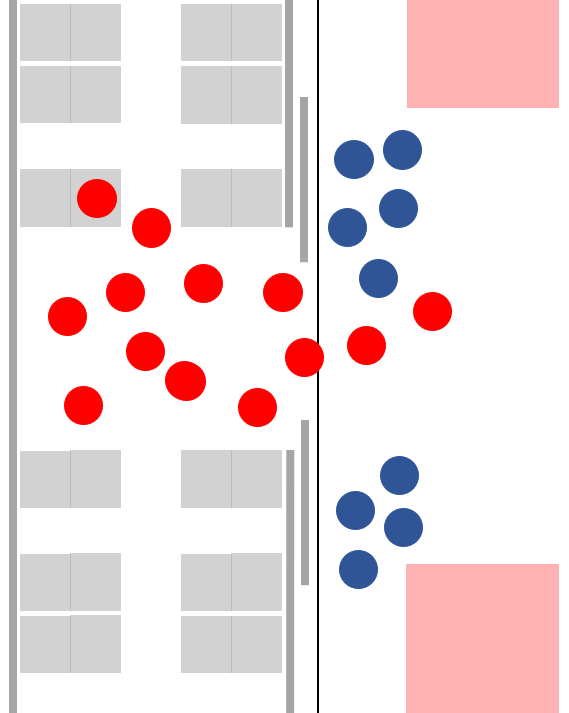
\includegraphics[angle=270, width=0.5\textwidth]{pictures/model/kognitive_heuristic_model/alight_sketch.png}
	\caption{Skizze zur Darstellung der Zielbereiche von Aussteigern aus der Vogelperspektive: U-Bahn "`Wände"' dargestellt durch graue Linien, Sitzplätze der U-Bahn durch graue Vierecke, Bahnsteigkante durch schwarze Linie, Aussteiger durch rote Kreise und Einsteiger durch blaue Kreise. Der Zielbereich ist mit einem roten Rechteck gekennzeichnet.}
	\label{fig:SkizzeAussteiger}
\end{figure}
Einsteiger und Platzmacher besitzen als Zwischenziel den Wartebereich. Einsteiger beginnen den Fahrgastwechsel am Bahnsteig in einigem Abstand vom Gleis. Von diesem Startpunkt bewegen sie sich zum Zwischenziel, einen Wartebereich rechts oder links der Türen. Ihr endgültiges Ziel liegt im Wagon kurz hinter den Türen.
Die Skizze für die Bereiche der Einsteiger kann in \figurename \ref{fig:SkizzeEinsteiger} genauer angesehen werden.
\begin{figure}[H]
	\centering
		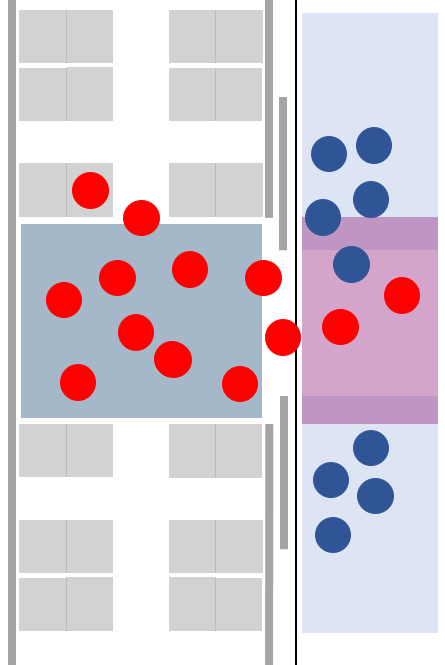
\includegraphics[angle=270, width=0.5\textwidth]{pictures/model/kognitive_heuristic_model/boarding_sketch.png}
	\caption{Skizze zur Darstellung der Zwischenzielbereiche und Zielbereiche von Einsteigen aus der Vogelperspektive: Die Zwischenzielbereiche sind in hellblau und lila, der Zielbereich in dunkelblau eingezeichnet.}
	\label{fig:SkizzeEinsteiger}
\end{figure} 
Der Zwischenzielbereich der Einsteiger, ist in dieser Abbildung, \figurename \ref{fig:SkizzeEinsteiger} in hellblau eingezeichnet. Zu diesem Zwischenziel kann auch der in lila dargestellte Bereich, der "`Im Weg"'-Bereich werden, wenn eine Person aufgrund der Heuristik im Weg steht. Der Zielbereich der Einsteiger ist in dunkelblau dargestellt.

Platzmacher starten im Wagon und gehen zunächst auch in die Wartebereiche neben den Türen, danach ist ihr Ziel dasselbe wie bei den Einsteigern, siehe \figurename \ref{fig:SkizzePlatzmacher}.
\begin{figure}[H]
	\centering
		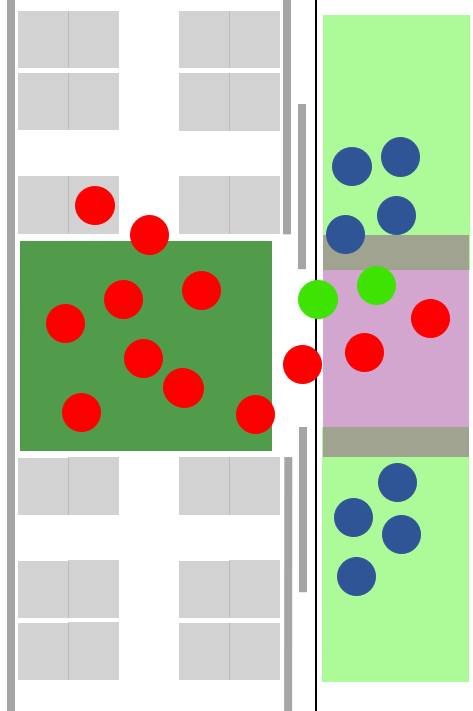
\includegraphics[angle=270, width=0.5\textwidth]{pictures/model/kognitive_heuristic_model/spacemaker_sketch.png}
	\caption{Skizze zur Darstellung der Zwischenzielbereiche und Zielbereiche von Platzmachern aus der Vogelperspektive: Platzmacher werden durch grüne Kreise dargestellt. Zwischenzielbereiche sind in hellgrün und lila, der Zielbereich in dunkelgrün eingezeichnet.}
	\label{fig:SkizzePlatzmacher}
\end{figure}
Der Zwischenzielbereich der Platzmacher, ist in hellgrün eingezeichnet. Zu diesem Zwischenziel kann auch, der in lila dargestellte Bereich, der "`Im Weg"'-Bereich werden, wenn eine Person aufgrund der Heuristik im Weg steht. Der Zielbereich der Platzmacher ist in dunkelgrün dargestellt.
\subsection{Grenzen des Modells}
In meinem Fahrgastwechsel-Modell, wird immer nur eine Tür des Zuges modelliert. Wie sich Personen für eine Tür oder einen Wagon entscheiden, wird somit außer Acht gelassen. Auch ein Umentscheiden einer Person an einer anderen Tür auszusteigen als zunächst geplant wird in diesem Modell nicht bearbeitet, ein Verhalten das auf ein paar der Videos aufgenommen wurde.\\
In meinem Modell weichen Personen, die "`im Weg stehen"' nicht aus, wenn sich andere Personen auf sie zubewegen oder sich an ihnen vorbei drängen. Dieses Verhalten wurde auf Videos von Personen gezeigt, die den Weg anderer versperren. Dieses Verhalten wird jedoch nicht in das Modell mit aufgenommen. \\
In meinem Modell steigen alle im Zug vorhandenen Personen aus dem Zug aus, um auf den Bahnsteig zu gelangen oder Platz zu machen. Personen, die im Zug bleiben und möglicherweise einen Einfluss auf die Fahrgastwechselzeit besitzen, werden nicht modelliert. Zudem gibt es in meinem Modell keine Personen am Bahnsteig, die nicht an der Tür einsteigen wollen. \\
Eine weitere Grenze meines Modells betrifft die Platzmacher. Platzmacher reagieren auf das Bedürfnis von Personen hinter ihnen im Wagon. Sie treten auf, wenn Aussteiger hinter ihnen aus dem Wagon drängen und der Platzmacher keine Möglichkeit hat diesen innerhalb des Wagons auszuweichen. In meinem Modell werden Platzmacher jedoch einfach zu einer übergebenen Anzahl eingesetzt, da kein Zusammenhang zwischen der Anzahl der Aussteiger und dem Auftreten von Platzmachern hergestellt werden konnte und eine Information über die Anzahl der Personen im Wagon nicht erhoben wurde.
\subsection{Umsetzung der Auswertungen}
Bevor ich die Algorithmen für den Fahrgastwechsel und die darin enthaltenen Algorithmen für die Heuristiken erkläre, beschreibe ich in den nächsten Abschnitten, wie die Auswertungen im Modell dargestellt werden sollen.
\subsubsection{Fahrgastwechselzeit}
Die Auswertungen der Fahrgastwechselzeit \ref{Zeiten} werden nicht direkt im Modell verwendet. Sie dienen nur der Validierung und Kalibrierung des Modells. Mit dem Vergleich der aufgenommenen Wechselzeiten mit den Wechselzeiten einer Simulation könnten die Parameter des Algorithmus angepasst werden. Zudem kann mit ihnen nach Simulationen mit diesem Modell überprüft werden ob diese reale Ergebnisse liefern, und das Modell somit Valide ist.
\subsubsection{Gruppen}
Wie im Abschnitt \ref{Gruppen} bereits erklärt, kann die Auswertung für Gruppen nicht direkt in die Software von crowd:it eingesetzt werden. Hier muss zunächst die Übergabe der Gruppen verändert werden. Deshalb werden Gruppen in diesem Modell nicht umgesetzt.
\subsubsection{Verhaltensweisen und Merkmale}
In der Auswertung der Verhaltensweisen und Merkmale, Abschnitt \ref{Verhalten}, kam ich zu dem Schluss, dass das Merkmal "`sperrig"' sowie die Verhaltensweisen "`früher Einsteigen"' und "`im Weg Stehen"' im Modell dargestellt werden sollen. 

Um das Merkmal "`sperrig"' umzusetzen, soll die Schulterbreite der Personen, die in crowd:it angegeben werden kann, verwendet werden. Aus den Daten ergibt sich für den Mittelwert des Anteils von Sperrigen Personen pro Tür ein Anteil von 4.05 \%. Damit ich dieses Merkmal umsetzten kann wird bei 4 \% der Population des Fahrgastwechsel die Schulterbreite auf das 1.5 Fache der ursprünglichen Schulterbreite erhöht. Durch diese Erhöhung werden Personen sperrig und es ist nicht mehr immer möglich zu zweit durch die Tür zu gehen.

Die Verhaltensweisen "`früher Einsteigen"' und "`im Weg Stehen"' setze ich mit den Heuristiken der Prozesstypen um. Bei den Heuristiken der normalen und aggressiven Einsteiger wird abgefragt, wie viel Platz in der Tür vorhanden ist. Ab einer bestimmten Breite Platz in der Tür (genauer erklärt in \ref{EM}), beginnen diese Einsteiger mit dem Einsteigen. So steigen Normale und Aggressive früher ein, wenn Platz in der Tür ist, auch wenn Personen noch aussteigen. Da für Platzmacher die "`Einsteigeprozess"'-Heuristik verwendet wird, tritt durch mein Modell auch bei diesem Prozesstypen das Verhalten "`früher Einsteigen"' auf.\\
Die Verhaltensweise "`im Weg Stehen"' wird in meinem Modell von aggressiven Einsteigern und Platzmachern gezeigt. Hier wird die Verhaltensweise für Platzmacher umgesetzt, indem sie die "`Einsteigeprozess"'-Heuristik verwenden, wenn sie aus dem Wagon ausgestiegen sind. Durch die "`aggressive Platzsuche"'-Heuristik wird die Verhaltensweise "`Im Weg Stehen"' umgesetzt, die in \ref{Verhalten} als signifikant für den Prozess eingestuft wurde. Es wird dazu angenommen, dass diese Verhaltensweise nur auftritt, wenn aggressive Personen vorne oder neben der vordersten Person im Wartebereich keinen Platz finden.

Eine weitere Verhaltensweise die ich in \ref{Verhalten} untersucht habe, ist das Platz machen. Dieses Verhalten wird durch die Modellierung der Prozesstypen Platzmacher umgesetzt. Bei der Auswertung kam ich zu Ergebnis, dass das Vorkommen von Platzmachern nicht durch die Anzahl der Aussteiger abgeschätzt werden kann. Deshalb wird die Anzahl der Platzmacher manuell übergeben, dabei können die, in \ref{Beschreibung der Daten} angegebenen Anteile als Referenz verwendet werden.
\subsubsection{Typen von Personen}
In der Auswertung \ref{Typen} kam ich zu dem Fazit, dass die unterschiedlichen Typen aggressiv, defensiv und normal dargestellt werden sollen, da sie einen signifikanten Anteil besitzen. Im Modell modelliere ich also die in \ref{Tabelle der Typen} angegebenen Verhaltensweisen durch die, die unterschiedlichen Typen auf den von mir erstellten Videos erkannt wurden. Die Verhaltensweise für normale Personen, durch die Tür gehen, wenn genügend Platz in der Tür ist, wurde durch die "`Einsteigeprozess"'-Heuristik umgesetzt. Hierbei wird der Platz in der Tür berechnet, ist dieser größer oder gleich dem 1.2 Fachen der normalen Person, so beginnt diese mit dem Einsteigen. Für Aussteiger wurde dies durch die ebenfalls ausgewerteten Startzeiten umgesetzt. Bei Aussteigern ist der Platz in der Tür dadurch bestimmt, wie weit die Tür geöffnet ist. Nachdem es schwierig ist, in einer Simulation darzustellen, wie weit eine Tür geöffnet ist wurden für Aussteiger die Startzeiten verwendet. Hierbei wird aus dem Intervall der Startzeiten für normale Aussteiger zufällig eine Startzeit für die Person ausgewählt. Es wird dabei angenommen, dass die Startzeiten normal verteilt sind. Auch für aggressive Personen wurde das Merkmal, dass sie durch die Tür gehen, wenn etwas Platz in der Tür ist, durch die Abfrage des Platzes in der Tür und der zufälligen Wahl einer Startzeit aus dem Intervall für aggressive umgesetzt. Das Merkmal für defensive, die nur durch die Tür gehen, wenn keine andere Person in der Tür ist, wird umgesetzt, indem die Heuristik von Michael Seitz angepasst wird. Im Modell von Michael Seitz gehen Personen einen Schritt nicht, wenn dieser zu einer Kollision führt. In meinem Modell nehmen defensive Personen den Schritt auch dann nicht, wenn sie durch diesen den Türbereich betreten würden und sich in diesem gerade eine Person befindet. Sind sie bereits im Türbereich gehen sie jedoch normal durch die Tür. Das sie normal durch die Tür gehen, sobald sie den Türbereich betreten haben, verhindert, dass eine Person stehen bleibt, wenn eine Person nach ihr den Türbereich betritt. Ein weiteres Merkmal von aggressiven Typen ist, dass sie sich vor andere Personen drängen und ihnen dabei sogar in den Weg laufen. Deshalb wird für diese Typen die "`Follower"'-Heuristik angepasst. In der "`Follower"'-Heuristik, die von normalen und defensiven verwendet wird, sucht die Person zunächst eine Person der sie folgen kann, wenn auf dem Weg zum Ziel ein Hindernis liegt. Erst wenn kein Leader gefunden wird, versuchen diese Personen, ihre nächste Position durch die "`Sideways evasion"'-Heuristik zu finden. Aggressive Typen verwenden in meinem Modell jedoch zunächst die "`Sideways evasion"'-Heuristik. Wird hierdurch keine neue mögliche Position gefunden, versuchen auch aggressive Typen einer Person zu folgen, um voran zu kommen. Dadurch überholen sie Personen vor sich. Um darzustellen, dass Aggressive auch in den Weg laufen, gehen diese im Algorithmus immer zuerst ihren Schritt, daraufhin versuchen Normale und dann Defensive sich voran zubewegen. Durch die "`Platzsuche"'-Heuristik wird dargestellt, dass normale Platzmacher sich so weit vorne wie möglich in den Wartebereich stellen, Defensive sich hinter die letzte Person im Wartebereich stellten und Aggressive immer vor die erste Person stellen. Die Heuristik wird in der Heuristik des Einsteigeprozesses verwendet, welcher wiederum von Platzmachern nach dem Aussteigen verwenden wird. Bei diesen Heuristiken suchen Normale nach dem nächsten freien Platz nahe an der Tür und defensive stellen sich hinter die letzte Person im Wartebereich. Aggressive hingegen wollen sich immer ganz vorne in den Wartebereich stellen. Ist vor oder neben der ersten Person kein Platz, so Positionieren sie sich im "`Im Weg"'-Bereich. Auch die ausgewerteten Startzeiten werden im Modell verwendet, wie für Normale und Aggressive bereits erwähnt. Auch für Defensive wird die Startzeit zufällig, diesmal aus dem Intervall der Startzeiten für Defensive, gewählt.
\section{Algorithmus} \label{Algorithmus}
Zur Erklärung der Heuristiken wird zunächst das Prozessdiagramm beschrieben und daraufhin ein Pseudocode angegeben, mit dem dieses umgesetzt werden kann. Dabei wird immer ein Schritt des Agenten dargestellt. In der Simulation werden die Heuristiken also so oft wiederholt, bis die Person den Zielbereich erreicht hat. Zunächst wird der Einsteigeprozess, anschließend der Ausstiegsprozess und zum Schluss der Platzmachprozess erläutert. Bei der Erklärung der "`Einsteigeprozess"'-Heuristik, werden zudem die Algorithmen der kognitiven Heuristiken nach \cite{Seitz.2016} beschrieben.
\subsection{Einsteiger-Heuristik} \label{EM}
Das Prozessdiagramm für die Heuristik des Einsteigeprozess, ist in \figurename \ref{fig:EH} dargestellt. 
\begin{figure}[H]
	\centering
		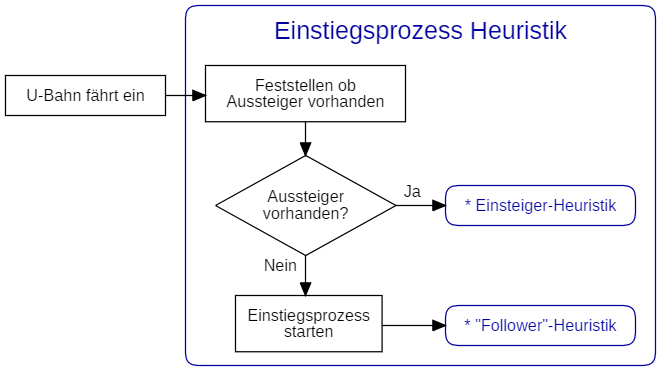
\includegraphics[width=0.9\textwidth]{pictures/model/algorithm/boarding/boarding_process.png}
	\caption{Prozessdiagramm der Einsteiger: "`Einsteigeprozess"'-Heuristik.}
	\label{fig:EH}
\end{figure}
Will eine Person an einer Tür einsteigen, so wird zunächst überprüft ob an dieser Tür Aussteiger vorhanden sind. Ist dies nicht der Fall, so können die Einsteiger durch Verwendung der "`Follower"'-Heuristik, bei aggressiven Einsteigern durch der "`aggressive Follower"'-Heuristik, sofort mit dem Einsteigen in den Zug beginnen. Gibt es jedoch Personen, die durch diese Tür auf den Bahnsteig gelangen wollen, so wird für die unterschiedlichen Typen die jeweilige "`Einsteiger"'-Heuristik verwendet. Der Algorithmus des Einsteigeprozesses, könnte im Code wie folgt umgesetzt werden:

\begin{algorithm} [H]
	\caption{"`Einsteigeprozess"'-Heuristik}
	\SetKwInOut{Output}{Output}
	\SetKwProg{BoardingHeuristic}{BoardingHeuristic}{}{}
	
	\Output{$pos_p$ nächste gewünschte (eng.: "`preferred"') Position}
	\BoardingHeuristic{} {
		Überprüfen ob Aussteiger vorhanden \\
		Typ der Person ist $T$\\
		\If{Aussteiger vorhanden} {
			\uIf{$T$ ist defensiv} { 
				$pos_p = $ \textbf{DefensiveBoardingHeuristic}
			}\uElseIf {$T$ ist normal} {
				$pos_p = $ \textbf{NormalBoardingHeuristic} 	
			} \Else {
				$pos_p = $ \textbf{AggressiveBoardingHeuristic}
			}
		} \Else {
			Ziel des Agenten auf den Bereich im Inneren des Wagons setzten \\
			\If{$T$ ist aggressiv} {
				$pos_p = $ \textbf{AggressiveFollowerHeuristic}		
			} \Else {
				$pos_p = $ \textbf{FollowerHeuristic}		
			}
		}
		\Return $pos_p$
	}
\end{algorithm}

Gibt es keine Aussteiger, so muss die "`Einsteige"'-Heuristik für den entsprechenden Typ nicht verwendet werden, da diese auf dem Vorkommen von Aussteigern beruhen. Die Einsteiger können sofort mit der entsprechenden "`Follower"'-Heuristik mit dem Einsteigen beginnen. Dazu wird das Ziel des Agenten auf den Bereich im Inneren des Zuges gesetzt. Das Ziel des Agenten wird bei Einsteigern erst im Algorithmus festgelegt, da sich das Ziel im Laufe des Algorithmus auf ein Ziel im Wartebereich ändern kann, wenn die Person nicht direkt einsteigen kann. Dieser Fall wird in den unterschiedlichen "`Einsteige"'-Heuristiken abgeprüft. Bevor die Heuristiken für normale, defensive und aggressive Einsteiger beschrieben werden, wird zunächst der Algorithmus der "`Follower"'-Heuristik beschrieben. Dieser Algorithmus, wird auch im Ausstiegs- und Platzmachprozess verwendet.

\cite{Seitz.2016} definiert die "`Follower"'-Heuristik, wie in \figurename \ref{fig:followerHeuristik} dargestellt.
\begin{figure}[H]
	\centering
		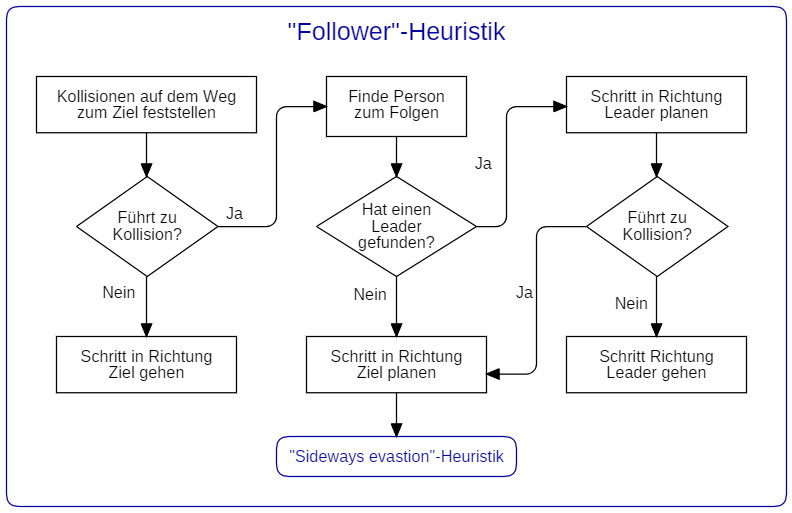
\includegraphics[width=1.0\textwidth]{pictures/model/algorithm/heuristics/follower_heuristic.png}
	\caption{Prozessdiagramm der "`Follower"'-Heuristik nach \cite{Seitz.2016}.}
	\label{fig:followerHeuristik}
\end{figure}
Wird bei der "`Follower"'-Heuristik eine Kollision auf dem Weg zum Ziel erkannt, so versucht der Agent die nächste Person zu finden, die in dieselbe Richtung geht. Ist ein solcher Leader gefunden, geht der Agent seinen nächsten Schritt in Richtung dieses Leaders. Wenn kein Leader gefunden wird oder der Schritt in Richtung Leader zu einer Kollision führen würde, so wird die "`Sideways evasion"'-Heuristik verwendet (\cite{Seitz.2016}). Der Pseudocode der "`Follower"'-Heuristik mit angepasster Abfrage für defensive kann in Algorithmus \ref{alg:Follower} betrachtet werden.
\clearpage
\begin{algorithm} [H]
	\caption{"`Follower"'-Heuristik}
	\label{alg:Follower}
	\SetKwInOut{Output}{Output}
	\SetKwProg{FollowerHeuristic}{FollowerHeuristic}{}{}
	
	\Output{$pos_p$ nächste gewünschte (eng.: "`preferred"') Position}
	\FollowerHeuristic{} {
		Zielrichtung bestimmen \\
		Direkter Pfad zum Ziel berechnen \\
		Pfad auf Kollisionen prüfen \\
		$T_d$ ist \True wenn Typ der Person $T$ defensiv ist, \False falls nicht \\
		\If{Weg führt zu Kollision} {
			Finde Person $L$ zum folgen \\
			\If{$L$ gefunden} { 
				Schritt $pos_L$ in Richtung Leader $L$ berechnen \\
				\If{$pos_L$ führt zu Kollision \Or ($T_d$ \Andnot \textbf{StepPossible}$(pos_{current}, pos_{L})$)} {
					$pos_p$ = \textbf{SidewaysEvasionHeuristic}
				} \Else {
					Schritt in Richtung Leader gehen: $pos_p = pos_L$ 
				}
			} \Else {
				$pos_p$ = \textbf{SidewaysEvasionHeuristic}	
			}
		} \Else {
			nächste Position $pos_{Ziel}$ in Richtung Ziel berechnen \\
			Schritt in Richtung Ziel gehen: $pos_p = pos_{Ziel}$		
		}
		\Return $pos_p$
	}
\end{algorithm}

Liegt auf dem Weg ein Hindernis, wird versucht eine Person der gefolgt werden kann, ein Leader, zu finden. Wird kein Leader gefunden, wird der Algorithmus \ref{alg:SidewaysEvasion} der "`Sideways Evasion"'-Heuristik verwendet, um den nächsten Schritt zu finden. Für die Abfrage bei defensiven Typen wird dabei der Algorithmus \ref{alg:StepPossible} verwendet, um zu überprüfen ob die defensive Person einen Schritt gehen kann. 
\clearpage
\begin{algorithm} [H]
	\caption{Test für defensive Agenten}
	\label{alg:StepPossible}
 	\SetKwInOut{Input}{Input}
 	\SetKwInOut{Output}{Output}
	\SetKwProg{StepPossible}{StepPossible}{}{}
	
	\Input{$pos_{current}$ aktuelle Position des Agenten \newline
	$pos_{next}$ nächste gewünschte Position des Agenten}
	\Output{Boolean Wert, der angibt ob die nächste Position für defensive Agenten möglich ist: \True, wenn möglich }
	\StepPossible{$(pos_{current}$, $pos_{next})$} {
		\If{$pos_{current} \notin$ Türbereich \AND $pos_{next} \in$ Türbereich \AND andere Person im Türbereich} {
		\Return \False
		}\Else {
		\Return \True
		}
	}
\end{algorithm} 

Um herauszufinden ob der nächste Schritt für die Person möglich ist, wird überprüft, ob die Person sich derzeit außerhalb des Türbereich befindet, mit dem nächsten Schritt in den Türbereich eintreten würde und ob sich im Moment eine andere Person im Türbereich befindet. Sind diese Bedingungen gegeben, gibt die Funktion den Boolean Wert "`False"' zurück, da ein Schritt in diesem Fall, in diese Richtung nicht möglich ist. Für die Überprüfung wird der Funktion die aktuelle Position und die zu überprüfende Position übergeben.

Neben dem \textbf{StepPossible} Algorithmus wird in der "`Follower"'-Heuristik auch der Algorithmus \ref{alg:SidewaysEvasion} \textbf{SidewaysEvasionHeuristic} verwendet. Die "`Sideways evasion"'-Heuristik wird in \figurename \ref{fig:sidewayHeuristik} erläutert.
\begin{figure}[H]
	\centering
		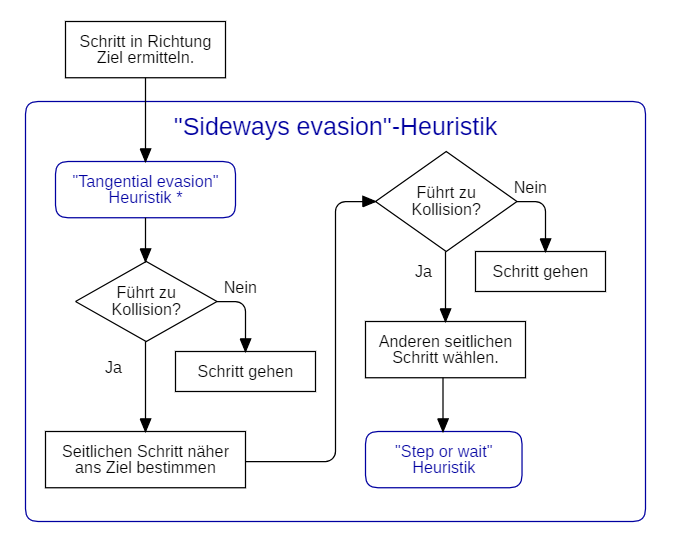
\includegraphics[width=0.9\textwidth]{pictures/model/algorithm/heuristics/sideways_evasion_heuristic.png}
	\caption{Prozessdiagramm der "`Sideways Evasion"'-Heuristik nach \cite{Seitz.2016}.}
	\label{fig:sidewayHeuristik}
\end{figure} 
Bei der "`Sideways evasion"'-Heuristik versuchen die Agenten zunächst die "`Tangential evasion"'-Heuristik zu verwenden, um zum Ziel zu gelangen. Dabei ist zu beachtet, dass die "`Step or wait"'-Heuristik die in  der "`Tangential evasion"'-Heuristik verwendet wird hier nicht angewandt wird. Gelingt das tangentiale Ausweichen nicht, wird versucht seitlich auszuweichen. Die "`Step or wait"'-Heuristik wird von den Agenten erst dann eingesetzt, wenn weder tangentiales noch seitliches Ausweichen möglich ist (\cite{Seitz.2016}). Der Algorithmus für die "`Sideways evasion"'-Heuristik mit meiner Anpassung für defensive Typen ist in Algorithmus \ref{alg:SidewaysEvasion} dargestellt.
\clearpage
\begin{algorithm} [H]
	\caption{"`Sideways evasion"'-Heuristik}
	\label{alg:SidewaysEvasion}
	\SetKwInOut{Output}{Output}
	\SetKwProg{SidewaysEvasionHeuristic}{SidewaysEvasionHeuristic}{}{}
	
	\Output{$pos_p$ nächste gewünschte (eng.: "`preferred"') Position}
	\SidewaysEvasionHeuristic{} {
		$pos_t =$ \textbf{TangentialEvasionHeurisic} \\
		$T_d$ ist \True wenn Typ der Person $T$ defensiv ist, \False falls nicht \\
		\If{zurückgegebene Position $pos_t$ ist $pos_{current}$} {
			speichern des Bereichs des Hindernisses oder Agenten $K$ \\
			berechnen beider seitlichen Umgehungsschritte $pos_c$ und $pos_d$ in Relation zu $K$ \\
			Position $pos_c$ hat die kleinerer Distanz zum Ziel \\
			\If{$pos_c$ führt zu Kollision \Or ($T_d$ \Andnot \textbf{StepPossible}$(pos_{current}, pos_{c})$} {
				\If{$pos_d$ führt zu Kollision \Or ($T_d$ \Andnot \textbf{StepPossible}$(pos_{current}, pos_{d})$} {
					In aktueller Position verbleiben $pos_p = pos_{current}$
				} \Else {
						zweiten seitlichen Schritt in Richtung Ziel gehen $pos_p = pos_d$
				}
			} \Else {
				ersten seitlichen Schritt in Richtung Ziel gehen $pos_p = pos_c$
			}
		} \Else {
			Schritt aus \textbf{TangentialEvasionHeuristic} gehen $pos_p = pos_{t}$		
		}
		\Return $pos_p$
	}
\end{algorithm}

Im \textbf{SidewaysEvasionHeuristic} Algorithmus wird zunächst der \textbf{TangentialEvasionHeuristic} Algorithmus durchgeführt. Gibt dieser Algorithmus als nächste erwünschte Position die jetzige Position des Agenten zurück, war ein direkter Schritt zum Ziel nicht möglich, und auch die Umgehungsschritte konnten nicht gewählt werden. Ist dies der Fall wird versucht seitlich auszuweichen.
Die "`Tangential evasion"'-Heuristik kann in \ref{fig:tangentialHeuristik} betrachtet werden.
\begin{figure}[H]
	\centering
		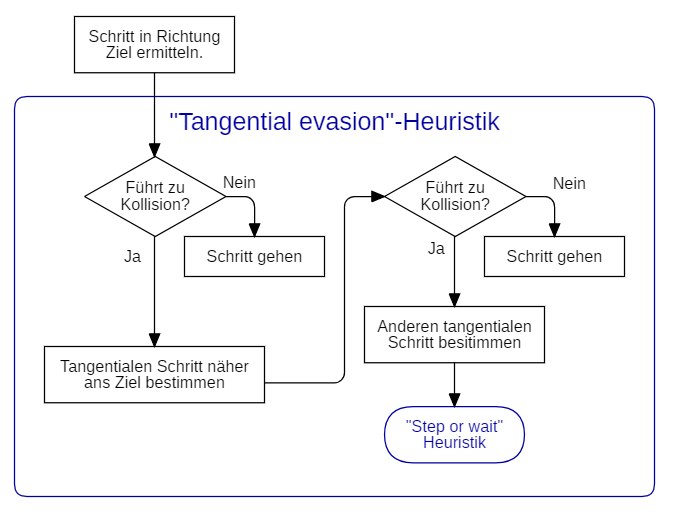
\includegraphics[width=0.9\textwidth]{pictures/model/algorithm/heuristics/tangential_evasion_heuristic.png}
	\caption{Prozessdiagramm der "`Tangential evasion"'-Heuristik nach \cite{Seitz.2016}.}
	\label{fig:tangentialHeuristik}
\end{figure} 
Die "`Tangential evasion"'-Heuristik lässt Agenten versuchen Kollisionen tangential auszuweichen. Wenn das tangentiale Ausweichen nicht möglich ist, so wird die "`Step or wait"'-Heuristik verwendet, was bedeutet, dass der Agent in seiner aktuellen Position verbleibt (\cite{Seitz.2016}). Der zugehörige Algorithmus, wird in Algorithmus \ref{alg:TangentialEvasion}, dargestellt.
\clearpage
\begin{algorithm} [H]
	\caption{"`Tangential evasion"'-Heuristik}
	\label{alg:TangentialEvasion}
	\SetKwInOut{Output}{Output}
	\SetKwProg{TangentialEvasionHeuristic}{TangentialEvasionHeuristic}{}{}
	
	\Output{$pos_p$ nächste gewünschte (eng.: "`preferred"') Position}
	\TangentialEvasionHeuristic{} {
		Zielrichtung bestimmen \\
		nächste Position $pos_{Ziel}$ in Richtung Ziel berechnen \\
		$T_d$ ist \True wenn Typ der Person $T$ defensiv ist, \False falls nicht \\
		\If{$pos_{Ziel}$ führt zu Kollision \Or ($T_d$ \Andnot \textbf{StepPossible}$(pos_{current}, pos_{Ziel})$)} {
			speichern des Bereichs des Hindernisses oder Agenten in $K$ \\
			berechnen der tangentialen Umgehungschritte $pos_a$ und $pos_b$ in Relation zu $K$  \\
			Position $pos_a$ ist die Position mit geringerer Distanz zum Ziel \\
			\If{$pos_a$ führt zu Kollision \Or ($T_d$ \Andnot \textbf{StepPossible}$(pos_{current}, pos_{a})$)} {
				\If{$pos_b$ führt zu Kollision \Or ($T_d$ \Andnot \textbf{StepPossible}$(pos_{current}, pos_{b})$)} {
					In aktueller Position verbleiben $pos_p = pos_{current}$
				} \Else {
					zweiten tangentialen Schritt in Richtung Ziel gehen $pos_p = pos_b$
				}
			} \Else {
				ersten tangentialen Schritt in Richtung Ziel gehen $pos_p = pos_a$			
			}
		} \Else {
			Schritt in Richtung Ziel gehen: $pos_p = pos_{Ziel}$		
		}
		\Return $pos_p$
	}
\end{algorithm}
 
Neben den vorgestellten Heuristiken mit der Anpassung für defensive Agenten, definiere ich zudem noch die "`aggressive Follower"'-Heuristik. Diese soll für aggressive Typen eingesetzt werden, da ich davon ausgehe, dass diese Agenten zunächst versuchen die "`Sideways evasion"'-Heuristik zu verwenden, bevor sie einer Person folgen.

\begin{figure}[H]
	\centering
		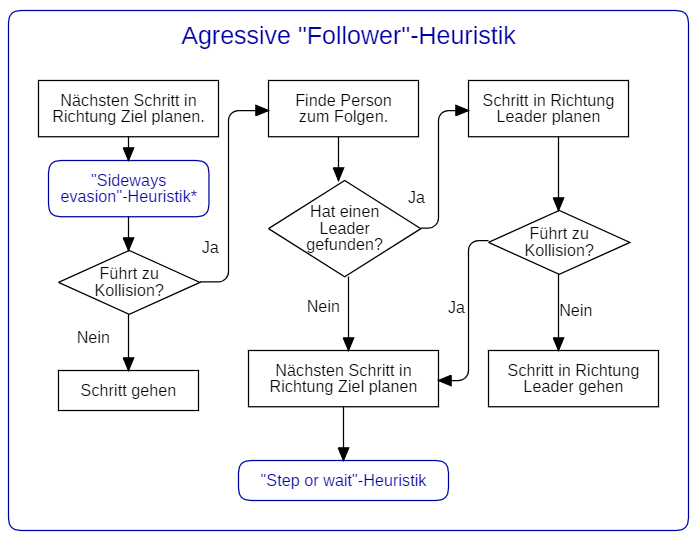
\includegraphics[width=1.0\textwidth]{pictures/model/algorithm/heuristics/aggressive_follower_heuristic.png}
	\caption{Prozessdiagramm der "`aggressiven Follower"'-Heuristik.}
	\label{fig:AFH}
\end{figure}
Bei der "`aggressiven Follower"'-Heuristik versucht der Agent seitlich und tangential auszuweichen, wenn der Weg zum Ziel versperrt ist. Sind auch die Ausweichmöglichkeiten versperrt, so wird versucht der nächsten Person in die gleiche Richtung zu folgen. Wenn jedoch kein Leader gefunden werden kann, oder ein Schritt in die Richtung von diesem zu einer Kollision führen würde, bleibt die Person stehen, sie verwendet die "`Step or wait"'-Heuristik. Der Algorithmus der "`aggressiven Follower"'-Heuristik ist in Algorithmus \ref{alg:aggressiveFollower} eingefügt.
\clearpage
\begin{algorithm} [H]
	\caption{"`aggressive Follower"'-Heuristik}
	\label{alg:aggressiveFollower}
	\SetKwInOut{Output}{Output}
	\SetKwProg{AggressiveFollowerHeuristic}{AggressiveFollowerHeuristic}{}{}
	
	\Output{$pos_p$ nächste gewünschte (eng.: "`preferred"') Position}
	\AggressiveFollowerHeuristic{} {
		$pos_s$ = \textbf{SidewaysEvasionHeuristic}\\
		\If{zurückgegebene Position $pos_s$ ist jetzige Position $pos_{current}$} {
			Finde Person $L$ zum folgen \\
			\If{$L$ gefunden} { 
				Schritt $pos_L$ in Richtung Leader berechnen \\
				\If{$pos_L$ führt zu Kollision} {
					In aktueller Position verbleiben $pos_p = pos_{current}$ 
				} \Else {
					Schritt in Richtung Leader gehen $pos_p = pos_L$
				}
			} \Else {
				In aktueller Position verbleiben $pos_p = pos_{current}$ 	
			}
		} \Else {
			Schritt aus \textbf{SidewaysEvasionHeuristic} gehen: $pos_p = pos_{s}$		
		}
		\Return $pos_p$
	}
\end{algorithm}

Gibt der Algorithmus \textbf{SidewaysEvasionHeuristic} eine neue Position zurück, so wird diese in der \textbf{AggressiveFollwerHeuristic} zurückgegeben. Ist das Ergebnis jedoch die jetzige Position, ein Schritt also nicht möglich, wird versucht einer anderen Person zu folgen.
Nachdem die "`Follower"'-Heuristiken und die Heuristiken die in diesen verwendet werden beschrieben wurden, werden nun die "`Einsteige"'-Heuristiken für Normale, Defensive und Aggressive beschrieben.

\subsubsection{Normaler Einsteiger} 
Für normale Einsteiger wird die "`normaler Einsteiger"'-Heuristik verwendet, welche in \figurename \ref{fig:NEH} gezeigt wird.
\begin{figure}[H]
	\centering
		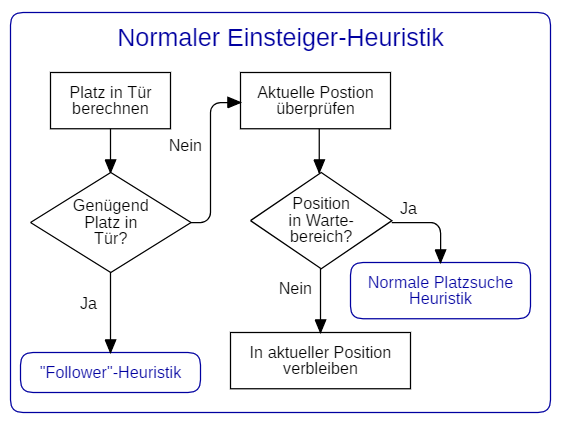
\includegraphics[width=0.8\textwidth]{pictures/model/algorithm/boarding/normal_boarding/normal_boarding_heuristic.png}
	\caption{Prozessdiagramm "`normaler Einsteiger"'-Heuristik.}
	\label{fig:NEH}
\end{figure}
Zunächst wird bei der "`normalen Einsteiger"'-Heuristik berechnet wie viel Platz im Türbereich ist. Ist genügend Platz in der Tür, beschrieben in \ref{Tabelle der Typen}, so beginnt der normale Einsteiger mit dem Einsteigen, was durch die "`Follower"'-Heuristik geschieht. Ist nicht genügend Platz wird überprüft, ob sich der Einsteiger bereits in einem Wartebereich befindet. Ist ein Agent bereits in einem Wartebereich, so verbleibt er in seiner aktuellen Position, er wartet, bis er einsteigen kann. Ist der Agent noch nicht im Wartebereich, so wird die "`normale Platzsuche"'-Heuristik verwendet, die im Anschluss erklärt wird. Zunächst wird jedoch der Algorithmus \ref{alg:NormalBoarding} \textbf{NormalBoardingHeuristic} erklärt. 
\clearpage

\begin{algorithm} [H]
	\caption{"`Normaler Einsteiger"'-Heuristik}
	\label{alg:NormalBoarding}
	\SetKwInOut{Output}{Output}
	\SetKwProg{NormalBoardingHeuristic}{NormalBoardingHeuristic}{}{}
	
	\Output{$pos_p$ nächste gewünschte (eng.: "`preferred"') Position}
	\NormalBoardingHeuristic{} {
		$p=$ Platz in der Tür\\
		\If{$p \geq 1.2 \cdot $ Körperbreite} {
			Ziel des Agenten auf das Innere des Wagons setzen \\
			$pos_p = $ \textbf{FollowerHeuristic} \\
		} \Else {
			\If{aktuelle Position $pos_{current}$ im Wartebereich} {
				In aktueller Position verbleiben $pos_p = pos_{current}$	
			} \Else {
				$pos_p = $ \textbf{normalSpaceFindHeuristic}		
			}
		}
		\Return $pos_p$
	}
\end{algorithm}

Ist in der Tür mehr Platz als das 1.2 Fache der Körperbreite des Agenten, so wird das Ziel des Agenten auf das Innere des Zuges gesetzt, er kann mit der "`Follower"'-Heuristik mit dem Einsteigen beginnen. Ist jedoch nicht genügend Platz in der Tür so wird die "`normale Platzsuche"'-Heuristik verwendet, die eine gewünschte Position für den Einsteiger zurückgibt.
 
Die eben erwähnte "`Platzsuche"'-Heuristik für normale Agenten ist in \figurename \ref{fig:NPH} abgebildet.
\begin{figure}[H]
	\centering
		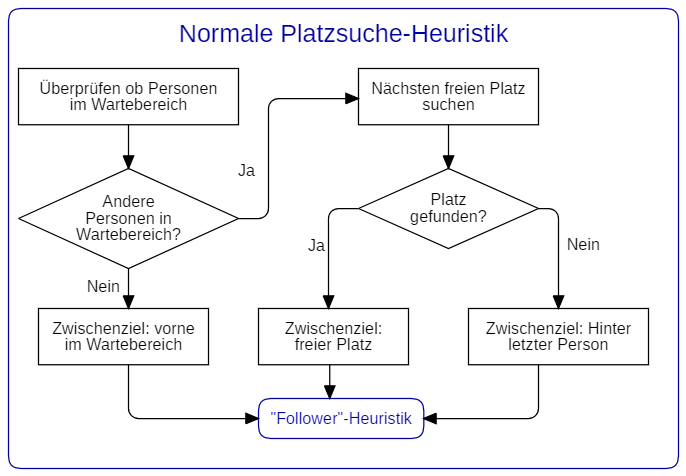
\includegraphics[width=1.0\textwidth]{pictures/model/algorithm/boarding/normal_boarding/normal_space_find_heuristic.png}
	\caption{Prozessdiagramm "`normale Platzsuche"'-Heuristik.}
	\label{fig:NPH}
\end{figure}
Will ein normaler Einsteiger sich an einen Platz im Wartebereich stellen, so wird zunächst überprüft, ob in diesem schon andere Agenten stehen. Steht dort keine Person, so wird das Zwischenziel des Agenten auf den vorderen Bereich der Wartezone gesetzt. Ich nehme an, dass jemand nah an der Tür ist, wenn er nicht weiter von ihr entfernt ist als seine doppelte Schulterbreite. Sind schon Agent im Wartebereich sucht der Agent nach dem nächsten freien Platz in der Nähe der Tür. Kann ein solcher Platz nicht gefunden werden, so wird das Zwischenziel des normalen Einsteigers zur Position hinter der letzten Person. Wurde ein freier Platz gefunden, ist dieser das Zwischenziel des Agenten. Nachdem das Zwischenziel festgelegt wurde bewegt sich der Agent mit Hilfe der "`Follower"'-Heuristik in die Richtung von diesem.
\clearpage
\begin{algorithm} [H]
	\caption{"`Normale Platzsuche"'-Heuristik}
	\SetKwInOut{Output}{Output}
	\SetKwProg{normalSpaceFindHeuristic}{normalSpaceFindHeuristic}{}{}
	
	\Output{$pos_p$ nächste gewünschte (eng.: "`preferred"') Position}
	\normalSpaceFindHeuristic{} {
		\If{andere Person in Wartebereich} {
			Suche nächsten freien Platz $pos_w$ in Wartebereich \\
			\If{Platz gefunden}{
				Ziel des auf $pos_w$ setzen \\
			}\Else{
				Ziel des Agenten auf Platz hinter letzter Person setzen  \\
			}
		} \Else {
			Ziel des Agenten auf Platz vorne im Wartebereich setzten\\
		}
		$pos_p = $ \textbf{FollowerHeuristic} \\
		\Return $pos_p$
	}
\end{algorithm}

Wie im Prozessdiagramm erklärt, wird bei der "`Platzsuche"'-Heuristik für den Einsteiger ein Zwischenziel im Wartereich gewählt. Algorithmisch wird dies Umgesetzt, indem das Ziel des Agenten auf den entsprechenden Platz gesetzt wird. Ist die Person an ihrem Zwischenziel angekommen, genügend Platz in der Tür oder alle Aussteiger ausgestiegen, so wird das Ziel des Agenten durch die vorgestellten Algorithmen für normale Einsteiger wieder auf das Innere des Zuges gesetzt. Bei den "`Platzsuche"'-Heuristiken wird in jedem Simulationsschritt erneut überprüft an welchen Platz sich die Person stellen soll. So wird verhindert, dass sich die Person auf einen Platz stellen will, an dem ein anderer Agent vor ihm ankommt.
\subsubsection{Defensiver Einsteiger}
Das Prozessdiagramm der defensiver "`Einsteiger"'-Heuristik wird in \ref{fig:DEH} gezeigt.
\begin{figure}[H]
	\centering
		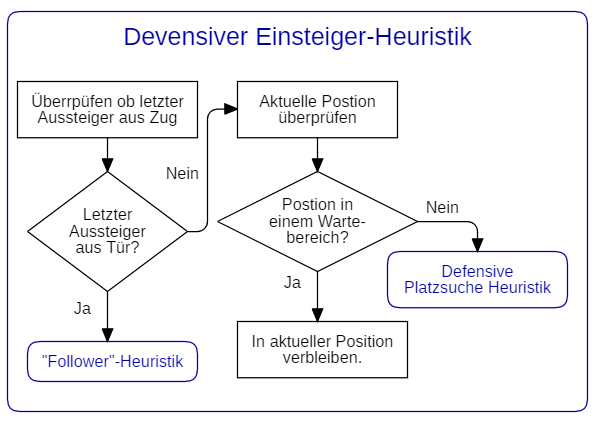
\includegraphics[width=0.9\textwidth]{pictures/model/algorithm/boarding/defensive_boarding/defensive_boarding_heuristic.png}
	\caption{Prozessdiagramm "`defensiver Einsteiger"'-Heuristik.}
	\label{fig:DEH}
\end{figure}
Wie in \figurename \ref{fig:DEH} zu sehen ist, überprüft ein defensiver Einsteiger zunächst, ob der letzte Aussteiger schon ausgestiegen ist.  Ist der letzte Aussteiger aus der Tür, beginnt der defensive Einsteiger mit der "`Follower"'-Heuristik mit dem Einsteigen. Sind noch Aussteiger im Zug, überprüft der Agent seine aktuelle Position. Liegt diese im Wartebereich, verweilte er in seiner aktuellen Position. Ist der Einsteiger noch nicht im Wartebereich, sucht er mit Hilfe der "`defensiven Platzsuche"'-Heuristik einen Platz in diesem. Diese Heuristik kann in \figurename \ref{fig:DPH} betrachtet werden. Im Gegensatz zu normalen Einsteigern, wartet der defensive Einsteiger solange im Wartebereich, bis der letzte Aussteiger den Wagon verlässt, auch wenn genügend Platz ist. 
\clearpage
\begin{algorithm} [H]
	\caption{"`Defensive Einsteiger"'-Heuristik}
	\SetKwInOut{Output}{Output}
	\SetKwProg{DefensiveBoardingHeuristic}{DefensiveBoardingHeuristic}{}{}
	
	\Output{$pos_p$ nächste gewünschte (eng.: "`preferred"') Position}
	\DefensiveBoardingHeuristic{}{
		\If{letzter Aussteiger aus Tür} {
			Ziel auf das Innere des Wagons setzen \\
			$pos_p = $ \textbf{FollowerHeuristic} \\
		} \Else {
			\If{$pos_{current}$ im Wartebereich} {
				In aktueller Position verbleiben $pos_p = pos_{current}$\\
			} \Else {
				$pos_p = $ \textbf{DefensiveSpaceFindHeuristic}	 \\	
			}
		}
		\Return $pos_p$
	}
\end{algorithm}

Bei defensiven Typen wird das Ziel erst auf das Innere des Zuges gesetzt, wenn alle Aussteiger den Zug verlassen haben. Ist dies nicht der Fall, so bleiben sie in ihrer aktuellen Position, wenn sie bereits im Wartebereich angekommen sind oder suchen mit der \textbf{DefensiveSpaceFindHeuristic} einen Platz in eben diesem.

\begin{figure}[H]
	\centering
		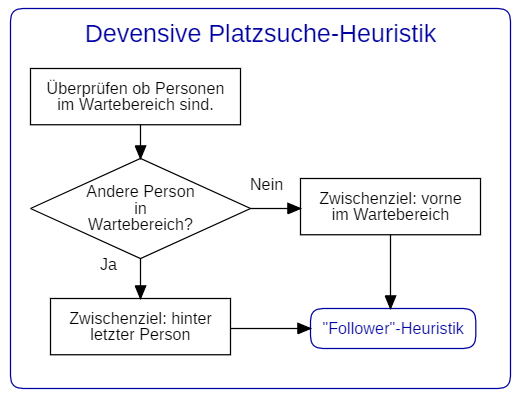
\includegraphics[width=0.8\textwidth]{pictures/model/algorithm/boarding/defensive_boarding/defensive_space_find_heuristic.png}
	\caption{Prozessdiagramm "`defensive Platzsuche"'-Heuristik.}
	\label{fig:DPH}
\end{figure}
In der "`defensiven Platzsuche"'-Heuristik, wählt der Agent als Zwischenziel ebenfalls einen Platz nahe an der Tür, wenn keine andere Person im Wartebereich steht. Ist schon eine Person im Wartebereich, so wählt der defensive Einsteiger immer die Position hinter der letzten wartenden Person im Bereich als sein Zwischenziel. Mit Hilfe der "`Follower"'-Heuristik, bewegt sich der Agent daraufhin zu seinem Zwischenziel. \\
\begin{algorithm} [H]
	\caption{"`Defensive Platzsuche"'-Heuristik}
	\SetKwInOut{Output}{Output}
	\SetKwProg{DefensiveSpaceFindHeuristic}{DefensiveSpaceFindHeuristic}{}{}
	
	\Output{$pos_p$ nächste gewünschte (eng.: "`preferred"') Position}
	\DefensiveSpaceFindHeuristic{} {
		\If{andere Person in Wartebereich} {
			Ziel des Agenten auf Platz hinter letzter Person setzen\\
		} \Else {
			Ziel des Agenten auf Platz vorne im Wartebereich setzen\\
		}
		$pos_p = $ \textbf{FollowerHeuristic} \\
		\Return $pos_p$
	}
\end{algorithm}.

Bei defensiven Agenten gibt es zwei mögliche Zwischenziele im Wartebereich. Entweder ist keine Person im Wartebereich und das Ziel der Agenten wird vom Algorithmus auf einen Platz vorne im Wartebereich gesetzt, oder der Algorithmus wählt einen Platz hinter der letzten Person im Wartebereich.
\subsubsection{Aggressiver Einsteiger}
Die Heuristik der aggressiven Einsteiger in \figurename \ref{fig:AEH} wird in \ref{fig:AEH} erklärt.
\begin{figure}[H]
	\centering
		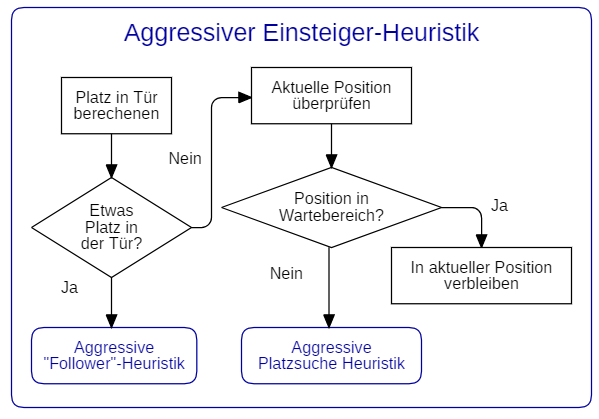
\includegraphics[width=0.8\textwidth]{pictures/model/algorithm/boarding/aggressive_boarding/aggressive_boarding_heuristic.png}
	\caption{Prozessdiagramm "`aggressive Einsteiger"'-Heuristik.}
	\label{fig:AEH}
\end{figure}
Ist etwas Platz (siehe \ref{Tabelle der Typen}) in der Tür, so beginnt der aggressive Einsteiger mit der "`aggressiven Follower"'-Heuristik mit dem Einsteigen. Er hat also eine geringere Schwelle für das Einsteigen als normale oder defensive Einsteiger, die erst bei genügend Platz oder bei Ausstieg des letzten Aussteigers mit dem Einsteigen beginnen. Ist nicht ausreichend Platz in der Tür, so wird die aktuelle Position des Agenten überprüft. Ist dieser noch nicht im Wartebereich, so sucht der aggressive Einsteiger mit der "`aggressiven Platzsuche"'-Heuristik einen Platz in diesem (siehe \figurename \ref{fig:APH}). Ist bereits im Wartebereich so verbleibt er in seiner aktuellen Position.

\begin{algorithm} [H]
	\caption{"`Aggressive Einsteiger"'-Heuristik}
	\SetKwInOut{Output}{Output}
	\SetKwProg{AggressiveBoardingHeuristic}{AggressiveBoardingHeuristic}{}{}
	
	\Output{$pos_p$ nächste gewünschte (eng.: "`preferred"') Position}
	\AggressiveBoardingHeuristic{} {
		$p=$ Platz in der Tür\\
		\If{$p \geq 0.8 \cdot $ Körperbreite} {
			Ziel auf das Innere des Wagons setzen
			$pos_p = $ \textbf{AggressiveFollowerHeuristic}
		} \Else {
			\If{aktuelle Position $pos_current$ im Wartebereich} {
				In aktueller Position verbleiben $pos_p = pos_{current}$	
			} \Else {
				$pos_p = $ \textbf{AggressiveSpaceFindHeuristic}		
			}
		}
		\Return $pos_p$
	}
\end{algorithm}

Im Algorithmus wird als Schwelle für "`etwas Platz"' in der Tür das 0.8 Fache der Körperbreite der Person verwendet. Ist dieser Platz gegeben so wird das Ziel der Person auf das Innere des Wagons gegeben. Sonst sucht der aggressive Einsteiger mit dem Algorithmus \textbf{AggressiveSpaceFindHeuristic} \ref{alg:aggressivSpaceFinder}, nach einem Platz im Wartebereich, wenn er noch nicht in diesem angekommen ist.

\begin{figure}[H]
	\centering
		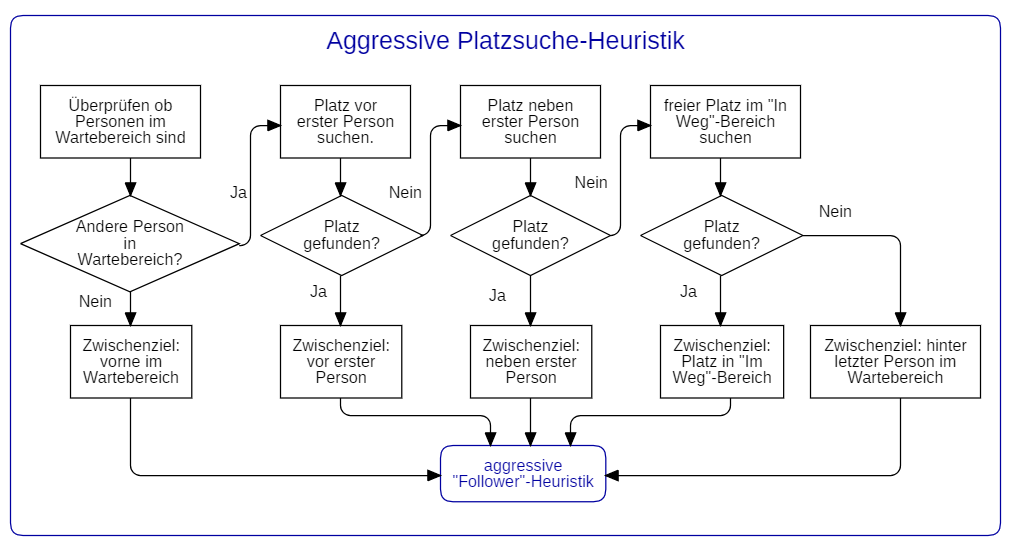
\includegraphics[width=1.0\textwidth]{pictures/model/algorithm/boarding/aggressive_boarding/aggressive_space_find_heuristic.png}
	\caption{Prozessdiagramm "`aggressive Platzsuche"'-Heuristik.}
	\label{fig:APH}
\end{figure}
Ist keine Person im Wartebereich, so wählt der aggressive Agent, genau wie ein defensiver oder normaler, einen Platz nah an der Tür als Zwischenziel. Anders als defensive und normale Typen, will der aggressive Einsteiger jedoch so weit wie möglich vorne stehen, deshalb sucht er nicht nach dem nächsten freien Platz. Stattdessen überprüft der Agent ob vor der ersten Person noch Platz ist, wobei seinem Körper auch leicht in die Tür ragen kann, wenn er sich auf diesen Platz stellt. Es ist also zu vermuten, dass für einen aggressiven Einsteiger auch Platz vor der ersten wartenden Person ist, wenn das 0.8 Fache seiner Körperbreite Platz hat. Ist hier jedoch weniger Platz, so sucht er nach einem Platz neben der ersten Person. Ist hier Platz vorhanden, so wählt er diesen als sein Zwischenziel, auch hier kann sein Körper leicht in die Tür ragen. Ist weder vor noch neben der ersten Person Platz, so sucht ein aggressiver Einsteiger nach einem Platz im "`Im Weg"'-Bereich. Dieser Bereich wurde in der Skizze der Zielbereiche für Einsteiger, \figurename \ref{fig:SkizzeEinsteiger}, bereits dargestellt. Ist hier Platz vorhanden, so wählt er wiederum diesen als Zwischenziel. Ist keiner der genannten Plätze vorhanden, so wählt der Agent als Zwischenziel den Platz hinter der letzten Person im Wartebereich. 
\clearpage
\begin{algorithm} [H]
	\caption{"`Aggressive Platzsuche"'-Heuristik}
	\label{alg:aggressivSpaceFinder}
	\SetKwInOut{Output}{Output}
	\SetKwProg{AggressiveSpaceFindHeuristic}{AggressiveSpaceFindHeuristic}{}{}
	
	\Output{$pos_p$ nächste gewünschte (eng.: "`preferred"') Position}
	\AggressiveSpaceFindHeuristic{} {
		\If{andere Person in Wartebereich} {
			Platz vor erster Person im Wartebereich $pos_{vP}$ suchen \\
			\If{Platz gefunden} {
				Ziel des Agenten auf $pos_{vP}$ setzen \\
			} \Else {
				Platz neben erster Person im Wartebereich $pos_{nP}$ suchen\\
				\If {Platz gefunden} {
				Ziel des Agenten auf $pos_{nP}$ setzen \\		
				} \Else {
					Freien Platz in "`Im Weg"'-Bereich $pos_{iW}$ suchen \\
					\If {Platz gefunden} {
						Ziel des Agenten auf $pos_{iW}$ setzen \\			
					} \Else {
						nächsten freien Platz im Wartebereich $pos_{w}$ suchen \\
						\If {Platz gefunden} {
							$Ziel = pos_w$ \\
						} \Else {
							Ziel des Agenten auf Platz hinter letzter Person im Wartebereich setzen \\					
						}
					}
				}
			} 
		} \Else {
			Ziel des Agenten auf Platz vorne im Wartebereich setzen \\
			
		}
		$pos_p = $ \textbf{AggressiveFollowerHeuristic} \\
		\Return $pos_p$
	}
\end{algorithm}

Bei aggressiven Einsteigern wird das Ziel des Agenten auf einer der möglichen Positionen gesetzt, je nachdem welche frei ist. Mit der "`aggressiven Follower"'-Heuristik bewegt sich die Person dann zu diesem Platz.

\subsection{Aussteiger-Heuristik} \label{AM}
Der Ausstiegsprozess wird mit der "`Ausstiegsprozess"'-Heuristik umgesetzt. Dabei liegt die Unterscheidung der Typen nur in der Wahl der Startzeit der Person, und der Durchführung der "`Follower"'-Heuristik.
\begin{figure}[H]
	\centering
		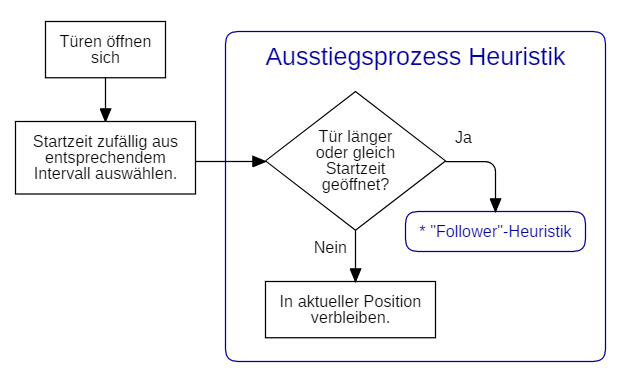
\includegraphics[width=0.8\textwidth]{pictures/model/algorithm/alight/alight_process.png}
	\caption{Prozessdiagramm der Aussteiger: "`Ausstiegsprozess"'-Heuristik.}
	\label{fig:AH}
\end{figure}
Wie in \figurename \ref{fig:AH} zu erkennen, wird die Startzeit des Aussteigers vor dem Ausstiegsprozess festgelegt. Dabei wird diese durch Zufall aus dem entsprechenden Intervall ausgewählt. Die Intervalle wurden hierbei durch die Auswertung in \ref{Startzeiten} ermittelt. Das Startzeitenintervall für defensive liegt zwischen $1.9$ und $2.1$ Sekunden. Für normale liegt es zwischen $1.6$ und $1.8$ Sekunden und für aggressive zwischen $1.3$ und $1.6$ Sekunden. Hierbei nehme ich an, dass die Werte im Intervall normal verteilt sind. Ist die Startzeit gewählt, so beginnt die "`Ausstiegsprozess"'-Heuristik. Dabei verbleibt die Person in ihrer aktuellen Position so lange nicht mehr Zeit seit der Türöffnung vergangen ist, als die Startzeit der Person. Wenn die Tür länger oder gleich der Startzeit geöffnet ist beginnt die Person mit der entsprechenden "`Follower"'-Heuristik den Ausstieg. Dabei wird die "`aggressive Follower"'-Heuristik für aggressive Typen verwendet. 
\clearpage
\begin{algorithm} [H]
	\caption{"`Ausstiegsprozess"'-Heuristik}
	\SetKwInOut{Output}{Output}
	\SetKwProg{AlightHeuristic}{AlightHeuristic}{}{}

	\Output{$pos_p$ nächste gewünschte (eng.: "`preferred"') Position}
	\AlightHeuristic{} {
		Vergangene Sekunden seit Türöffnung in $t$ speichern\\
		Typ der Person ist $T$ \\
		\If{$t <$ Startzeit des Agenten} {
			In aktueller Position verbleiben $pos_{p} = pos_{current}$ 
		} \Else {
			\If{$T$ ist aggressiv} {
				$pos_p = $ \textbf{AggressiveFollowerHeuristic}		
			} \Else {
				$pos_p = $ \textbf{FollowerHeuristic}		
			}
		}
		\Return $pos_p$
	}
\end{algorithm}

Im Algorithmus wird in jedem Schritt überprüft, ob seit der Türöffnung mehr Zeit vergangen ist ist als die Startzeit, ist das der Fall, verbleibt der Agent in seiner aktuellen Position, er wartet, bis die Türen weit genug geöffnet sind. Andernfalls steigt er mit Hilfe der Algorithmen für die "`Follower"'-Heuristik aus.

\subsection{Platzmacher-Heuristik}
Das Platzmacher-Modell wird durch die "`Platzmachprozess"'-Heuristik umgesetzt, die sowohl die "`Ausstiegsprozess"'-Heuristik, als auch die "`Einsteigeprozess"'-Heuristik verwendet.
\begin{figure}[H]
	\centering
		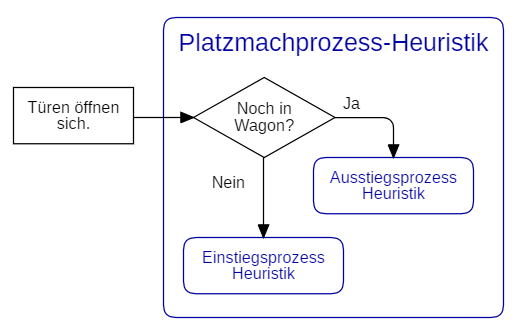
\includegraphics[width=0.7\textwidth]{pictures/model/algorithm/spacemaker/spacemaker_heuristic.png}
	\caption{Prozessdiagramm der Platzmacher: "`Platzmachprozess"'-Heuristik.}
	\label{fig:PH}
\end{figure}
Befindet sich ein Platzmacher im Wagon, so wird die "`Ausstiegsprozess"'-Heuristik (\ref{AM}) verwendet. Will eine Person aussteigen, um Platz zu machen verhält sie sich wie ein Aussteiger. Sobald die Person den Wagon verlassen hat, verhält sie sich jedoch wie ein Einsteiger, sie sucht einen Platz im Wartebereich und steigt daraufhin wieder ein. Dazu wird die "`Einsteigeprozess"'-Heuristik verwendet (\ref{EM}).

\begin{algorithm} [H]
	\caption{"`Platzmachprozess"'-Heuristik}
	\SetKwInOut{Output}{Output}
	\SetKwProg{SpacemakerHeuristic}{SpacemakerHeuristic}{}{}
	
	\Output{$pos_p$ nächste gewünschte (eng.: "`preferred"') Position}
	\SpacemakerHeuristic{} {
		\If{$pos_{current} \in $ Wagon}  {
			$pos_p = $ \textbf{AlightHeuristic}
		} \Else {
			$pos_p = $ \textbf{BoardingHeuristic}	
		}
		\Return $pos_p$
	}
\end{algorithm}

Der Algorithmus des Platzmachprozesses verwendet den Algorithmus \textbf{AlightHeuristic}, wenn sich der Agent noch im Wagon befindet. Ist der Platzmacher aus dem Wagon ausgestiegen, so wird die \textbf{BoardingHeuristic} verwendet.
\section{Modellparameter} \label{Modellparameter}
Das Fahrgastwechsel-Modell beinhaltet die Geometrie des Zuges und Bahnsteigs, sowie die jeweilige Anzahl an Einsteigern, Aussteigern und Platzmachern als Parameter. Zudem wird dem Modell auch die Geometrie der Zielbereiche und Wartereiche, sowie die Geometrie des "`Im Weg"'-Bereiches übergeben. Außerdem werden im Modell die Startzeitenintervalle, sowie der Faktor zur Überprüfung des Platzes in der Tür vorgegeben. Geometrien, für den Zug und die Bereiche, können crowd:it durch CAD Software übergeben werden. Die Parameter für die Anzahl an Einsteigern, Aussteigern und Platzmachern könnte dann in crowd:it als Zahl übergeben werden. 

Da mein Modell nicht in der Software implementiert wurde, ist nicht klar, ob Startzeitenintervalle, Faktoren für die Überprüfung nach Platz in der Tür oder andere "`Floor Field"' Parameter der Software für ein realistisches Modell noch kalibriert werden müssen. Diese Kalibrierung könnte jedoch durch die qualitative Betrachtung einer Simulation, sowie dem Vergleich des Ergebnisses der Simulation mit den ausgewerteten Daten, darunter die Wechselzeiten, stattfinden.
\chapter{Fazit und Ausblick} \label{Fazit und Ausblick}
In dieser Arbeit habe ich empirische Beobachtungen an drei großen Haltestellen der Münchner U-Bahn durchgeführt. Dabei habe ich Aufnahmen von Fahrgästen angefertigt, die ich zur Datenextraktion verwendet habe. Die von mir extrahierten Daten wurden dann in \texttt{Jupyter Notebooks} weiterverarbeitet und in Bezug auf den Fahrgastwechsel analysiert. Zum Beispiel kam ich zu dem Ergebnis, dass die Fahrgastwechselzeit der am Fahrgastwechsel beteiligten Personen aus meinen Daten durch lineare Regression abgeschätzt werden kann. Zudem wurde durch die Analyse der Daten klar, dass die Verhaltensweise "`im Weg Stehen"', wie zuvor vermutet, einen zeitlichen Einfluss besitzt. In den Daten wurde auch ein Merkmal identifiziert, dass einen signifikanten zeitlichen Einfluss besitzt. Das Merkmal "`sperrig"' trägt eine Person, wenn sie mehr Platz einnimmt als andere Personen. Eine Person ist \zB "`sperrig"', wenn sie ein großes Gepäckstück mit sich führt. Diese Art von Personen tritt an 46.43 \% der Türen auf und verlangsamt den Fahrgastwechsel, da durch sperrige Personen Fahrgäste nicht mehr zu zweit durch die Tür gehen können. Zudem ging aus meinen Daten hervor, dass es nicht nur Einsteiger und Aussteiger gibt. Es gibt es noch den sogenannten Prozesstypen Platzmacher. Dieser Prozesstyp beschreibt Fahrgäste, die nur aus dem Zug aussteigen, um Aussteigern hinter ihnen Platz zu machen. Nachdem diese Personen Platz gemacht habe steigen sie wieder in den Zug ein. Dieses Verhalten wurde an 16.07 \% der Türen gezeigt. Der Prozesstyp Platzmacher wurde als relevant eingestuft, da diese Personen sowohl aus- als auch einsteigen und somit einen signifikanten Einfluss auf die Fahrgastwechselzeit besitzen. Zudem ergab sich aus den Daten, dass es Typen von Personen gibt. Diese Typen werden auf Grund ihres Verhaltens als defensiv, aggressiv oder normal bezeichnet. Der Anteil der aggressiven und defensiven Personen ist hierbei so signifikant, dass ich ihr Verhalten im Modell umgesetzt habe. So wurde in meinem Modell zum Beispiel dargestellt, dass aggressive und normale Einsteiger "`früher einsteigen"', also einsteigen, wenn noch Aussteiger den Zug verlassen, während defensive Personen immer warten bis alle Aussteiger aus dem Zug ausgestiegen sind. Auch bei der Platzsuche unterscheiden sich die unterschiedlichen Typen. Während defensive Typen sich immer hinter die letzte Person im "`Wartebereich"' stellen, suchen normale nach dem nächsten freien Platz und aggressive stellen sich in den Weg, wenn vorne im Wartebereich kein Platz mehr ist. Ein weiteres Verhalten von defensiven Typen setzte ich ebenfalls durch kognitive Heuristik um. Defensive Typen betreten den Türbereich erst, wenn die Person vor ihr nicht mehr in diesem ist, sie warten also darauf, dass sie alleine durch die Tür gehen können. Eine weitere Unterscheidung der Typen, liegt darin, wie lange Aussteiger mit einem bestimmten Typ nach der Türöffnung warten, bevor sie mit dem Aussteigen beginnen. Dies wurde durch Intervalle für Startzeiten dargestellt, wobei Aggressive am kürzesten und Defensive am längsten warten bevor sie aussteigen.

Vergleicht man die bisherige Modellierung von accu:rate mit den gesammelten Daten, ist zu bemerken, dass dieses den absoluten Standardfall des Fahrgastwechsels ganz gut darstellen kann. In der Modellierung wird die Entscheidungsfindung der einzelnen Personen im Prozess jedoch nicht beachtet, was mein Modell verbessern soll. Ob dieses Modell jedoch wirklich zu einem besseren Ergebnis führt, wurde im Zuge dieser Bachelorarbeit jedoch nicht mehr getestet. 

Da das Modell nicht implementiert wurde, konnte ein Vergleich des Modells mit der Modellierung von accu:rate über eine Simulation nicht durchgeführt werden. Außerdem ist dadurch nicht klar, ob das Modell einen realistischen Fahrgastwechsel darstellen kann, da eine Validierung des Modells nicht durchgeführt wurde. Es wäre also interessant, dieses in eine bereits existierende Software für Fußgängersimulationen, \zB crowd:it, einzufügen, um das erstellte Modell zu Kalibrieren und Validieren, um es möglicherweise zukünftig in Planungen der MVG einsetzen zu können.

Für einige Auswertungen sind nur wenig Daten vorhanden. Durch diese geringe Datenlage, vor allem für Platzmacher und der ersten Person, die aussteigt und angibt, wie lange ein Typ vor dem Aussteigen wartet, könnte es sein, dass manche Auswertungen fehlerhaft sind. Dies könnte jedoch auch durch die Umsetzung des Modells in Software, oder durch weitere Beobachtung geprüft werden.

Wird das Modell umgesetzt und validiert, wäre es zudem noch interessant, das Modell für den Fahrgastwechsel in den Kontext eines Bahnsteiges einzufügen. Besonders interessant wäre die Kombination mit anderen Simulationsmodelle für das Innere des Zuges oder des Bahnsteigs. Diese könnten Modelle sein, die darstellen:
\begin{itemize}
\item Wie Personen einen Sitzplatz im Zug wählen (\cite{Schottl.2016} oder sich entscheiden stehen zu bleiben.
\item Wie Aussteiger sich an der Tür anstellen, um den Zug zu verlassen.
\item Wie Personen sich auf dem Bahnsteig verhalten (\cite{Davidich.2013}, \cite{Chen.2017})
\end{itemize}

Wie Einsteiger den Wagon und die Tür wählen, an der sie Einsteigen wollen, wird in meinem Modell vernachlässigt. Auch dieser Entscheidungsprozess könnte für mein Modell interessant sein, wenn nicht nur eine Tür, sondern ein gesamter Zug modelliert werden soll. Zudem erkannte ich auf den Aufnahmen auch Personen die sich zunächst an einer Tür "`anstellten"', sich dann aber doch dafür entschieden, an eine andere zu gehen. Wann dieses Verhalten auftritt könnte für die Simulationen eines Zuges interessant sein.

Das von mir erstellte Modell enthält alle als relevant erkannten Verhaltensweisen und Merkmale und könnte somit zu einem besseren Fahrgastwechsel-Modell führen, dass in der Planung von neuen Stationen oder Fahrplänen eingesetzt werden könnte. Aufgrund der geringen Datenlage und der Tatsache, dass das Modell nicht implementiert und somit nicht validiert wurde, ist es jedoch notwendig diese Implementierung nachzuholen und das Modell zu testen, bevor es eingesetzt werden kann.
\begin{appendix}
\chapter{Statistik} \label{Statistik}
\section{Lineare Regression} \label{append:LinReg}
In der linearen Regression soll der systematische Einfluss der erklärenden Variablen $x_1, \ldots, x_k$ auf die Zielvariable $y$ untersucht werden (\cite{Fahrmeir.2009}).

Bei der lineare Regression wird die Zielgröße $y$ jedoch nicht exakt als Funktion $f(x_1, \ldots x_k)$ von $x_1, \ldots, x_k$ angegeben, sondern ist eine Zufallsvariable deren Verteilung von der erklärenden Variable abhängt. "`Ein Hauptziel der Regressionsanalyse besteht somit darin, den Einfluss der erklärenden Variable auf den Mittelwert der Zielgröße zu untersuchen."' \cite{Fahrmeir.2009} Im linearen Regressionsmodellen wird unterstellt, dass die Funktion $f$, in Bezug auf $\beta_0, \ldots \beta_k$ linear, ist. Aus der Linearität ergibt sich die Funktion: 
$$ y = \beta_0 + \beta_1x_1 + \cdots + \beta_kx_k + \varepsilon_i $$
Es ist jedoch zu beachten, dass eine lineare Regression auch bei einer nicht linearen Beziehung durchgeführt werden kann. Dabei wird der nicht lineare Anteil mit den erklärenden Variablen dargestellt. So kann $x_1$ \zB durch den nicht linearen Anteil $x_1 = \log(z)$ ersetzt werden.
Die Parameter $\beta_0, \ldots, \beta_k$ werden dann basierend auf den Beobachtungen $(y_i, x_{i1}, \\ \ldots, x_{ik}) \ i=1, \ldots, n$ mit der Methode der kleinsten Quadrate so geschätzt, dass die Summe der quadrierten Abweichungen 
$$ \sum_{i=1}^{n}(y_i - \beta_0 - \beta_1x_{i1} - \cdots - \beta_kx_{ik})^2$$
der Beobachtungen $y_i$ von der Regressionsgeraden $\beta_0 + \beta_1x_{i1} + \cdots + \beta_kx_{ik}$ minimal wird (\cite{Fahrmeir.2009}).\\
Die geschätzten Parameter, die durch die Methode der kleinsten Quadrate geschätzt wurden, werden $\hat{\beta_0}, \ldots, \hat{\beta_k}$ bezeichnet. Setzt man die Schätzparameter in die Regressionsfunktion ein, so erhält man die geschätzte Regressionsfunktion:
$$\hat{y} = \hat{\beta_0} + \hat{\beta_1}x_1 + \cdots + \hat{\beta_k} + x_k$$ (\cite{Fahrmeir.2009})
\section{Logistische Regression} \label{append:LogReg}
Die logistische Regression ist eine Regression, die auf dem Logit-Modell beruht. Die Zielvariable im Logit-Modell ist binär (\cite{Fahrmeir.2009}).
Der Erwartungswert der binären Zielvariable $y$ ist dann gegeben durch:
$$\text{E}(y) = P(y=0) \cdot 0 + P(y=1) \cdot 1 = P(y=1)$$
Das Ziel der Regressionsanalyse ist also die Modellierung und Analyse der Wahrscheinlichkeit
$$P(y=1) = P(y=1 \mid x_1, \ldots, x_k) = \pi$$ 
in Abhängigkeit von den Kovariablen (\cite{Fahrmeir.2009}).
Ein lineares Modell lässt für $P(y_i=1)$ auch Werte $\pi_i < 0$ und $\pi_i > 1$ zu, was für Wahrscheinlichkeit nicht zulässig ist.
Dieses Problem kann gelöst werden, wenn man das Modell 
$$ \pi_i = P(y_i=1) = F(\beta_0 + \beta_1x_{i1} + \cdots + \beta_kx_{ik}$$
annimmt, wobei der Wertebereich der Funktion $F$ im Intervall $[0, 1]$ liegen soll. "`Wählt man die logistische Verteilungsfunktion 
$$F(\eta) = \frac{\exp(\eta)}{1+\exp(\eta)},$$
so erhält man das Logit-Modell
$$P(y_i = 1) = \frac{\exp(\eta_i)}{1+\exp(\eta_i)} $$
mit dem linearen Prädikator
$$\eta_i = \beta_0 + \beta_ix_{i1} + \cdots + \beta_kx_{ik}$$"'
\cite{Fahrmeir.2009} \\
\section{Signifikanzniveau} \label{append:Signifikanzniveau}
Das Signifikanzniveau gibt vor, welchen Wert der Wahrscheinlichkeit man als extrem unwahrscheinlich versteht. Im Fall der Hypothesentest wäre das die Wahrscheinlichkeit, dass die Werte für die Variablen unter der $H_0$ Hypothese zustande gekommen sind. Übliche Werte für $\alpha$ sind 0.01, 0.05 oder auch 0.1 (\cite{Fahrmeir.2011}).
\section{Bestimmtheitsmaß} \label{append:rsquared}
Um die Anpassung einer Regression an die Daten zu überprüfen wird das Bestimmtheitsmaß verwendet. Es wird mit $R^2$ bezeichnet und ist definiert durch
\begin{equation}
R^2 = 
\frac{\sum_{i=1}^{n}(\hat{y_i}-\bar{y})^2}{\sum_{i=1}^{n}(y_i-\bar{y})^2} = 1- \frac{\sum_{i=1}^n \hat{\varepsilon}_i^2}{\sum_{i=1}^{n}(y_i-\bar{y})^2},
\end{equation}
wobei $\hat{y_i}$ die Schätzung von $y_i$ bezeichnet. $\hat{\varepsilon}_i$ bezeichnet den Schätzfehler, also der Abweichung des Schätzwertes $\hat{y}_i$ vom wahren Wert $y_i$ der als Residuum bezeichnet wird. Der Mittelwert der beobachteten Werte wird hier mit $\bar{y}$ bezeichnet und wie folgt berechnet:
$$ \bar{y} =\frac{1}{n} \sum_{i=1}^n y_i $$ 
Für den Wert von $R^2$ gilt: $0 \leq R^2 \leq 1$ (\cite{Fahrmeir.2009}). Für das Bestimmtheitsmaß gilt: "`Je näher das Bestimmtheitsmaß bei 1 liegt, desto kleiner ist die Residuenquadratsumme und desto besser die Anpassung an die Daten."' (\cite{Fahrmeir.2009}:99).
\chapter{Ausschnitte der Tabellen}
\section{Tabelle der Fahrgastwechselzeiten}
\DTLloadrawdb{times}{../Tabellen_Notebooks/Tabels/Times.csv}
\begin{sideways}
\begin{minipage}{1.2\textwidth}
\small
\begin{tabular}{|p{1 cm} p{1.3 cm} p{1.2 cm} p{1.2 cm} p{1.2 cm} p{1.8 cm} p{1.8 cm} p{1.3 cm} p{1.8 cm} p{1 cm}|}
		\hline
		\bfseries Video & \bfseries arrival time & \bfseries station & \bfseries core alight  & \bfseries later alight & \bfseries core boarding & \bfseries later boarding & \bfseries space\-maker & \bfseries core time & \bfseries time \\
		\hline
		\DTLforeach*[\value{DTLrowi}<9]{times}%{}{}%
		{\video=Video,\aa=arrival time,\ab=station,\sp=core alight,\be=later alight,\b=core boarding,\s=later boarding,\d=spacemaker,\iw=core time,\t=time}
		{
		\\\video & \aa & \ab & \sp & \be & \b & \s &\d & \iw & \t}
	\end{tabular} \\
	\begin{tabular}{|p{1 cm} p{1.3 cm} p{1.2 cm} p{1.2 cm} p{1.2 cm} p{1.8 cm} p{1.8 cm} p{1.3 cm} p{1.8 cm} p{1 cm}|}
		\bfseries \vdots & \bfseries \vdots & \bfseries \vdots & \bfseries \vdots & \bfseries \vdots & \bfseries \vdots & \bfseries \vdots & \bfseries \vdots & \bfseries \vdots & \bfseries \vdots
		\DTLforeach*[\DTLisgt{\video}{3190}]{times}
		{\video=Video,\aa=arrival time,\ab=station,\sp=core alight,\be=later alight,\b=core boarding,\s=later boarding,\d=spacemaker,\iw=core time,\t=time}
		{
		\\\video & \aa & \ab & \sp & \be & \b & \s &\d & \iw & \t}			\\
		\hline
	\end{tabular}
	\label{tab:times}
\captionof{table}{Fahrgastwechselzeiten Tabelle: Zusatzmaterial \textsl{Times.csv}.\\ Quelle: Eigene Tabelle.}
\end{minipage}
\end{sideways}
\clearpage
\section{Tabellen der Gruppen}
\subsection{Tabelle der Gruppen für Aussteiger}
\DTLloadrawdb{aGroup}{../Tabellen_Notebooks/Tabels/Groups/GroupsAlight.csv}
\begin{table}[H]
	\centering
	\begin{tabular}{|p{1.5 cm} p{1.4 cm} p{1.4 cm} p{1.4 cm} p{1.4 cm} p{1.4 cm} p{1.4 cm} p{1.4 cm}|}
		\hline
		\bfseries Video & \bfseries 1 & \bfseries 2 & \bfseries 3  & \bfseries 4 & \bfseries 5 & \bfseries 6  & \bfseries 11 \\
		\hline
		\DTLforeach*[\value{DTLrowi}<9]{aGroup}%{}{}%
		{\video=Video,\aa=1,\ab=2,\sp=3,\be=4,\f=5,\s=6,\e=11}
		{
		\\\video & \aa & \ab & \sp & \be & \f & \s & \e}
	\end{tabular} \\
	\begin{tabular}{|p{1.5 cm} p{1.4 cm} p{1.4 cm} p{1.4 cm} p{1.4 cm} p{1.4 cm} p{1.4 cm} p{1.4 cm}|}
		\bfseries \vdots & \bfseries \vdots & \bfseries \vdots & \bfseries \vdots & \bfseries \vdots & \bfseries \vdots & \bfseries \vdots & \bfseries \vdots
		\DTLforeach*[\DTLisgt{\video}{3190}]{aGroup}
		{\video=Video,\aa=1,\ab=2,\sp=3,\be=4,\f=5,\s=6,\e=11}
		{
		\\\video & \aa & \ab & \sp & \be & \f & \s & \e}\\
		\hline
	\end{tabular}
	\caption{Anzahl der Gruppen mit bestimmter Größe für Aussteiger Tabelle: Zusatzmaterial \textsl{GroupsAlight.csv} Quelle: Eigene Tabelle.}
	\label{tab:groupsAS}
\end{table}
\subsection{Tabelle der Gruppen für Einsteiger}
\DTLloadrawdb{bGroup}{../Tabellen_Notebooks/Tabels/Groups/GroupsBoarding.csv}
\begin{table}[H]
	\centering
	\begin{tabular}{|p{1.5 cm} p{1.4 cm} p{1.4 cm} p{1.4 cm} p{1.4 cm} p{1.4 cm} p{1.4 cm} p{1.4 cm}|}
		\hline
		\bfseries Video & \bfseries 1 & \bfseries 2 & \bfseries 3  & \bfseries 4 & \bfseries 5 & \bfseries 6  & \bfseries 7 \\
		\hline
		\DTLforeach*[\value{DTLrowi}<9]{bGroup}%{}{}%
		{\video=Video,\aa=1,\ab=2,\sp=3,\be=4,\f=5,\s=6,\e=7}
		{
		\\\video & \aa & \ab & \sp & \be & \f & \s & \e}
	\end{tabular} 
	\begin{tabular}{|p{1.5 cm} p{1.4 cm} p{1.4 cm} p{1.4 cm} p{1.4 cm} p{1.4 cm} p{1.4 cm} p{1.4 cm}|}
		\bfseries \vdots & \bfseries \vdots & \bfseries \vdots & \bfseries \vdots & \bfseries \vdots & \bfseries \vdots & \bfseries \vdots & \bfseries \vdots
		\DTLforeach*[\DTLisgt{\video}{3190}]{bGroup}
		{\video=Video,\aa=1,\ab=2,\sp=3,\be=4,\f=5,\s=6,\e=7}
		{
		\\\video & \aa & \ab & \sp & \be & \f & \s & \e}\\
		\hline
	\end{tabular}
	\caption{Anzahl der Gruppen mit bestimmter Größe für Einsteiger Tabelle: Zusatzmaterial \textsl{GroupsBoarding.csv} Quelle: Eigene Tabelle. }
	\label{tab:groupsES}
\end{table}
\subsection{Tabelle der Gruppen für Platzmacher}
\DTLloadrawdb{sGroup}{../Tabellen_Notebooks/Tabels/Groups/GroupsSpacemaker.csv}
\begin{table}[H]
	\centering
	\begin{tabular}{|p{2.5 cm} p{2 cm} p{2 cm} |}
		\hline
		\bfseries Video & \bfseries 1 & \bfseries 2  \\
		\hline
		\DTLforeach*[\value{DTLrowi}<9]{sGroup}%{}{}%
		{\video=Video,\aa=1,\ab=2}
		{
		\\\video & \aa & \ab}
	\end{tabular} \\
	\begin{tabular}{|p{2.5 cm} p{2 cm} p{2 cm} |}
		\bfseries \vdots & \bfseries \vdots & \bfseries \vdots 
		\DTLforeach*[\DTLisgt{\video}{3190}]{sGroup}
		{\video=Video,\aa=1,\ab=2}
		{
		\\\video & \aa & \ab}\\
		\hline
	\end{tabular}
	\caption{Anzahl der Gruppen mit bestimmter Größe für Platzmacher Tabelle: Zusatzmaterial \textsl{GroupsSpacemaker.csv} Quelle: Eigene Tabelle.}
	\label{tab:groupsPM}
\end{table}
\section{Tabelle der Verhaltensweisen und Merkmale}
\DTLloadrawdb{Verhalten}{../Tabellen_Notebooks/Tabels/Behaviors.csv}
\begin{sideways}
\begin{minipage}{1.2\textwidth}
\small
	\begin{tabular}{|p{1 cm} p{1.2 cm} p{1.6 cm} p{1.4 cm} p{1.8 cm} p{1 cm} p{0.8 cm} p{1.8 cm} p{1.3 cm} p{1.1 cm}|}
		\hline
		\bfseries Video & \bfseries alight & \bfseries boarding & \bfseries space\-maker  & \bfseries boarding early & \bfseries bulky & \bfseries slow & \bfseries distracted  & \bfseries in way & \bfseries time \\
		\hline
		\DTLforeach*[\value{DTLrowi}<9]{Verhalten}%{}{}%
		{\video=Video,\aa=alight,\ab=boarding,\sp=spacemaker,\be=boarding early,\b=bulky,\s=slow,\d=distracted,\iw=in way,\t=time}
		{
		\\\video & \aa & \ab & \sp & \be & \b & \s &\d & \iw & \t}
	\end{tabular} \\
	\begin{tabular}{|p{1 cm} p{1.2 cm} p{1.6 cm} p{1.4 cm} p{1.8 cm} p{1 cm} p{0.8 cm} p{1.8 cm} p{1.3 cm} p{1.1 cm}|}
		\bfseries \vdots & \bfseries \vdots & \bfseries \vdots & \bfseries \vdots & \bfseries \vdots & \bfseries \vdots & \bfseries \vdots & \bfseries \vdots & \bfseries \vdots & \bfseries \vdots
		\DTLforeach*[\DTLisgt{\video}{3190}]{Verhalten}
		{\video=Video,\aa=alight,\ab=boarding,\sp=spacemaker,\be=boarding early,\b=bulky,\s=slow,\d=distracted,\iw=in way,\t=time}
		{
		\\\video & \aa & \ab & \sp & \be & \b & \s &\d & \iw & \t}\\
		\hline
	\end{tabular}
	\label{tab:Vehalten}
\captionof{table}{Verhaltenstabelle: Zusatzmaterial \textsl{Behaviors.csv}.\\ Quelle: Eigene Tabelle.}
\end{minipage}
\end{sideways}
\clearpage
\nopagebreak   
\clearpage
\section{Tabelle der Startzeiten}
\DTLloadrawdb{Startingtime}{../Tabellen_Notebooks/Tabels/TimeAfterDoorOpening.csv}
\begin{table}[H]
	\centering
	\begin{tabular}{|p{2 cm} p{2 cm} p{2 cm} p{2 cm} p{2 cm}|}
		\hline
		\bfseries Video & \bfseries Type & \bfseries Opening & \bfseries First step  & \bfseries Time \\
		\hline
		\DTLforeach*[\value{DTLrowi}<9]{Startingtime}%{}{}%
		{\video=Video,\aa=Type,\ab=Opening,\sp=First step,\be=Time}
		{
		\\\video & \aa & \ab & \sp & \be}
	\end{tabular} \\
	\begin{tabular}{|p{2 cm} p{2 cm} p{2 cm} p{2 cm} p{2 cm}|}
		\bfseries \vdots & \bfseries \vdots & \bfseries \vdots & \bfseries \vdots & \bfseries \vdots
		\DTLforeach*[\DTLisgt{\video}{3190}]{Startingtime}
		{\video=Video,\aa=Type,\ab=Opening,\sp=First step,\be=Time}
		{
		\\\video & \aa & \ab & \sp & \be}\\
		\hline
	\end{tabular}
	\caption{Startzeiten der Aussteiger für verschiedene Typen: Zusatzmaterial \textsl{TimeAfterDoorOpening.csv}. Quelle: Eigene Tabelle.}
	\label{tab:Startingtime}
\end{table}
\clearpage
\section{Tabelle der Typen}
\clearpage
\nopagebreak
\DTLloadrawdb{Types}{../Tabellen_Notebooks/Tabels/PeopleTypes.csv}
\clearpage
\begin{sideways}
\begin{minipage}{1.37\textwidth}
\small
	\begin{tabular}{|p{0.9 cm} p{1.8 cm} p{1.8 cm} p{1.8 cm} p{2.0 cm} p{1.8 cm} p{2.0 cm} p{1.5 cm} p{1.3 cm} p{1.5 cm}|}
		\hline
		\bfseries Video & \bfseries boarding defensive & \bfseries alight defensive & \bfseries space\-maker defensive  & \bfseries boarding aggressive & \bfseries alight aggressive & \bfseries space\-maker aggressive & \bfseries boarding normal  & \bfseries alight normal & \bfseries space\-maker normal \\
		\hline
		\DTLforeach*[\value{DTLrowi}<9]{Types}%{}{}%
		{\video=Video,\aa=boarding defensive,\ab=alight defensive,\sp=spacemaker defensive,\be=boarding aggressive,\b=alight aggressive,\s=spacemaker aggressive,\d=boarding normal,\iw=alight normal,\t=spacemaker normal}
		{
		\\\video & \aa & \ab & \sp & \be & \b & \s &\d & \iw & \t}
	\end{tabular} \\
	\begin{tabular}{|p{0.9 cm} p{1.8 cm} p{1.8 cm} p{1.8 cm} p{2.0 cm} p{1.8 cm} p{2.0 cm} p{1.5 cm} p{1.3 cm} p{1.5 cm}|}
		\bfseries \vdots & \bfseries \vdots & \bfseries \vdots & \bfseries \vdots & \bfseries \vdots & \bfseries \vdots & \bfseries \vdots & \bfseries \vdots & \bfseries \vdots & \bfseries \vdots
		\DTLforeach*[\DTLisgt{\video}{3195}]{Types}
		{\video=Video,\aa=boarding defensive,\ab=alight defensive,\sp=spacemaker defensive,\be=boarding aggressive,\b=alight aggressive,\s=spacemaker aggressive,\d=boarding normal,\iw=alight normal,\t=spacemaker normal}
		{
		\\\video & \aa & \ab & \sp & \be & \b & \s &\d & \iw & \t}\\
		\hline
	\end{tabular}
	\label{tab:Types}
\captionof{table}{Typen von Prozesstypen: Zusatzmaterial \textsl{PeopleTypes.csv}.\\ Quelle: Eigene Tabelle.}
\end{minipage}
\end{sideways}
\clearpage
\end{appendix}


\newpage
\thispagestyle{empty}
\mbox{}

\pagenumbering{Roman}
\setcounter{page}{0}
\bibliography{resources}
\clearpage

\thispagestyle{empty}
\mbox{}
\newpage
\thispagestyle{empty}
\begin{minipage}[b]{0.5\textwidth} 
\myname , \myvname \\
(Familienname, Vorname)
\end{minipage}
	% Auffüllen des Zwischenraums
	\hfill
	% minipage mit Grafik
\begin{minipage}[b]{0.5\textwidth}
\begin{flushright}
München, \mydate \\
(Ort, Datum)
\end{flushright}
\end{minipage}
\\\\\\\\
\begin{minipage}[b]{0.5\textwidth} 
04.11.1995 \\
(Geburtsdatum)
\end{minipage}
	% Auffüllen des Zwischenraums
	\hfill
	% minipage mit Grafik
\begin{minipage}[b]{0.5\textwidth}
\begin{flushright}
IC 8 /SS 2019 \\
(Studiengruppe / Semester)
\end{flushright}
\end{minipage}
\\ \\ \\ \\ \\
\subsection*{\centering Erklärung}
%\addcontentsline{toc}{section}{Eidesstattliche Erklärung}%\addtocontents{toc}{\vfill}
Hiermit erkläre ich, dass ich die Bachelorarbeit selbständig verfasst, noch nicht anderweitig für Prüfungszwecke vorgelegt, keine anderen als die angegebenen Quellen oder Hilfsmittel benutzt sowie wörtliche und sinngemäße Zitate als solche gekennzeichnet habe.\\\\\\\\\\
\begin{flushright}
$\overline{~~~~~~~~~~~~~~~~~~~~~~~~~~~~~~~~~~\mbox{(Unterschrift)}}$
\end{flushright}

\end{document}
